%%
%% This is file `thesis-ex.tex',
%% generated with the docstrip utility.
%%
%% The original source files were:
%%
%% uiucthesis2014.dtx  (with options: `example')
%% 
\def\fileversion{v2.25a} \def\filedate{2017/04/10}
%% Package and Class "uiucthesis2009" for use with LaTeX2e.
%\documentclass[edeposit,fullpage]{uiucthesis2009}
\documentclass[12pt, fullpage]{uiucthesis2009}

\usepackage{lineno}
%\linenumbers*[1]
\usepackage{amsmath,amssymb,amsthm,mathtools} % AMS styles for extra equation formatting
\usepackage{graphicx} % for including graphics files
\usepackage{color}
\usepackage{longtable}
\usepackage{setspace}
\usepackage{natbib}
\usepackage{nth}
\doublespacing
\fontsize{12}{15}

\setkeys{Gin}{draft=false}


\usepackage[usenames, dvipsnames]{xcolor}
\colorlet{shadecolor}{gray!5}
\usepackage{listings}
\lstset{ 
	language=bash,                     % the language of the code
	basicstyle=\scriptsize\ttfamily, 	  % the size of the fonts
	numbers=left,                   % where to put the line-numbers
	numberstyle=\tiny\color{Blue},  % the style that is used for the line-numbers
	stepnumber=1,                   % the step between two line-numbers.
	numbersep=5pt,                  % how far the line-numbers are from the code
	backgroundcolor=\color{shadecolor},  % choose the background color.
	showspaces=false,               % show spaces adding particular underscores
	showstringspaces=false,         % underline spaces within strings
	showtabs=false,                 % show tabs within strings adding particular underscores
	frame=tb,                   	  % adds a frame around the code
	rulecolor=\color{Black},        % if not set, the frame-color may be changed on line-breaks within not-black text (e.g. commens (green here))
	tabsize=1,                      % sets default tabsize to 1 spaces
	captionpos=b,                   % sets the caption-position to bottom
	breaklines=true,                % sets automatic line breaking
	breakatwhitespace=false,        % sets if automatic breaks should only happen at whitespace
	keywordstyle=\color{RoyalBlue}, % keyword style
	commentstyle=\color{OliveGreen},% comment style
	stringstyle=\color{ForestGreen} % string literal style
}



\msthesis
\title{Sensitivity of Black Carbon Aging to Modeling Assumption in CAM-chem}
\author{Yinrui Li}
\department{Atmospheric Sciences}
\schools{University of Illinois at Urbana-Champaign}
\degreeyear{2017}
\committee{Associate Professor Nicole Riemer\\
	Professor Donald Wuebbles}



\begin{document}

\maketitle

\frontmatter

%% Create an abstract that can also be used for the ProQuest abstract.
%% Note that ProQuest truncates their abstracts at 350 words.
\begin{abstract}
Black carbon (BC) aerosol strongly absorbs visible light and therefore has a warming impact on climate. Quantifying this impact requires us to develop faithful model representations of its climate-relevant properties, such as CCN activity and optical properties. One key process that needs to be captured is the BC ‘aging’ process, that is the conversion of fresh, hydrophobic black carbon into aged, hydrophilic black carbon, which directly contributes to CCN activation and wet removal and impacts black carbon’s optical properties. In current models, the BC aging timescale is either assumed to be a fixed value (1-2 days) or is determined with mechanistic transfer rates based on ad hoc aging aging criteria. Both approaches are very sensitive to the choices of assumed parameters. 

The goal of this study is to explore the sensitivity of the simulated BC burden and BC radiative forcing to the aging criterion used in CAMChem, and to compare BC aging rates in CAMChem to an aging parameterization based on more detailed particle-resolved simulations with PartMC-MOSAIC. We carried out a 1-year simulation with the global CAMChem model, where a 4-mode modal aerosol model is used. BC aerosol is transferred from a fresh, hydrophobic mode (primary carbon mode) to an aged, hydrophilic mode (accumulation mode) after condensing a certain amount of secondary materials or through coagulation. Our results show that the simulated BC burden is most sensitive to the choices of the aging criterion in the high-latitude regions, with maximum differences in the annual averaged BC mixing ratio of 16$\%$ near the surface. These differences can be higher in the monthly averaged BC mixing ratio (e.g., we observe 65$\%$ relative difference at an elevation of 10km in the Arctic for March). We also noted that SP2 instrument can capture most of BC when it is close to the source regions (internally mixed), and in the Arctic (externally mixed). The aging timescales in the CAMChem model range from less than one hour (South America) to several days (over the ocean) and these values are broadly consistent with the aging timescales from the PartMC-MOSAIC parameterization.


\end{abstract}

%% Create a dedication in italics with no heading, centered vertically
%% on the page.
\begin{dedication}
To my dearest parents for their love and support.
\end{dedication}

%% Create an Acknowledgements page, many departments require you to
%% include funding support in this.
\chapter*{Acknowledgments}

I would like to express my deepest gratitude to my advisor Prof. Nicole Riemer, who give me strong support and plentiful ideas in this project. I couldn't have accomplish this work without her encouragement and insights. I also want to thank Professor Donald Wuebbles for co-advising this project, and for providing his continuous support.

I'm thankful to the research scientists at the Los Alamos National Laboratory, Manvendra Krishna Dubey and Allison C Aiken, for collaborating on this project and sharing valuable ideas with us. Also I'm grateful to Laura Fierce, whose previous research findings shed an interesting light on our quantification of the carbonaceous aerosol aging timescales, for her enlightening guidance, and Dr. Steven Ghan at the Pacific Northwest National Laboratory, for inviting me to their Lab and helping me through the hard work of model coding.

This work was supported by the Center for Space and Earth Sciences, Los Alamos National Laboratory, Laboratory Directed Research and Development Program. So I would also like to thank them for financially supporting our project, and giving me the opportunity to work on this project.

Lastly, I would like to thank my parents for their love and accompany all the time.

%% The thesis format requires the Table of Contents to come
%% before any other major sections, all of these sections after
%% the Table of Contents must be listed therein (i.e., use \chapter,
%% not \chapter*).  Common sections to have between the Table of
%% Contents and the main text are:
%%
%% List of Tables
%% List of Figures
%% List Symbols and/or Abbreviations
%% etc.

\tableofcontents
\listoffigures

%% Create a List of Abbreviations. The left column
%% is 1 inch wide and left-justified
\chapter{List of Abbreviations}

\begin{symbollist*}
\item[BC] Black Carbon.
\item[EC] Elemental Carbon.
\item[OC] Organic Carbon.
\item[PM] Particulate Matter.
\item[VOC] Volatile Organic Components.
\item[SOA] Secondary Organic Aerosol.
\item[CCN] Cloud Condensation Nuclei.
\item[IN] Ice Nuclei.
\item[TEM] Transmission Electron Microscopy.
\item[GDE] General Dynamic Equation.
\item[MDE] Moment Dynamic Equation.
\item[MAMn] n-mode Modal Aerosol Model.
\item[SP2] Single Particle Soot Photometer.

\end{symbollist*}

%% Create a List of Symbols. The left column
%% is 0.7 inch wide and centered
%\chapter{List of Symbols}

%\begin{symbollist}[0.7in]
%\item[$\tau$] Time taken to drink one cup of coffee.
%\item[$\mu$g] Micrograms (of caffeine, generally).
%\end{symbollist}

\mainmatter
\chapter{Introduction}
	Black carbon (BC) aerosol is a product of incomplete combustion of fossil fuel, biofuel and biomass burning \citep[e.g.][]{Bond2004,forsstrom2013}. It strongly absorbs visible light and has been ranked as the second most important individual absorbing agent after CO$_{2}$, with a climate forcing of +1.1Wm$^{-2}$ \citep{Bond2013}. BC aerosols can impact the global atmospheric radiative budget by absorbing or scattering incoming solar radiation, which is called the direct effect of aerosol on climate. BC aerosols can also impact the climate by acting as cloud condensation nuclei or ice nuclei and affect cloud microphysical properties. This effect is referred to as the indirect effect of aerosols on climate. Furthermore, it can act as impurities in snow and ice after being transported to the polar regions and depositing onto their surfaces \citep[e.g.][]{zuberi2005hydrophilic,flanner2007present}. BC aerosols also have adverse impacts on air quality and human health \citep{highwood2006smoke}.
	
	Quantifying these impacts requires us to develop faithful model representations of the BC burden and its climate-relevant properties such as cloud condensation nuclei (CCN) activities and optical properties. Currently, however, significant discrepancies in model simulated BC remain in most global climate models (GCMs) and large uncertainties of its climate forcing have been shown. For example, previous studies have implied a general overestimation of BC in the mid-upper troposphere in the mid-latitudes, and an underestimation of BC in the lower and middle troposphere at high latitude \citep[e.g.][]{koch2009evaluation,schwarz2010global,fan2012easy}. The simulated BC aerosol absorption optical depth tends to be biased low compared to satellite observations \citep[e.g.][]{koch2009evaluation}. These model failures can result from the complex BC aerosol processes and properties that have not been well captured, such as its emissions, coagulation, condensation, dry deposition, and wet scavenging. \citep[][]{hakami2005adjoint,koch2009evaluation,shindell2012simultaneously}. These processes in turn control the evolution of aerosol burden, size distribution, mixing states (the level to which particles are internally or externally mixed with other species or in between), and consequently its climate forcing \citep[e.g.][]{schulz2006radiative}. 
	
	Among them, one key process that contributes to the uncertainties and thus needs to be captured is the BC ‘aging’ process, the conversion of freshly emitted, hydrophobic BC to aged, hydrophilic BC through coating with sulfate and organics or coagulation \citep[][]{langner1992periodicity,parungo1994aeolian,liousse1996global}. This process directly contributes to the CCN activation and wet removal, and also impacts black carbon's optical properties by evolving the composition and mixing states of aerosols. Therefore, it plays a significant role in simulating the lifetime of BC, and hence its transport, distributions and climate effects \citep[e.g.][]{croft2005black,riemer2004soot}. In addition, previous studies have found that the parameterizations of the aging process can significantly affect model results \citep{Liu2010}.
	
	Albeit its importance, the treatment of BC aging, however, is usually very simplified in global scale models by using fixed timescales or parameterized aging rates for the sake of computational limits. The most simplified bulk schemes assume fully externally mixed populations and often use a fixed aging timescale (on the order of 1-2 days) for conversion of hydrophobic BC to hydrophilic BC (Cooke and Wilson, 1996). There are also more advanced schemes such as the modal aerosol model or sectional models, computing mechanistic transfer rates by assuming aerosol size distributions and mixing levels \citep[e.g.][]{bauer2013historical,huang2013enrichment}. 
	
	The representation of BC aging in the Community Atmosphere Model with Chemistry (CAM-Chem), an atmospheric component of the Community Earth System Model (CESM), uses the latter scheme. It applies a four-mode version of the Modal Aerosol Model (MAM4), where BC is emitted to the primary carbon mode, and then is aged and transferred to the accumulation mode by condensation of sulfate, ammonia and SOA and by coagulation \citep[e.g.][]{Liu2012,Lamarque2012}. In MAM4, a criterion of eight-monolayers of sulfate is used to compute the aerosol transfer rate from primary carbon mode to accumulation mode. It assumes that BC particle is aged after condensing an equivalent of eight-monolayers of sulfate. However, previous studies have shown that considerable sensitivities exist regarding the choices of the number of monolayers and other parameters, and significant model biases in BC burden have been found compared to HIPPO observations \citep{Liu2010}. 
	
	Furthermore, \citet{Fierce2016} has derived a parameterization that characterizes the aging rates of BC aerosols through gas condensation and particle coagulation from detailed simulations on the particle scale, based on the particle-resolved PartMC-MOSAIC model (Particle Monte Carlo Model for Simulating Aerosol Interactions and Chemistry) \citep{Fierce2016}. PartMC-MOSAIC is a complex aerosol model that provides detailed information on aging processes at the micro-scale, by tracing the size, composition and mixing states of particles \citep{riemer2010introducing}. The aging parameterization put forward by \citet{Fierce2016} can be used to evaluate and to improve the treatment of BC aging in the global-scale models. 
	
	In this work, our aim is to assess the representation of BC aging in MAM4 of the CAMChem model. We conducted several sensitivity runs by varying the BC aging criterion, in order to investigate the extent to which the BC mixing ratio, mixing states and direct radiative forcing are sensitive to the choices of aging parameters. We also exploit the PartMC-MOSAIC parameterization as the reference to evaluate the performance of MAM4 aging scheme. 
	
	\chapter{Background and Motivation}
	In this chapter, starting with an introduction to atmospheric aerosols, and more specifically the BC-containing aerosols, we give a broad view of their size distribution, chemical compositions and mixing state, in preparation for the further discussion of their measurements and representation in numerical models. We then explain the mixing state impact on climate and the benefits and limits of SP2 measurements. Model simulation of aerosols is discussed at the end of this chapter, including the general aerosol dynamic modeling, CAM-chem modal aerosol modeling (MAM) and Particle Resolved Aerosol Modeling.
	
	\section{Atmospheric Aerosol and its Particle Size Distribution}
	An atmospheric aerosol is a multiphase system containing gases with suspended particles in the air. They can come from either natural sources or anthropogenic sources, such as dust and sea salt that arises without human intervention, pollen and plant debris that originate from biological processes, and vehicle and industrial combustions that come from human activities. Figure~\ref{fig_P25} illustrates the aerosol life cycle in the atmosphere, including their sources, physical and chemical processes during their formation and transport, and their deposition. 
	
	As a result, aerosols can change the composition of the atmosphere and cause important environmental and climate effects. For example, carbonaceous aerosol has been associated with natural and anthropogenic air pollution, reduced visibility, climate change, and adverse health effects \citep{Mauderly2008}. One of the most important parameters that affect the transport scale and the environmental and climate properties of atmospheric aerosols is the size of their particles \citep{Pacyna1995}. Figure~\ref{fig_P26} shows the size distributions of the equivalent aerodynamic diameter of aerosols (the diameter of a spherical particle with the same value of some physical property as the irregular particle), and their categorization into modes with respect to their sizes and origins. Generally, the nucleation mode consists of particles smaller than $10^{-2}\mu$m, formed by nucleation of supersaturated vapors. They grow in size by condensation of vapor and coagulation with other particles, and can form Aitken mode ($10^{-2}$~$\mu$m~--$10^{-1}$~$\mu$m) and accumulation mode ($10^{-1}$~$\mu$m~--1~$\mu$m). Particles above the diameter size of 1~$\mu$m form the coarse mode. They are produced by mechanical processes such as the fragmentation of solids and atomization of liquids \citep{Pacyna1995,kulmala2004}.
	The nucleation mode and Aiken mode account for most of the number of the aerosol population, whereas the accumulation and coarse mode account for most of the mass. 
	
	\begin{figure}[h] 
		\begin{center}
			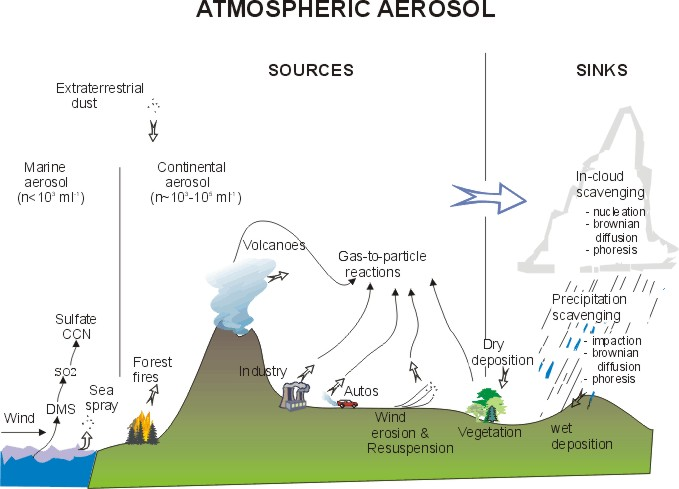
\includegraphics[width = 0.6\textwidth]{Figure25}
			\caption[Overall life cycle of atmospheric aerosols]{\label{fig_P25} Overall life cycle of atmospheric aerosols. (http://www.ems.psu.edu/lno/Meteo437/Aerosol.jpg)}
		\end{center}
	\end{figure}
	
		\begin{figure}[h] 
			\begin{center}
				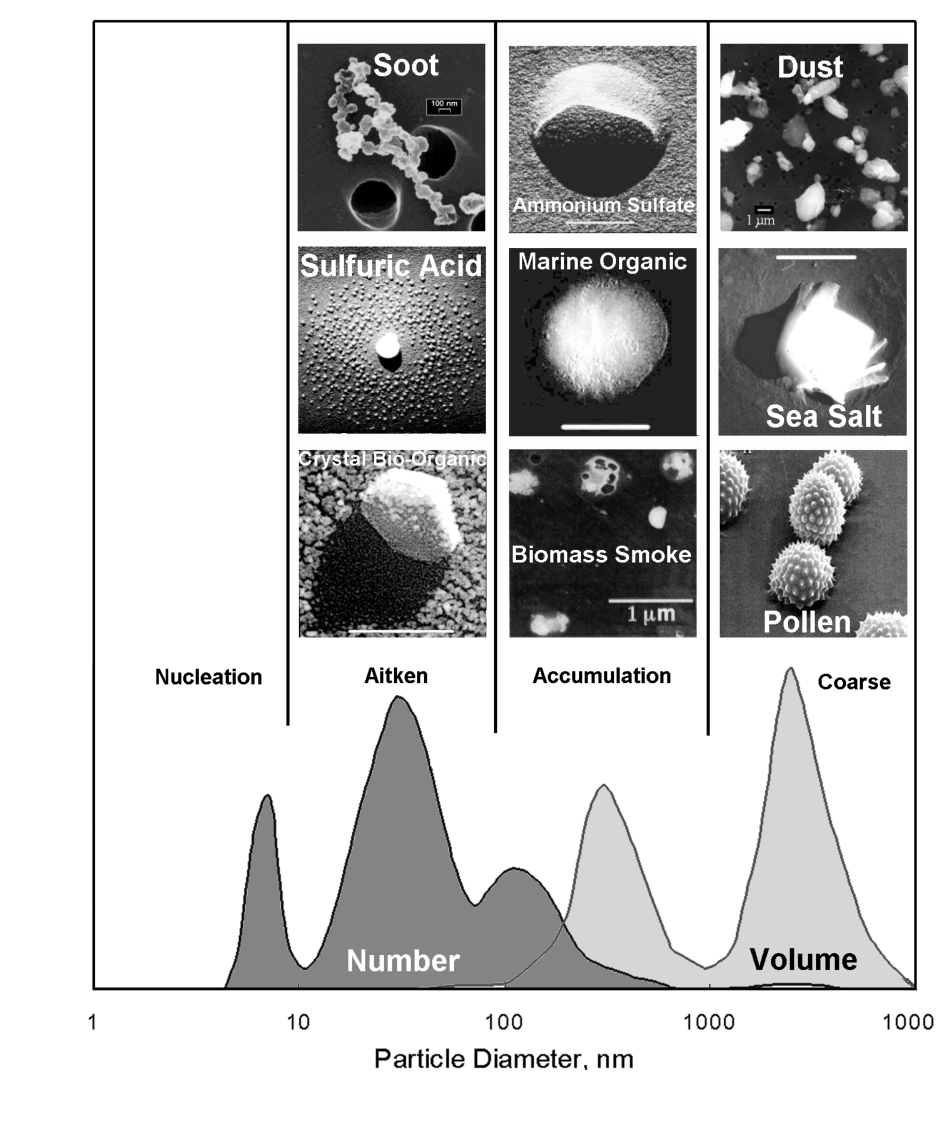
\includegraphics[width = 0.6\textwidth]{Figure26}
				\caption[Atmospheric aerosols and their size distributions]{\label{fig_P26} Atmospheric aerosols and their size distributions. \\ (http://capita.wustl.edu)}
			\end{center}
		\end{figure}

	\section{Composition of Atmospheric Aerosol and its Mixing State}
	\subsection{Chemical Composition of Atmospheric Aerosol}
	Atmospheric aerosols can be formed either by direct emissions from sources such as incomplete combustion and wind-driven suspension of solids (primary particle), or by gas--to--particle conversion (secondary particle). Sulfate, nitrate, ammonium, chloride, sea salt, mineral dust, organic components and black or elemental carbon are the predominent components of the air particulate matters (PM) \citep{poschl2005}. Figure~\ref{fig_P27} shows the average mass concentration and chemical composition of the non-refractory submicron particles based on the AMS datasets.
	
	Organic species represent one major fraction (20--90~$\%$) of the aerosol mass. The primary organic aerosols are emitted directly as liquid or solid particles or as semivolatile vapors, and the secondary organic aerosols are formed by gas--to--particle conversion of volatile organic components (VOCs). The main sources of organic species include natural or anthropogenic biomass burning, fossil-fuel combustion and biological materials (plants, pollen, animal debris)\citep{poschl2005}. Another main components of air aerosol mass are carbonaceous species that consist of black carbon (BC) or elemental carbon (EC) and organic carbon (OC). Freshly emitted BC particles are mostly hydrophobic, and the particles tend to grow hygroscopic via condensation of secondary organic and inorganic species and coagulation with soluble aerosols \citep{riemer2010estimating}. The composition of carbonaceous aerosols is dependent on the fuel type and combustion activities.
	
	Figure~\ref{fig_P5} shows an observation of the chemical species compositions of single aerosol particles, measured by transmission electron microscopy (TEM). It is obvious that most aerosols are not pure, and can be mixed with other species. In addition, the composition can be highly variable spatially. 
	\begin{figure}[h] 
		\begin{center}
			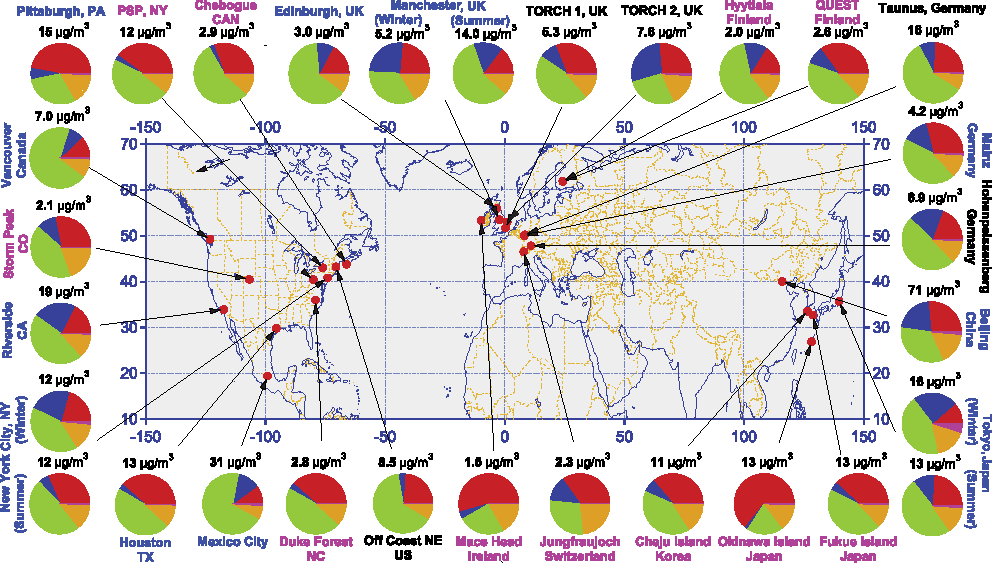
\includegraphics[width = 0.8\textwidth]{Figure27}
			\caption[Location of the AMS datasets analyzed in \citet{Zhang2015}. Pie charts show the average mass concentration and chemical composition: organics (green), sulfate (red), nitrate (blue), ammonium (orange), and chloride (purple)]{\label{fig_P27} Location of the AMS datasets analyzed in \citet{Zhang2015}. Pie charts show the average mass concentration and chemical composition: organics (green), sulfate (red), nitrate (blue), ammonium (orange), and chloride (purple).}
		\end{center}
	\end{figure}
	
		\begin{figure}[h] 
			\begin{center}
				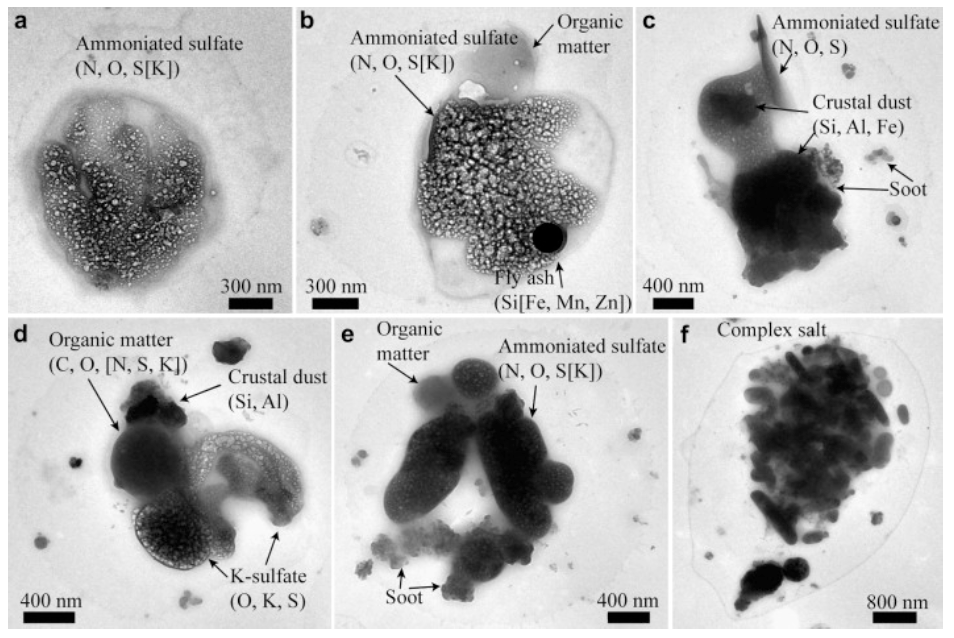
\includegraphics[width = 0.8\textwidth]{Figure05}
				\caption[Chemical species mixing and compositions of aerosol particles, taken from the . (Li et al., 2011b)]{\label{fig_P5} Chemical species mixing and compositions of aerosol particles (Li et al., 2011b).}
			\end{center}
		\end{figure}
	
	
	\subsection{Aerosol Mixing States}
	We have mentioned in the previous section that most aerosols are not pure, and can be mixed with other species. The degree to which particles are internally or externally mixed with other species or in between are called 'mixing state'.  

	\subsubsection{A Quantitative Metric}
	\citet{Riemer2013} has developed the first quantitative metric to represent the mixing state of aerosol population using a mixing ratio index $\chi$ defined as the ratio of per particle diversity $D_{\alpha}$ to the bulk population diversity $D_{\gamma}$. It ranges from $\chi = 0$ when all particles are fully externally mixed to $\chi = 1$ when all particles are fully internally mixed. Figure~\ref{fig_P28} illustrates the relationship between per--particle diversity $D_{\alpha}$, bulk diversity $D_{\beta}$, and mixing state index $\chi$.
	
	The initial mixing state can be further modified in the atmosphere as particles evolve. Taking carbonaceous aerosols for example, freshly emitted BC aerosols are mostly hydrophobic and externally mixed. During their transport, they tend to become more hydrophilic and internally mixed as a result of the aging process~--the condensation of secondary organic and inorganic species and coagulation with soluble aerosols. Figure~\ref{fig_P6} shows the evolution of the carbonaceous aerosol mixing states with time. As a result, the accuracy of BC mixing state and related climate properties greatly depend on the representation of the aging process in models.
	
	 \begin{figure}[h] 
	 	\begin{center}
	 		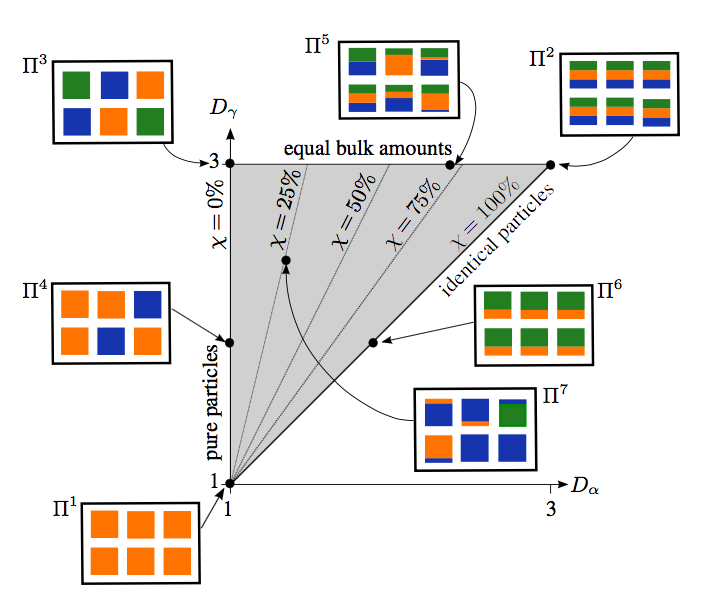
\includegraphics[width = 0.8\textwidth]{Figure28}
	 		\caption[Mixing states diagram to illustrate the relationship between per--particle diversity $D_{\alpha}$, bulk diversity $D_{\beta}$, and mixing state index $\chi$ \citep{Riemer2013}]{\label{fig_P28} Mixing states diagram to illustrate the relationship between per--particle diversity $D_{\alpha}$, bulk diversity $D_{\beta}$, and mixing state index $\chi$ \citep{Riemer2013}.}
	 	\end{center}
	 \end{figure}
	
	\begin{figure}[h] 
		\begin{center}
			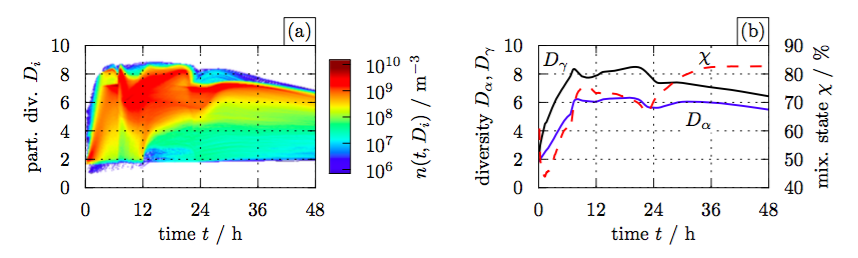
\includegraphics[width = 1\textwidth]{Figure06}
			\caption[Diversity and mixing state evolution for BC-containing particles in the urban plume case. (a) Distribution of per-particle diversity $D_{i}$ as a function of time. (b) Time series of average per-particle diversity $D_{\alpha}$, bulk diversity D$D_{\gamma}$, and mixing state index $\chi$ \citep{Riemer2013}]{\label{fig_P6} Diversity and mixing state evolution for BC-containing particles in the urban plume case. (a) Distribution of per-particle diversity $D_{i}$ as a function of time. (b) Time series of average per-particle diversity $D_{\alpha}$, bulk diversity $D_{\gamma}$, and mixing state index $\chi$ \citep{Riemer2013}}
		\end{center}
	\end{figure}
	
	\subsubsection{Mixing State Impact on Climate}
	Current representation of aerosol and its impact on climate in global models still has large uncertainties, mostly due to the difficulties to capture the microphysical and chemical processes that drive the evolution of aerosol particles in the atmosphere. Several studies have implied that the mixing states affect the climate-related aerosol properties such as optical properties or cloud condensation nuclei activity \citep[e.g.][]{jacobson2001strong,zaveri2010contributions,koch2009evaluation}. In addition, \citet{Reddington2013} has found that the model-observation biases in BC properties are much greater than for the overall particle distribution, indicating that the model discrepancies can be largely due to the assumptions about the size and mixing state of the emitted carbonaceous particles. 
	
	Efforts to improve the representation of aerosol mixing states in both regional and global models have also been made  \citep[e.g.][]{jacobson2001strong,Riemer2013}. \citet{Riemer2013} has pointed out that the mixing state of carbonaceous particles depends strongly on the fuel and combustion type. In our study, we computed the average population hygroscopicity $\kappa$ as an implication to mixing states for each mode of the four-mode modal aerosol model (MAM4) in CAM-chem.
	
	\subsubsection{BC-containing Aerosols}
	BC-containing aerosols can affect climate in multiple ways. They have both direct and indirect effects as atmospheric aerosols, and can reduce the surface albedo after depositing onto snow or ice. The BC component of its aerosols strongly absorbs solar radiation at visible wavelength, however, it can also be mixed with hydrophilic materials such as nitrate, sulfate or secondary organic aerosols (SOA) and act as CCN or IN. The mixing state of atmospheric BC particles with those hydrophilic aerosol components can affect both their CCN/IN activities and radiative properties \citep[e.g.][]{cheng2006}. Previous study has found that the light absorption of BC particles can be enhanced by 50 to 60~$\%$ after adding non-BC materials, and the enhancement is determined by the particles' mass ratio of non--black carbon \citep{liu2017black}. 
	
	In addition, current atmospheric models used to quantify the climate effects of black carbon aerosols are to be improved due to the uncertainties in simulating the complex processes such as BC aerosol formation, aging, cloud interaction, and deposition \citep{Kipling2016}. This implies that the model predicted BC aerosol mixing state are generally not in agreement with the observations \citep{Raatikainen2015}. 
	
	\section{Measurements of Carbonaceous Aerosols}
	State measurements are required in order to assess the accuracies of model simulated BC aerosol concentrations, mixing states and climate effect, and to improve model parameterizations \citep[e.g.][]{Reddington2013}. However, although many measurements of BC aerosols have been launched, few instruments are able to measure their mixing state. In recent years, one advanced observation technique using laser-induced incandescence, called the Single Particle Soot Photometer (SP2), has been developed to measure the mass distribution and mixing state of refractory black carbon (rBC) \citep[][]{baumgardner2004warming,schulz2006radiative}. It is one of the most widely used instruments for BC aerosols. 
	
	The single particle soot photometer (SP2) quantifies refractory black carbon (rBC) mass by using a laser to heat rBC to incandescence and measuring its emitted thermal radiation (Figure~\ref{fig_P9}). It measures the masses of BC particle cores over a calibrated volume equivalent diameter (VED) range of 55--400~nm. This method is suited for the detection of BC mass in the accumulation mode \citep{schwarz2010global}, but unlikely to represent the total ambient number and mass concentrations of BC particles. The SP2 number-detection efficiency at sea level pressure is reported to be 100$\%$ for BC above 90~nm VED \citep{schwarz2010global} (Figure~\ref{fig_P8}), so following \citet{Reddington2013}, we regarded 90~nm--400~nm as the diameter range that can be detected by SP2 instruments with $>$90~$\%$ efficiency and so that can be relevant when comparing model results to SP2 measurements.
	
	In order to compare model simulated BC to observations, it is important to first make sure that most of the modeled BC mass is in the size range of SP2 measurements (e.g., in source regions, freshly emitted BC can be smaller than 100~nm). In our study, we estimated the mass fraction of modeled BC in the size range corresponding to SP2 measurement in preparation for further comparison with observations, especially in the Arctic region.
	
	\begin{figure}[h] 
		\begin{center}
			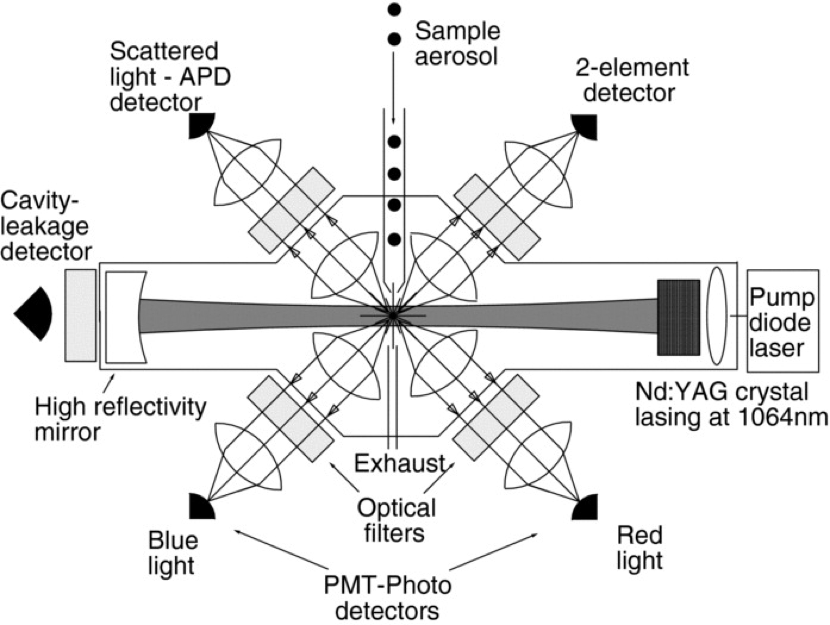
\includegraphics[width = 0.7\textwidth]{Figure09}
			\caption[Schematic of the Single Particle Soot Photometer (SP2) \citep{schwarz2010global}.]{\label{fig_P9} Schematic of the Single Particle Soot Photometer (SP2) \citep{schwarz2010global}.}
		\end{center}
	\end{figure}
	
	\begin{figure}[h] 
		\begin{center}
			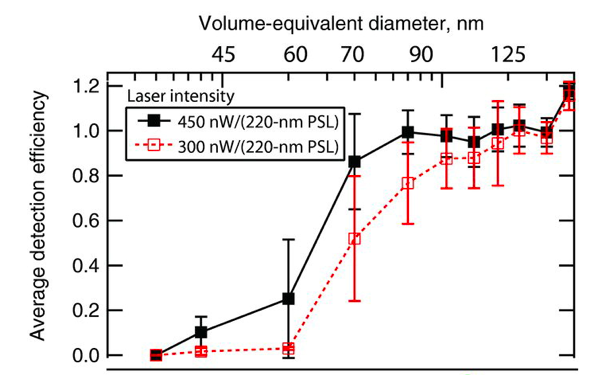
\includegraphics[width = 0.7\textwidth]{Figure08}
			\caption[The average detection efficiencies in each rBC mass-bin for each laser intensity shown in the legend. Whiskers represent the standard deviation of the values in each mass bin. The top axis shows volume-equivalent diameter (assuming 2 g/cc void-free density for rBC) that corresponds to denuded rBC-core mass on the bottom horizontal scale \citep{schwarz2010global}]{\label{fig_P8} The average detection efficiencies in each rBC mass-bin for each laser intensity shown in the legend. Whiskers represent the standard deviation of the values in each mass bin. The top axis shows volume-equivalent diameter (assuming 2 g/cc void-free density for rBC) that corresponds to denuded rBC-core mass on the bottom horizontal scale \citep{schwarz2010global}.}
		\end{center}
	\end{figure}

\newpage

	\section{Model Simulations on Aerosol Evolution}
		\subsection{Aerosol Dynamic Modeling}
		During their lifetime in the atmosphere, aerosols undergo complex physical and chemical processes. A numerical aerosol model can serve as useful tool to gain process-level understanding of the aerosol evolution in the atmosphere. Generally, an aerosol model should be able to represent the relevant processes including coagulation, condensation of secondary inorganic and organic species, nucleation, emission and chemical reaction. \citep{whitby1997}. The approaches to solve those expressions differ by the way that aerosols are approximated. Some traditional models represent aerosols as a bulk population or as a function of single variable such as their mass. More computationally demanding models include sectional models that sets discrete size bins and typically assumes species to be internally mixed with the pre--existing aerosols in each bins and externally mixed between different bins \citep[][]{jacobson2001strong,adams1999global}. This approach neglects the aging process by assuming particles to be internally mixed immediately after emission. Another frequently--used representation is called the modal aerosol model \citep[][]{whitby1997,Binkowski1995}. Aerosols are viewed as distinct populations of particles that is distinguished by their size or chemical composition, and the size distribution of each population is approximated by some analytical distribution function \citep{Binkowski1995}. Each region of the size distribution is called a mode. The size of the particles in each population is typically approximated by a lognormal distribution characterized by the mean diameter $\mu$ and a standard deviation $\sigma$. The accuracy of the model largely depends on how well the size distribution functions of the modes can represent the actual aerosol size distributions.  
		
		\begin{figure}[h] 
			\begin{center}
				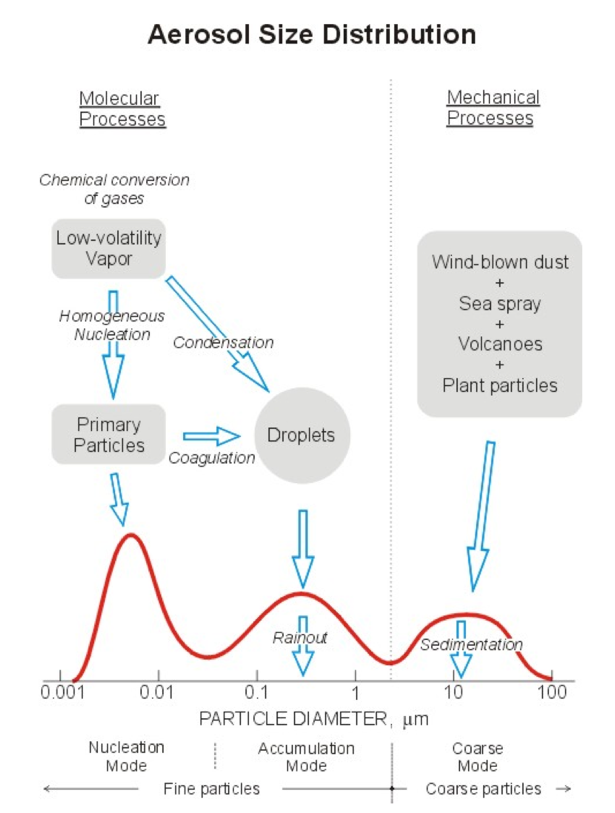
\includegraphics[width = 0.6\textwidth]{Figure04}
				\caption[Aerosol Size Distribution. (www.ems.psu.edu/\~lno/Meteo437]{\label{fig_P4} Aerosol Size Distribution. (www.ems.psu.edu/\~lno/Meteo437)}
			\end{center}
		\end{figure}
		\subsubsection{Moment and Moment Dynamic Equation}
		Modal aerosol models typically assume lognormal size distributions for each mode (Equation~\ref{eq:1}) by setting a mean diameter $D_{\rm g}$ and a standard deviation $\sigma_{\rm g}$. 
		\begin{align}\label{eq:1}
		n(\text{ln}D) = \frac{N}{\sqrt{\pi}\text{ln}\sigma_{\rm g}}\text{exp}[-\frac{1}{2}(\frac{\text{ln}(D/D_{\rm g})}{\text{ln}\sigma_{\rm g}})^2]
		\end{align}
		We can predict how the size distribution evolves if we know how the three parameters, $D_{\rm g}$, $N$, and $\sigma_{\rm g}$ evolve in the response to the microphysical and chemical processes such as nucleation, coagulation and condensation. During each time step, the model will update the geometric mean diameter $D_{\rm g}$, total number concentration $N$ and standard deviation $\sigma_{\rm g}$ for each mode, solved from their aerosol dynamic differential equations. 
		
		However, while the differential equations for the total number $N$ is easy to obtain, it is hard to find the analogous equations for $D_{\rm g}$ and $\sigma_{\rm g}$. In order to avoid this problem, an integral form, called moment, is hence introduced to replace the traditional form of differential equations. The mathematical expression of the kth moment is defined as:
		\begin{align}
		M_\text{k} = \int_{-\infty}^{+\infty}D^kn(\text{ln}D)d\text{ln}D = ND_{\rm g}^k\text{exp}[\frac{k^2}{2}\text{ln}^2\sigma_{\rm g}],
		\end{align}
		\begin{flushleft}
			$k = 0$ : total number $N = M_0$, \\
			$k = 2$ : total surface area $S = \pi M_2$, \\
			$k = 3$ : total volume $V = \frac{\pi}{6}M_3$, \\
		\end{flushleft}
		where the total number, surface area and volume of particles in one mode are proportional to the \nth{1} moment, \nth{2} moment and \nth{3} moment respectively. 
		
		The general dynamic equation (GDE) for aerosols can be found in \citet{whitby1997} (equation 4). Here we only show an analogous form of the general dynamic equation written for the change of moments, $M_{k}$, called the moment dynamic equation (MDE):
		
		\begin{align}\label{eq:2}
		\begin{split}
		\frac{\partial M_\text{k}(t)}{\partial t} = &
		\underbrace{\nabla \cdot vM_k}_\text{\clap{advection}} - \underbrace{\nabla \cdot \int_{0}^{\infty}D^k\times c(D,t)n(D,t)dD}_\text{\clap{external forces}} \\
		&+ \underbrace{\nabla \cdot \int_{0}^{\infty}D^k\times D(D,t)\nabla n(D,t)dD}_\text{\clap{diffusion}} \\
		&+ \underbrace{\int_{0}^{\infty}\frac{dD^k}{dV(D)}\times \frac{\partial V(D)}{\partial t}\times n(D,t)dD}_\text{\clap{condensation/evaporation}} \\
		&+ \underbrace{\int_{0}^{\infty}D^k\times \dot n(D,t)dD}_\text{\clap{nucleation}} \\
		&+ \underbrace{\frac{1}{2}\int_{0}^{\infty}\int_{0}^{\infty}
			(D_{1}^3+D_{2}^3)^{\frac{k}{3}}\times \beta(D_{1},D_2)\times n(D_1, t)\times n(D_2,t) dD_1dD_2}_\text{\clap{coagulation gain}} \\
		&-\underbrace{\frac{1}{2}\int_{0}^{\infty}\int_{0}^{\infty}
			(D_{1}^k+D_{2}^k)\times \beta(D_{1},D_2)\times n(D_1, t)\times n(D_2,t) dD_1dD_2}_\text{\clap{coagulation loss}}
		\end{split}
		\end{align}
		In Equation~\ref{eq:2}, $c(D,t)$ is the setting velocity, $D(D,t)$ is the diffusion rate, $n(D,t)$ is the particle number distribution, $\beta(D_{1},D_2)$ is the coagulation coefficient of particles with geometric size of $D_1$ and $D_2$, and $V(D)$ is the volume distribution of particles. The coagulation terms only represent intramodal coagulation here. When there are more than 2 modes, the equation will include more coagulation terms in the same form as the fifth and sixth term, in order to represent intermodal gain and loss due to coagulation.
		
		Generally, modal aerosol models will solve the moment differential equations for $M_0$, $M_3$ and $M_6$, and then derive $N$, $D_{\rm g}$ and $\sigma_{\rm g}$ from the three moments. $M_6$ is chosen because the coagulation term can be integrated analytically.
		 
		\subsection{Modal Aerosol Model (MAM) in CAM-chem}
		Figure~\ref{fig_P4} shows a typical categorization of aerosols by their size distributions. Particles less than 0.1~$\mu$m form the nucleation mode, particles in the size range 0.1--2~$\mu$m form the accumulation mode, and particles larger than 2~$\mu$m form the coarse mode. Similarly, in the CAM-chem model, a three-mode version of modal aerosol model (MAM3) that has only Aitken, accumulation and coarse mode was developed as default, which is efficient for long-term simulations \citep{Liu2012}. The four-mode version (MAM4) has an additional primary carbon mode added to MAM3 for the treatment of the microphysical aging processes of primary carbonaceous aerosols \citep{Liu2016}, and a seven mode version (MAM7) that has Aitken, accumulation, primary carbon, fine dust and fine sea salt, coarse dust and coarse sea salt modes \citep{Liu2012}. MAM7 has similar treatment of the aging process as in MAM4, but it also separates out sea salt and dust.
		
		We used MAM4 in our study. More description about MAM4 is in Section 3.1. MAM4 assumes that the standard deviation $\sigma_{\rm g}$ for each mode is fixed, whereas $N$ and $D_{\rm g}$ evolve with time. For each time step the model will solve the dynamic differential equations for $M_0$ and $M_3$, and then derive $N$ and $D_{\rm g}$ from the two moment equations.
		
		\subsection{Particle Resolved Aerosol Modeling}
		To complement our study of carbonaceous aerosol aging timescales, we need a more complex and precise model as a reference to the global model simulated results. 
		
		The particle resolved Monte Carlo (PartMC) model offers a way to explicitly resolve and tracks the composition of individual aerosol particles in a well-mixed volume \citep{riemer2009simulating}. Coagulation, advection and diffusion are simulated stochastically. It is also coupled with the model for simulating aerosol interactions and chemistry (MOSAIC) to simulate the gas-phase chemistry and dynamic gas particle mass transfer \citep{zaveri2008model}. 
		
		The PartMC-MOSAIC model predict the evolution of mass and composition of individual particles, and hence their mixing states and climate related properties (e.g., CCN property, optical depth property) without making simplified assumptions. So the errors of simulated aerosols and their aging processes can be reduced. In this sense, it has the benefit over the traditional sectional or modal models that often make assumptions for aerosol distribution, mixing states and the condensation and coagulation processes.
		
	\chapter{Methodology}
	In this chapter, we will discuss the CAM-chem model configuration, the condensation criterion for BC aging and its mathematical representation. Also, we will explain the first-order BC aging timescale extracted from CAM-chem model, and the PartMC-MOSAIC parameterization of aging that can be used an a reference for global models.
	
	\section{CAM-chem Model Configurations and MAM4}
	
	The CAM-chem model is a global 3-D atmospheric component of the NCAR Community Earth System Model (CESM). It consists of the Community Atmosphere Model (CAM) model and chemical mechanism of a fully implemented model for ozone and related chemical tracers (MOZART-4) which includes 191 chemical tracers and over 400 reactions. The CAM-chem model can be run either with interactive meteorology coupled to a free-running ocean with specified sea ice and sea surface temperature (free-running configuration), or with specified meteorology which read in winds, air temperature, surface pressure and heat fluxes (offline configuration) \citep{Lamarque2012}. It is also coupled to the land model, involving emissions from biogenic sources by the Model of Emissions and Aerosols from Nature (MEGAN). 
	
	For our study, we chose the CESM 1-2-2 CAM-chem configured with the offline meteorological data from the Global Earth Observing System (GEOS-5) of the Global Modeling Assimilation Office of NASA, and launched one-year simulation for 2010 with a standard horizontal resolution of 1.9  latitude by 2.5 longitude and a vertical resolution of 56 layers in order to match the resolution of the input meteorology field. We use the Intergovernmental Panel on Climate Change (IPCC) Fifth Assessment report (AR5) gridded POM and BC emissions for the period 1850-2010 in decadal increments \citep{Lamarque2010}. This inventory covers a wide range of sources including anthropogenic emissions (without injection heights) originating from domestic, energy, industry, transportation, waste treatment and ship activity sectors, and natural emissions (elevated) from forest fire and grass fire. It assumes that the POM emissions are higher than the OC emissions by a factor of 1.4 \citep{Liu2012} and the injection heights for fires are from \citet{dentener2006emissions}. 

		In our study, we used the Intergovernmental Panel on Climate Change (IPCC) Fifth Assessment report (AR5) gridded POM and BC emissions for the period 1850-2010 in decadal increments \citep{Lamarque2010}. Sources include anthropogenic emissions originating from domestic, energy, industry, transportation, waste treatment and ship activity sectors, and natural emissions (elevated) from forest fire and grass fire. A strong seasonal variation in natural BC emissions can be observed (Figure~\ref{fig_P12}), where the fluxes in September are more than 1000 times higher than the fluxes in March for regions like Amazon rainforest and South Africa, and 10 times higher for the red-colored regions (see left-bottom panel in Figure~\ref{fig_P12}) throughout Russia and Europe. The distribution of anthropogenic BC emissions (Figure~\ref{fig_P11}) shows ocean going ship tracks in the Arctic region, and the relatively high emission fluxes in Europe might also be a regional contribution to the BC burden in the Arctic. BC emission fluxes are maximum in industrial regions such as Southeast Asia and biomass burning regions such as Southern Africa and Amazon rainforest. 
		
		\begin{figure}[h] 
			\begin{center}
				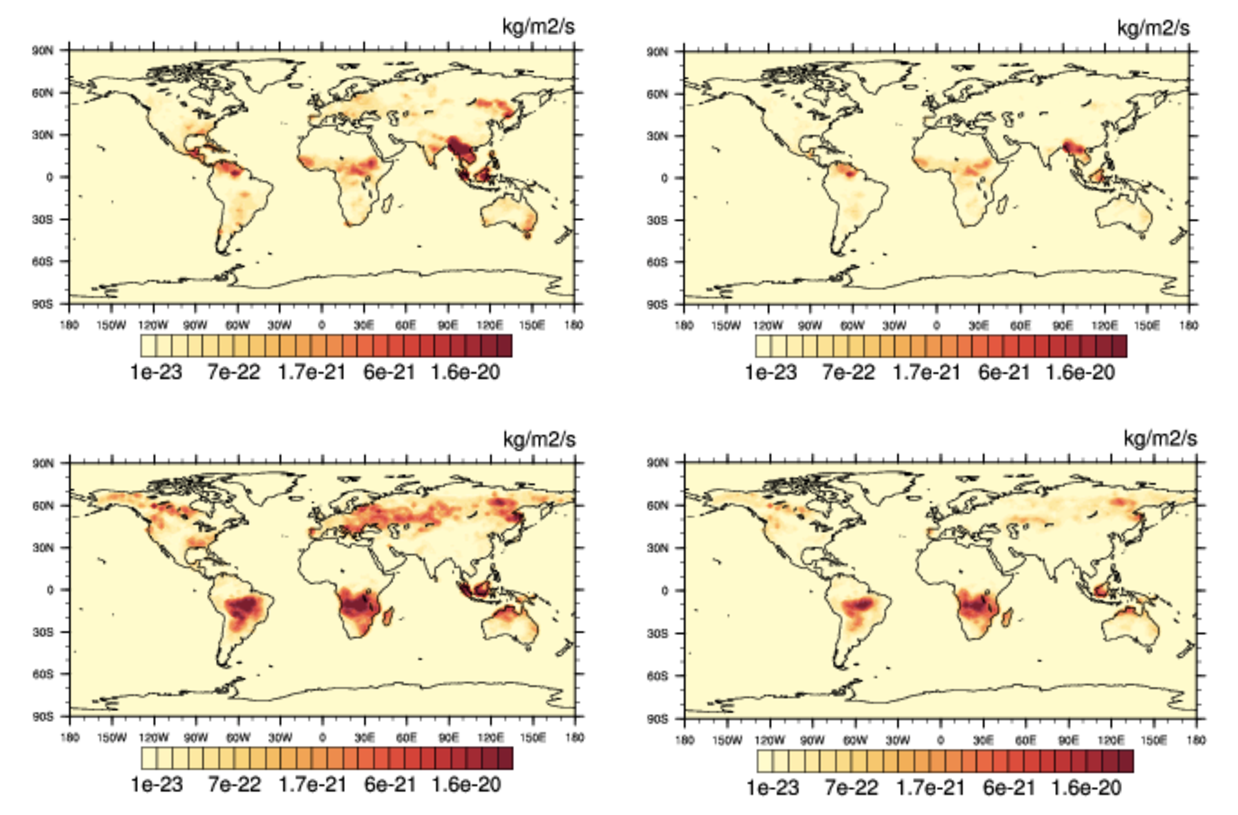
\includegraphics[width = 0.9\textwidth]{Figure12}
				\caption[Monthly mean forest fire and grass fire fluxes of BC for March (top panels) and September (bottom panels), at heights of 0--126~m (left panels) and 278--454~m (right panles)]{\label{fig_P12} Monthly mean forest fire and grass fire fluxes of BC for March (top panels) and September (bottom panels), at heights of 0--126~m (left panels) and 278--454~m (right panels).}
			\end{center}
		\end{figure}
		
		\begin{figure}[h] 
			\begin{center}
				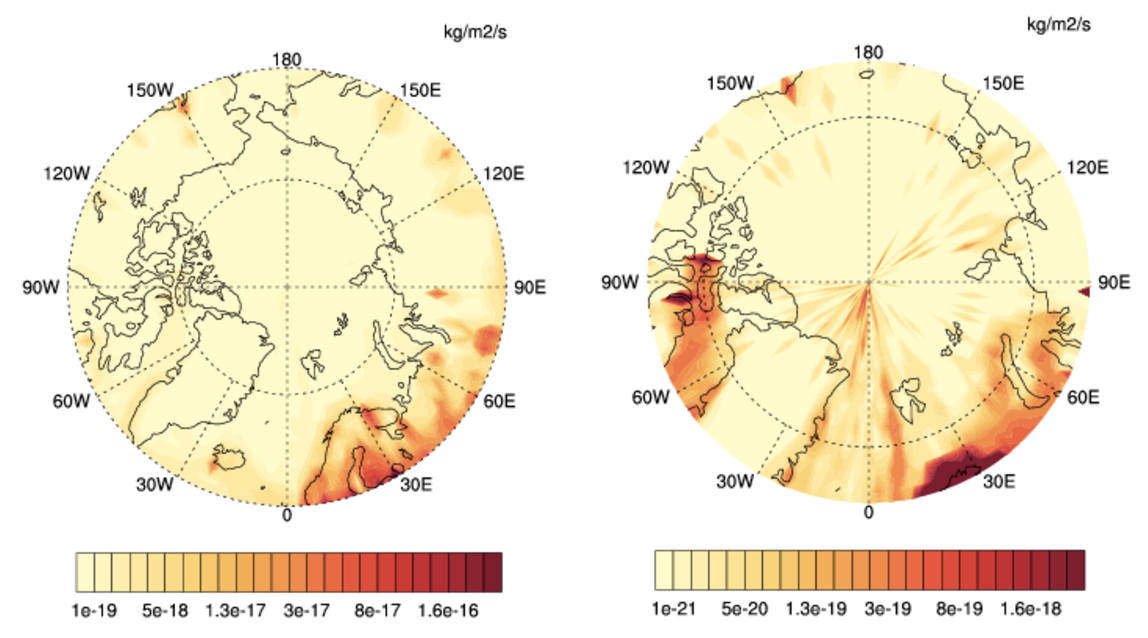
\includegraphics[width = 0.8\textwidth]{Figure11}
				\caption[Annual mean anthropogenic emissions of BC emitted at the surface for the year 2010 for 60--90~$^\circ$N (left) and 70--90~$^\circ$N (right)]{\label{fig_P11} Annual mean anthropogenic emissions of BC emitted at the surface for the year 2010 for 60--90~$^\circ$N (left) and 70--90~$^\circ$N (right).}
			\end{center}
		\end{figure}
		
	
	The model treats hydrophobic BC and hydrophilic BC as two separate species, and all the freshly emitted BC falls into the first category. MAM assumes lognormal size distributions for each mode by setting a fixed standard deviation, and the geometric mean diameter and the total number concentration in each mode can evolve with time. In MAM3, all BC particles are assumed to be aged instantly and put directly into the accumulation mode, where particles are exposed to in-cloud and below-cloud wet deposition. In our study, we applied the newly developed MAM4 model, where the freshly emitted BC/POM particles will come directly into the hydrophobic primary carbon mode. The hygroscopicity of BC is set to be 0, and the hygroscopicity of POM is set to be 0.10, allowing them to experience some in-cloud scavenging in the primary carbon mode. After the aging process due to condensation of sulfate aerosols, ammonia and some semi-volatile organic aerosols and inter-mode or intra-mode coagulation, the fresh carbonaceous particles can be transferred from the primary carbon mode to the accumulation mode, viewed as being aged. A schematic of aerosol modes and associated tracers in MAM4 is shown in Figure~\ref{fig_P1}.
	\begin{figure}[h] 
		\begin{center}
			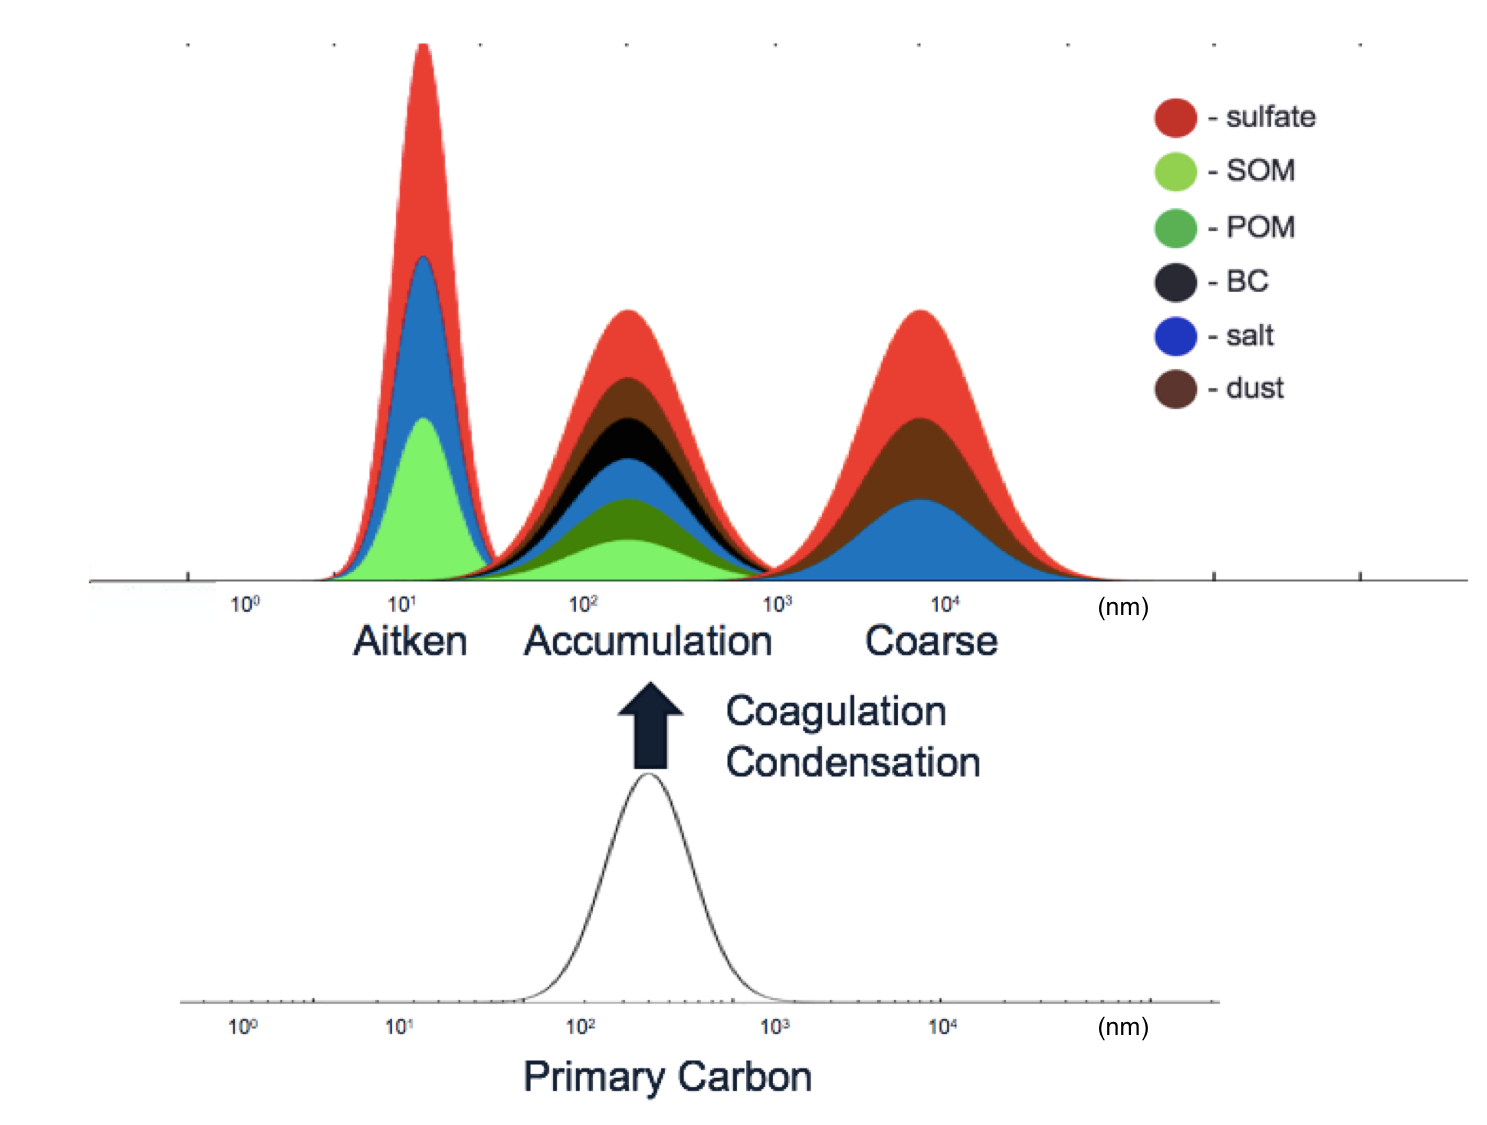
\includegraphics[width = 0.9\textwidth]{Figure01}
			\caption[Schematic of aerosol modes and associated tracers in MAM4]{\label{fig_P1} Schematic of aerosol modes and associated tracers in MAM4.}
		\end{center}
	\end{figure}
	
	
	\section{Eight-monolayer of Sulfate Condensation Criterion}\label{sec_2}
		
	In MAM4, condensation of sulfate, ammonia and semi-volatile organics to carbonaceous particles are treated in a dynamic way, where a ``monolayer condensation criterion" is applied. It assumes that BC particles become hydrophilic after condensing a equivalent of eight-monolayer of sulfate onto its core surface, and then this total mass will be transferred from the primary carbon mode to the accumulation mode based on the standard mass transfer expressions, regarded as being aged \citep{Liu2012}. A schematic of the eight-monolayer condensation criterion is shown in Figure~\ref{fig_P3}. The depth of one monolayer of sulfate is equal to the molecular diameter of sulfate particle ($4.76\times 10^{-10}$~m). It needs to be noted that MAM4 does not track individual particles but instead simulate the evolution of the population distribution in each mode. We will show in Chapter~\ref{sec_1} that the simulated BC concentration and direct radiative forcing are sensitive to the choice of the aging criterion.
	\begin{figure}[h] 
		\begin{center}
			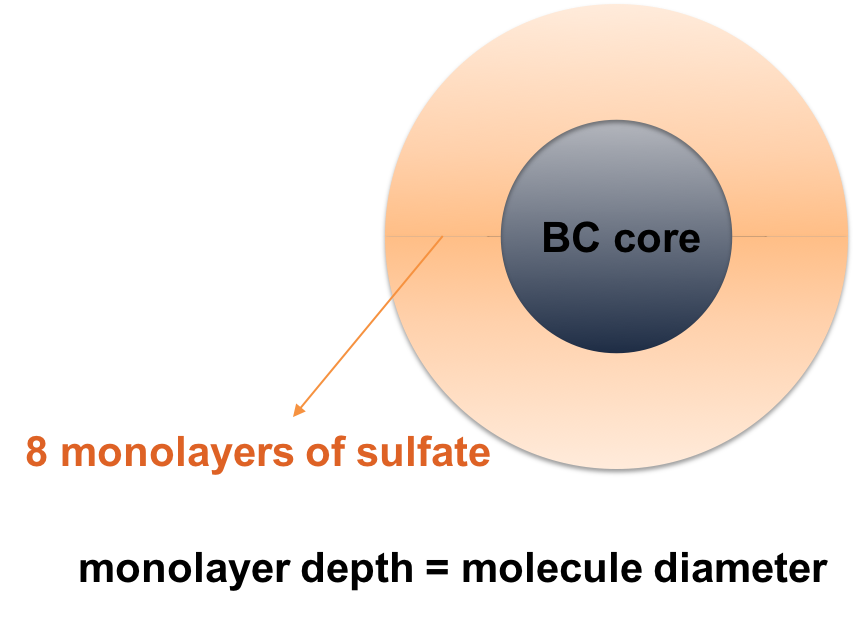
\includegraphics[width = 0.5\textwidth]{Figure03}
			\caption[Schematic of eight-monolayer of sulfate criterion]{\label{fig_P3} Schematic of eight-monolayer of sulfate criterion.}
		\end{center}
	\end{figure}
	
	Currently, the condensation of sulfate and ammonia is assumed to be irreversible, whereas the condensation of semi-volatile organics (SOA) can be set to be reversible or irreversible. Sulfate is produced either from $\rm{SO}_{2}$ oxidation by OH, based on MOZART treatment or from aqueous oxidation by ozone and $\rm H_{2}O_{2}$ \citep{tie2001effects}. An accommodation coefficient (0.65), that is the probability of sticking when the gas molecules encounters the surface of an aerosol particle is used for all the three species \citep{Liu2012}. 
	
	Generally, for each time-step, the model computes the ratio of the condensed soluble species mass in the primary carbon to the mass that is required to age all the particles in that mode based on the monolayer criterion. Then it assumes that the same ratio of the POM and BC in the primary carbon mode is transferred to the accumulation mode together with the condensed materials. Here we provide a detailed mathematical explanations of this model representation of the condensation scheme. 
	
	For mode $n$, the rate of gas uptake $F_{n}$ ($s^{-1}$) is represented as:
	\begin{equation}
	F_{n} = \int n(\text{ln}D_{\rm{p}})\times C d(\text{ln}D_\text{p}) ,
	\end{equation}
	where $D_\text{p}$ is the diameter of the aerosol particles in that mode, $n(lnD_\text{p})$ is the lognormal size distribution, and $C$ is the gas condensation rate (taking sulfuric acid for example):
	\begin{align}
	C = 2\pi \times D_\text{p} \times V_{\rm{diff}} \times F(K_{n}, A) ,\\
	V_{\rm{diff}} = 0.557 \times 10^4 \times 1.75 \times \frac{T}{P}, 
	\end{align}
	
	
	\begin{flushleft}
		$K_{n}$ : Knudsen number, \\
		$A$ : accommodation coefficient, \\
		$F$ : Fuchs-Sutugin correction factor, \\
		$V_{\rm{diff}}$ : gas diffusivity for  $\rm{H_2SO_4}$.
	\end{flushleft}
	The rate of total gas uptake $F_{\rm{sum}}$ is hence estimated by summing up $F_{n}$ over all 4 modes, and the fraction of gas mixing ratio going to each mode $f_{n}$ is equivalent to the ratio of $F_{n}$ to $F_{\rm{sum}}$:
	\begin{align}
	F_{\rm{sum}}  &= \sum_{k=1}^4 F_{n},         &
	f_{n}          &= \frac{F_{n}}{F_{\rm{sum}}}. 
	\end{align}
	
	With the above information, the fraction of soluble species condensing on aerosols during $\Delta t$ is derived as $(1 - e^{-\Delta t\times F_{\rm{sum}}})$, the mass mixing ratio is represented as $q$, and the mass mixing ratio of gas uptake that actually going to mode $n$ during one time-step $\Delta t$ is:
	\begin{equation}
	\Delta q_{n} = q \times f_{n} \times (1 - e^{-\Delta t\times F_ {\rm{sum}}}).
	\end{equation}
	
	The model computes the fraction of carbonaceous aerosols being aged $f_{\rm{age}}$ as the ratio of the volume of actually condensed materials $V_\text{shell}$ to the volume of soluble species required to age all the particles in the primary carbon mode $V_{\rm{8-mono}}$:
	\begin{align}
	\begin{split}
	V_{\rm{shell}} &=  \Delta q_{\rm{SO_4}, n_{\rm{pc}}} \times V_{\rm{SO_4}} \\
	&+ \Delta q_{\rm{NH_4}, n_{\rm{pc}}} \times V_{\rm{NH_4}} \\
	&+ \Delta q_{\rm{SOA}, n_{\rm{pc}}} \times V_{\rm{SOA}}, 
	\end{split}
	\end{align}
	
	\begin{align}
	\begin{split}
	V_{\rm{8-mono}} = \pi M_2 \times d_{\rm{8-mono}},
	\end{split}
	\end{align}
	
	\begin{align}
	f_{\rm{age}} &= \frac{V_{\rm{shell}}}{V_{\rm{8-mono}}},  
	\end{align}
	
	\begin{flushleft}
		$V_{\rm{SO_4}}$, $V_{\rm{NH_4}}$, $V_{\rm{SOA}}$: factors that convert the unit of mixing ratio to $m^3/$kmol air. \\
		$V_{\rm{8-mono}}$: the volume of sulfate required to age all BC particles. \\
		$M_2$, $M_3$: second and third moment of  moment dynamic equation, $\pi M_2/ \frac{\pi}{6}M_3$ is the ratio of aerosol surface area to volume. \\
		$d_{\rm{8-mono}}$: the thickness of eight monolayers of sulfate.
	\end{flushleft}
	
	The changes of mass in each mode over $\Delta t$ are then represented as:
	\begin{align}
	\Delta q_{n_{\rm{pc}}} &= \Delta q_{n_{\rm{pc}}} - f_{\rm{age}} \times q_{n_{\rm{pc}}}  &&\text{primary carbon mode}, \\
	\Delta q_{n_{\rm{accu}}} &= \Delta q_{n_{\rm{accu}}} + f_{\rm{age}} \times q_{\rm{n_{\rm{pc}}}}  &&\text{accumulation mode}.
	\end{align}
	
		\section{BC Mass Fraction Activated by Coating Material}
		CAM-chem MAM4 assumes that the hydrophobic BC particles in  primary carbon mode will be activated and transferred to the accumulation mode after condensing a certain number of sulfate molecular layers, and it uses eight monolayers as default. The size and hygroscopicity of BC aerosols will be increased as more condensible material is coated onto their surface, and this will lead to a decreasing supersaturation ratio to activate the particles. In MAM4, more coating material is required to age BC for larger number of monolayers, so the critical supersaturation ratio will be decreases for a larger number of monolayers. \citet{Liu2012} has estimated the critical supersaturation for three and eight monolayers of sulfate to produce CCN from BC aerosols, and the values are 0.49$\%$ and 0.32$\%$ respectively. 
		
		Following Liu at al. (2012), we derived similar results and the values are 0.43$\%$ and 0.28$\%$ for three and eight monolayers respectively. Furthermore, we computed the fraction of BC mass that can be activated at a certain specific supersaturation ratio based on K{\" o}hler Equation. In our estimation, we assume that BC cores follow a lognormal size distribution with a fixed standard deviation ($\sigma$=1.4) and a changeable mean diameter ranging from 80 to 150~nm considering the fact that the volume mean size for BC and POM emissions is 134~nm. The number of monolayers ranges from 1 to 23 to cover a wide range of choices. The hygroscopicity value for sulfate is 0.65, and the thickness of one sulfate monolayer is $4.76 \times 10^{-10}$~m. Figure~\ref{fig_P10} shows the results at supersaturation ratios of 0.3~$\%$ and 0.6~$\%$ since those values are typical for cloud regimes ranging from stratiform to cumulus clouds. For non-hygroscopic particles whose sizes follow the lognormal distribution with a mean diameter of 134~nm, condensing eight monolayers of sulfate can activates 65.9~$\%$ and 99.5$\%$ of BC mass with critical supersaturations of 0.3~$\%$ and 0.6~$\%$, respectively.  
		
		\begin{figure}[h] 
			\begin{center}
				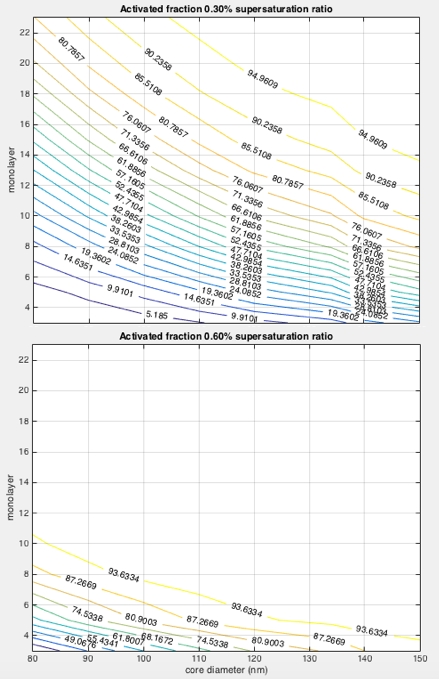
\includegraphics[width = 0.6\textwidth]{Figure10}
				\caption[Fraction of BC mass that is activated at 0.3$\%$ (top) and 0.6$\%$ (bottom) supersaturation ratio]{\label{fig_P10} Fraction of BC mass that is activated at 0.3$\%$ (top) and 0.6$\%$ (bottom) supersaturation ratio.}
			\end{center}
		\end{figure}
	\section{CAM-chem Aging Timescale}
	Using a first-order aging model, the transition of BC mass from the fresh to the aged mode can be represented by an aging timescale. The model is given by
	\begin{align}\label{eq:12}
	\frac{dM_{\rm{fresh}}}{dt} = -\frac{1}{t_{\rm{aging}}}M_{\rm{fresh}}. 
	\end{align}
	Here, $M_{\rm{fresh}}$ is the mass of freshly emitted BC particles.
	Rearranging equation~\ref{eq:12}, we can represent the aging timescales as the production of the inverse of the mass transfer rate and the fresh BC mass: 
	\begin{align}\label{eq:9}
	t_{\rm{aging}} = M_{\rm{fresh}}/(-\frac{dM_{\rm{fresh}}}{dt}).
	\end{align}
	Any particle transition from the fresh to aged mode during a time step is either by coagulation with other particles or by accumulating a certain amount of condensable materials. So the overall aging timescale $t_{\rm{aging}}$ can be represented as the combination of the aging timescales by condensation $t_{\rm{cond}}$ and by coagulation $t_{\rm{coag}}$:
	\begin{align}\label{eq:10}
	\frac{1}{t_{\rm{aging}}} =\frac{1}{t_{\rm{coag}}} + \frac{1}{t_{\rm{cond}}}.
	\end{align}
	Each of the component aging timescales $t_{\rm{cond}}$ and $t_{\rm{coag}}$ can be derived from the corresponding mass transfer rate by applying Equation~ \ref{eq:9}. 
	
	In CAM-chem model, BC particles are transferred from the fresh, primary carbon model to the aged, accumulation mode according to mass transfer rates computed from the coagulation and condensation processes, respectively. We extracted the mass transfer rates every 6 hours and applied Equation~(\ref{eq:9}) and Equation~(\ref{eq:10}) to obtain the corresponding timescales for aging. We are able to evaluate the contribution of condensation and coagulation to the overall aging by showing their  timescales separately. In this study, we evaluated the monthly and annually averaged aging timescales. 
	
	\section{PartMC-MOSAIC Aging Timescale}\label{sec_4}
	PartMC-MOSAIC (particle resolved model) can track the evolution of individual particles as they evolve through condensation, coagulation, emission and evaporation of SOA \citep{riemer2009simulating}. It has the advantage in simulating BC aging that no specific criterion assumption is required. In a previous study, \citet{Fierce2016} has investigated a reduced representation of mixing state for simulating aerosol effects on climate. The mixing timescales that characterized this transformation have been parameterized. In our study, we applied this aging timescale parameterization to our global models outputs to evaluate the accuracy of our global model aging timescales.
	
	The following summarizes the procedure that was applied in \citet{Fierce2016} to obtain the aging timescale parameterization. \citet{Fierce2016} simulated a series of 100 sensitivity particle-resolved scenarios using Latin hypercube sampling to sample the parameter space of the model inputs \citep{mckay1979comparison}. Twenty-eight input parameters were varied to represent a range of atmospheric conditions, from highly polluted cases with consequently rapid aging to remote regions with slow aging. Those parameters included environmental variables, aerosol characteristics, aerosol type and gas emissions. In each scenario, they simulated the evolution of carbonaceous particles that were emitted into a population of background aerosol. No new fresh particle were emitted during this process after the simulation started, in order the isolate the effects of aging \citep{Fierce2016}. The normalized error in the number concentration of CCN computed using the particle-resolved composition that track individual particle and the reduced representation of the composition by assuming different mixing states of aerosol population for a specific scenario $q$ at time $t$ is given by:
	\begin{align}\label{eq:11}
	e_{\rm CCN}(t) = \frac{\int_{0}^{\infty}( \tilde{N}_{\rm CCN}(t,s) - 
		N_{\rm CCN} (t,s))ds}{\int_{0}^{\infty} N_{\rm CCN, q}(t,s)ds},
	\end{align}
	where $\tilde{N}_{\rm CCN}(t,s)$ is the number concentration of CCN using the reduced composition at a specific environmental supersaturation $s$ and time $t$, and $N_{\rm CCN}(t,s)$ is the CCN using the particle-resolved composition. This error decreases exponentially with time and a regression result has shown a high $R$-squared value as 93$\%$. The equation can be expressed as:
	\begin{align}
	e_{\rm CCN}(t) = e_{\rm CCN}(t_{0})\text{exp}(-\int_{t_{0}}^{t}\frac{1}{\tau_{\rm mix}(t)} dt), 
	\end{align}
	where $\tau_{\rm mix}$ is the overall aging timescale. 
	A particle is either aged by condensation or by coagulation, so the two processes can be treated as separate process and has their own timescale \citep{Fierce2015}. Accordingly, the overall timescale is found to be a function of the condensation growth rate $I(t)$ and the particle number concentration $N(t)$.
	So a more specified parameterization of $\tau_{\rm mix}$ can be derived by regression of the error on $I(t)$ and $N(t)$:
	\begin{align}
	e_{\rm CCN}(t) = e_{\rm CCN}(t_{0})\text{exp}(-k_{\rm cond}\int_{t_{0}}^{t} I(t) dt)\text{exp}(-k_{\rm coag}\int_{t_{0}}^{t}N(t) dt), 
	\end{align}
	Figure~\ref{fig_P2} is an example of determining $k_{\rm coag}$ after setting $I(t)$ to be 0. 
	
	The PartMC-MOSAIC parameterized aging timescales can then be represented as:
	\begin{align}
	\tau_{\rm overall} \approx (k_{\rm cond}I_{\rm cond} + k_{\rm coag}N)^{-1},
	\end{align}
	
	\citet{Fierce2016} has shown the estimated e-folding time $\tau_{\rm overall}$ computed from the approximate range of condensation growth rate and number concentration for specific locations (Figure~\ref{fig_P7}). This range can also be used an a reference for global models. 
	
	In our study, we computed the number concentration $N$ as the sum of the particle number concentration of all modes, and the condensation growth rate $I$ as the volume condensation rate over the total aerosol surface area. As is mentioned in 3.2, the condensation of SOA is reversible, so the total condensation rate can be positive or negative. Since all fresh BC particles are in the primary carbon mode, we computed the condensation growth rate using the volume condensation rate and surface area extracted from the primary carbon mode. 
	
	\begin{figure}[h] 
		\begin{center}
			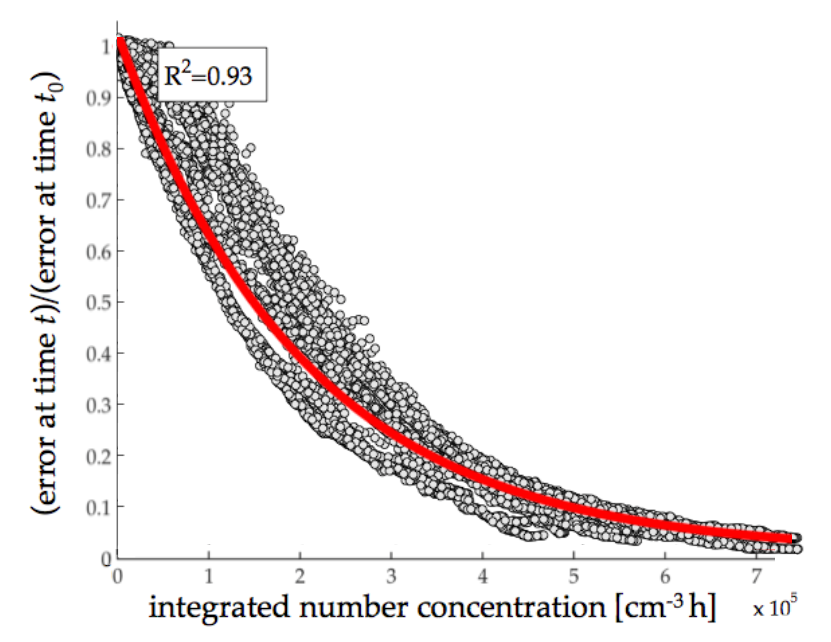
\includegraphics[width = 0.6\textwidth]{Figure02}
			\caption[Raw data that is used to construct the regression function (grey dots) and the resulting regression function (black line) for simulations including only coagulation, without condensation \citep{Fierce2016}]{\label{fig_P2}Raw data that is used to construct the regression function (grey dots) and the resulting regression function (black line) for simulations including only coagulation, without condensation \citep{Fierce2016}.}
		\end{center}
	\end{figure}
	
	\begin{figure}[h] 
		\begin{center}
			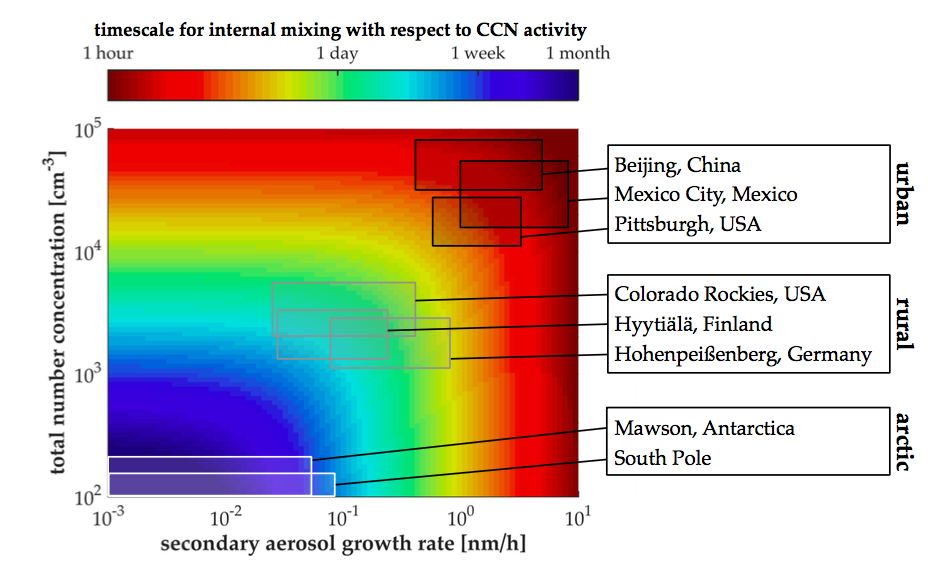
\includegraphics[width = 0.8\textwidth]{Figure07}
			\caption[Estimated e-folding time for the error in CCN activity from the internal mixture approximation. \citep{Fierce2016}]{\label{fig_P7}Estimated e-folding time for the error in CCN activity from the internal mixture approximation. \citep{Fierce2016}.}
		\end{center}
	\end{figure}
	
	\clearpage
	
	\chapter{Results}
	In this chapter, we will show the sensitivity of BC burden and radiative forcing to the choices of CAM-chem aging parameters. Also, we will assess the mixing states of the species in CAM-chem model and furthermore, BC mass fraction and mixing states that can be captured by SP2 measurements. Finally, the process analysis of BC aging will be discussed.
	
	\section{Sensitivity of BC Burden and Radiative Forcing to the Aging Criterion}{\label{sec_1}}
	To explore the model sensitivity to the aging criterion (see Chapter~\ref{sec_2}), we conducted four experiments at a resolution of $1.9^\circ \times 2.5^\circ$ from January 1 2010 to December 31 2010 with offline meteorology, and set the number of mono-layers to 1, 2, 4 and 8 (default), respectively, abbreviated as L1, L2, L4 and L8. The larger the number of monolayer is, the more coating material is required to transfer the carbonaceous aerosols from the primary carbon mode to the accumulation mode, hence BC will stay longer in the primary carbon mode and the aging rates will be slower. Consequently, the BC concentration will be higher because less BC is transferred to the hydrophilic, accumulation mode that is subject to wet deposition. 
	\subsection{Horizontal Distribution of BC burdens}
	Figure~\ref{fig_P13} shows the horizontal distributions of BC mixing ratio near the surface in the L8 case (top panel), and the relative differences between L1 and L8 cases (bottom panel), denoted by (L1 - L8)/L8. Generally, BC concentrations are highest in east Asia and lowest in the Arctic Region, ranging from 0 to 1000 ng/kg. BC concentrations in the L1 case are lower than L8 case throughout the globe with maximum differences in the annually averaged BC mixing ratio of 16$\%$ near the surface. This is because the aging is faster with a smaller threshold of the number of monolayers, and hence fresh BC will be transferred to the accumulation mode more quickly. The accumulation mode aerosols are then subject to wet removal, which will prevent them from traveling to remote regions.     
	
	We observed that the relative differences increase as BC is transported away from the source regions, such as the South Atlantic Ocean downwind of Center Africa or the North Pacific near Southeast Asia. Both show higher differences than their surrounding regions and can be matched to an obvious BC burden gradient along the plumes of BC over the ocean. The simulated BC burden is most sensitive to the choices of the aging criterion in the high-latitude regions where the background concentrations are low, with maximum differences in the annually averaged BC mixing ratio of 16$\%$ near the surface. This is because the longer distance BC travel, the more BC in the accumulation mode will be subject to wet deposition. Considering that BC is transferred to the accumulation mode less quickly in the L8 case, the relative difference of BC concentrations between L1 and L8 cases tend to be higher in distant regions.
	
	Similarly, Figure~\ref{fig_P21} shows the horizontal distributions of BC mixing ratio (L8) the relative differences between the L1 and L8 cases for March and September. We can observe clear seasonal variability of BC mixing ratios (top panels) most probably due to the differences in their emission sources. For example, as is mentioned before, more biomass burning combustion can be observed in South Africa and South America in September. This can contribute to the high-concentration plumes in those regions in September compared to March. The different patterns in the meteorology fields can also be another contribution.
	
	\begin{figure}[h] 
		\begin{center}
			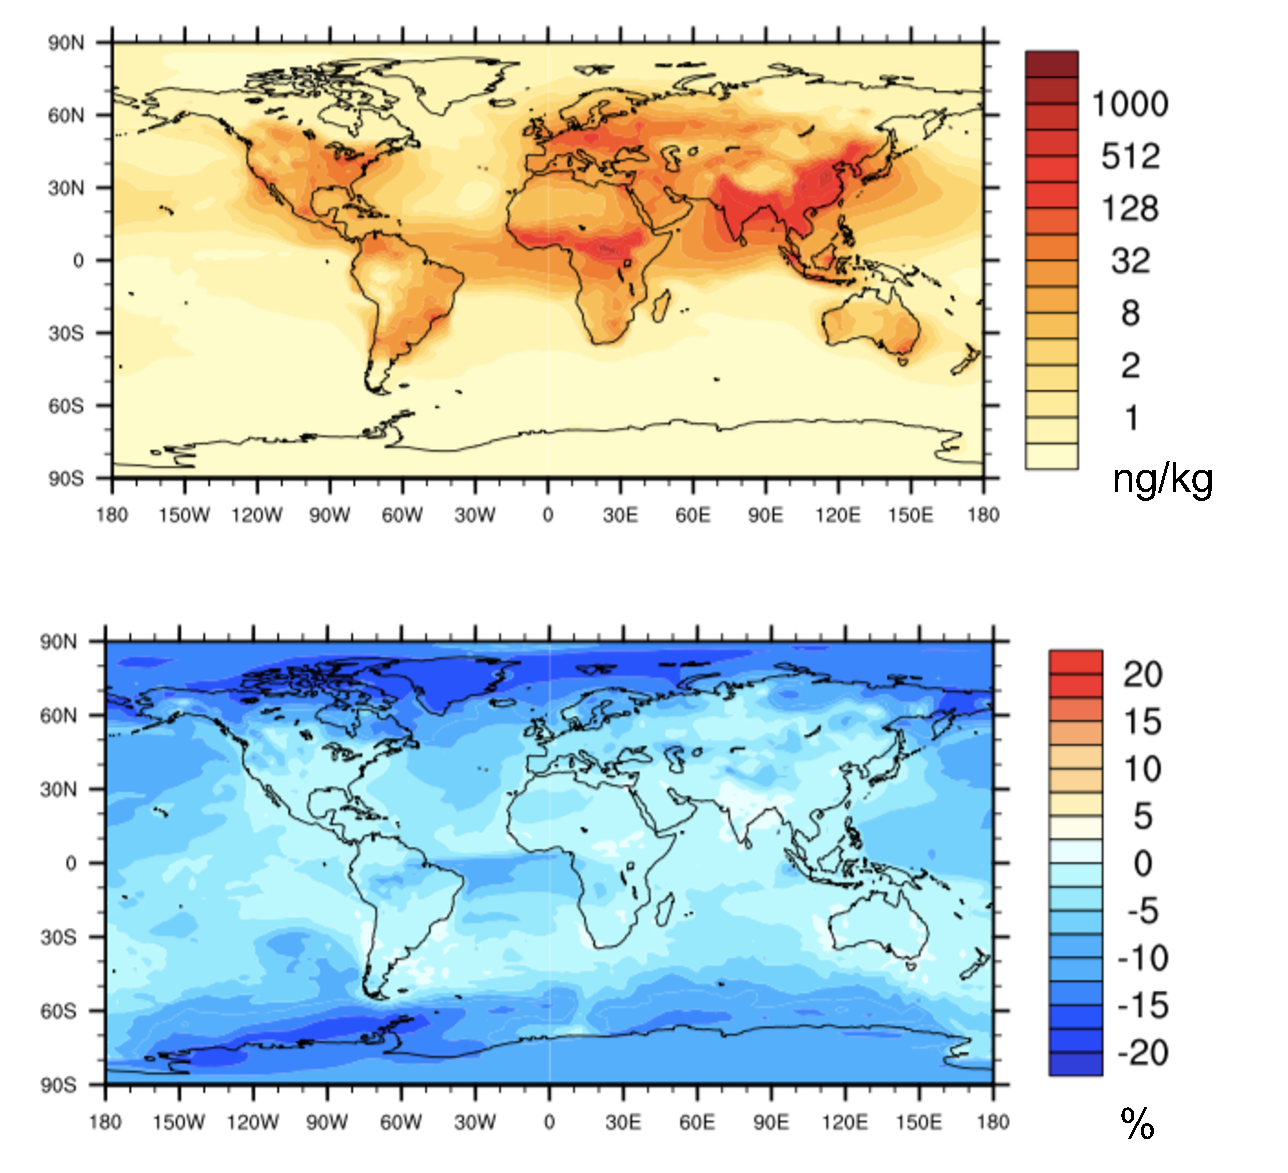
\includegraphics[width = 0.6\textwidth]{Figure13}
			\caption[Annually averaged BC mass mixing ratio (top) and relative differences denoted by (L1 - L8)/L8 (bottom)]{\label{fig_P13} Annual BC mass mixing ratio (top) and relative differences between the cases L1 and L8, denoted by (L1 - L8)/L8 (bottom).}
		\end{center}
	\end{figure}
	
	\begin{figure}[h] 
			\begin{center}
				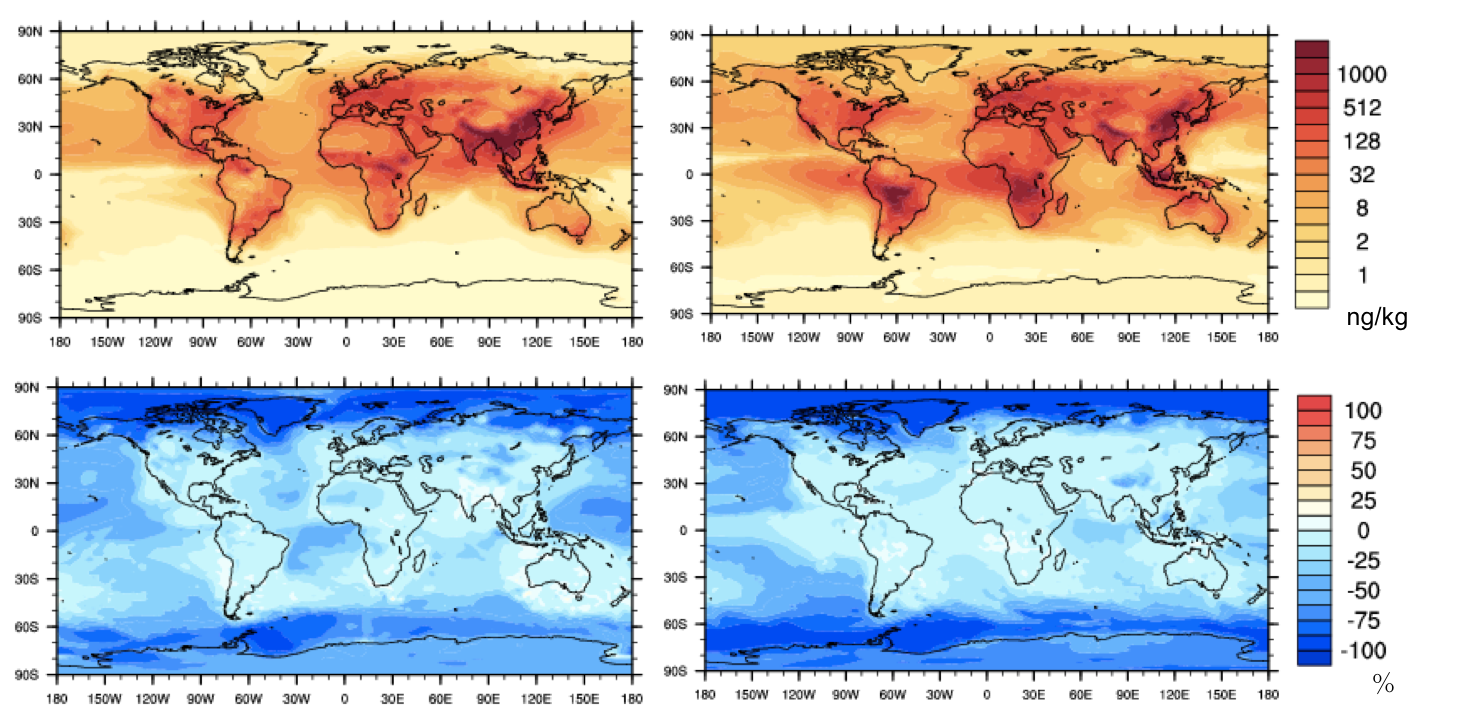
\includegraphics[width = 1\textwidth]{Figure21}
				\caption[Monthly averaged BC mass mixing ratio (top) and relative differences denoted by (L1 - L8)/L8 (bottom) near the surface for March (left) and September (right).]{\label{fig_P21} Monthly averaged BC mass mixing ratio (top) and relative differences denoted by (L1 - L8)/L8 (bottom) near the surface for March (left) and September (right).}
			\end{center}
		\end{figure}
	
	\subsection{Vertical Profiles of BC burdens}\label{sec_8}
	Figures~\ref{fig_P14} and \ref{fig_P16} show the sensitivity of BC vertical distributions to the number of monolayers in six regions (Figure~\ref{fig_P15}). Region 1 and 2 are distant from emission sources while the other four regions are dominated either by biomass burning activities (region 3 and 4) or by emissions from both anthropogenic and biomass burning activities (region 5 and 6). Throughout the source regions, a decreasing trend of BC burdens with height is shown whereas an increasing trend is observed instead for distant regions, probably due to the wet removal process that prevents lower level BC from being transported far away from its sources. These results are still to be further evaluated in the future, considering that the model simulations tend to overestimate BC burdens in the upper troposphere and underestimate BC burdens at altitudes below 400 hPa \citep{Liu2016}. It is obvious that BC distributions in distant regions are more sensitive to the number of monolayers (region 1 and 2 compared to 3--6). The maximum relative differences (71~$\%$) among the six regions are found at 400 hPa in region 2 during March, indicating that the highest model sensitivity can appear at high altitudes near the Arctic. 
	
	Figure~\ref{fig_P14} and \ref{fig_P16} also compare the model-simulated BC vertical profiles in March and September in order to explore their seasonal variability. Regions dominated by biomass burning have significant increases of BC burdens in September by one order of magnitude (regions 3 and 4). BC mixing ratios tend to be maximum in September because of South American and Africa biomass burning activities in the dry season \citep{Liu2016}. The poleward transport can also be seen from the vertical profile of region 1 at high altitudes above 400~hPa, especially for September. The differences among the four MAM4 experiments are smaller in September especially in the Arctic and oceanic regions. In addition, more BC are concentrated in the upper troposphere in September, probably because of the biomass burning activities produces BC at higher altitudes compared to other sources. 
	
	\begin{figure}[h] 
		\begin{center}
			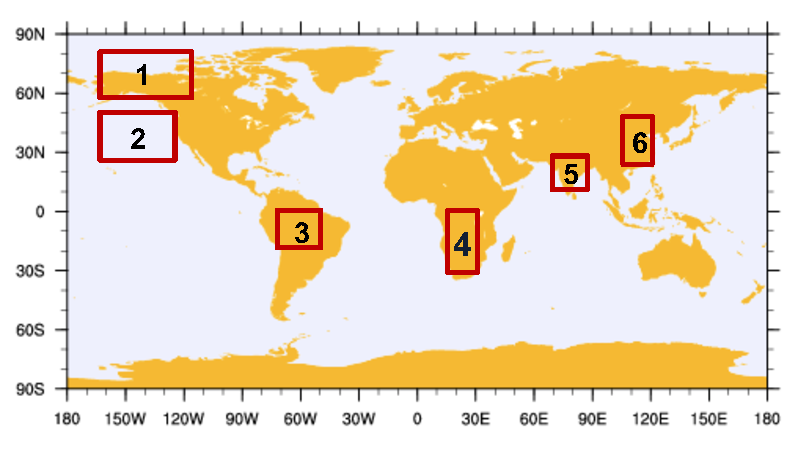
\includegraphics[width = 0.5\textwidth]{Figure15}
			\caption[Horizontal map of six regions]{\label{fig_P15} Horizontal map of six regions: Region 1 (162$^\circ$W--112$^\circ$W, 60$^\circ$N--80$^\circ$N), Region 2 (160$^\circ$W--130$^\circ$W, 30$^\circ$N--50$^\circ$N), Region 3 (75$^\circ$W--55$^\circ$W, 10$^\circ$S--1$^\circ$N), Region 4 (15$^\circ$E--30$^\circ$E, 30$^\circ$S--0$^\circ$N), Region 5 (73$^\circ$E--83$^\circ$E, 15$^\circ$N--27$^\circ$N), Region 6 (108$^\circ$E--120$^\circ$E, 23$^\circ$N--43$^\circ$N).}
		\end{center}
	\end{figure}
	
	\begin{figure}[h] 
		\begin{center}
			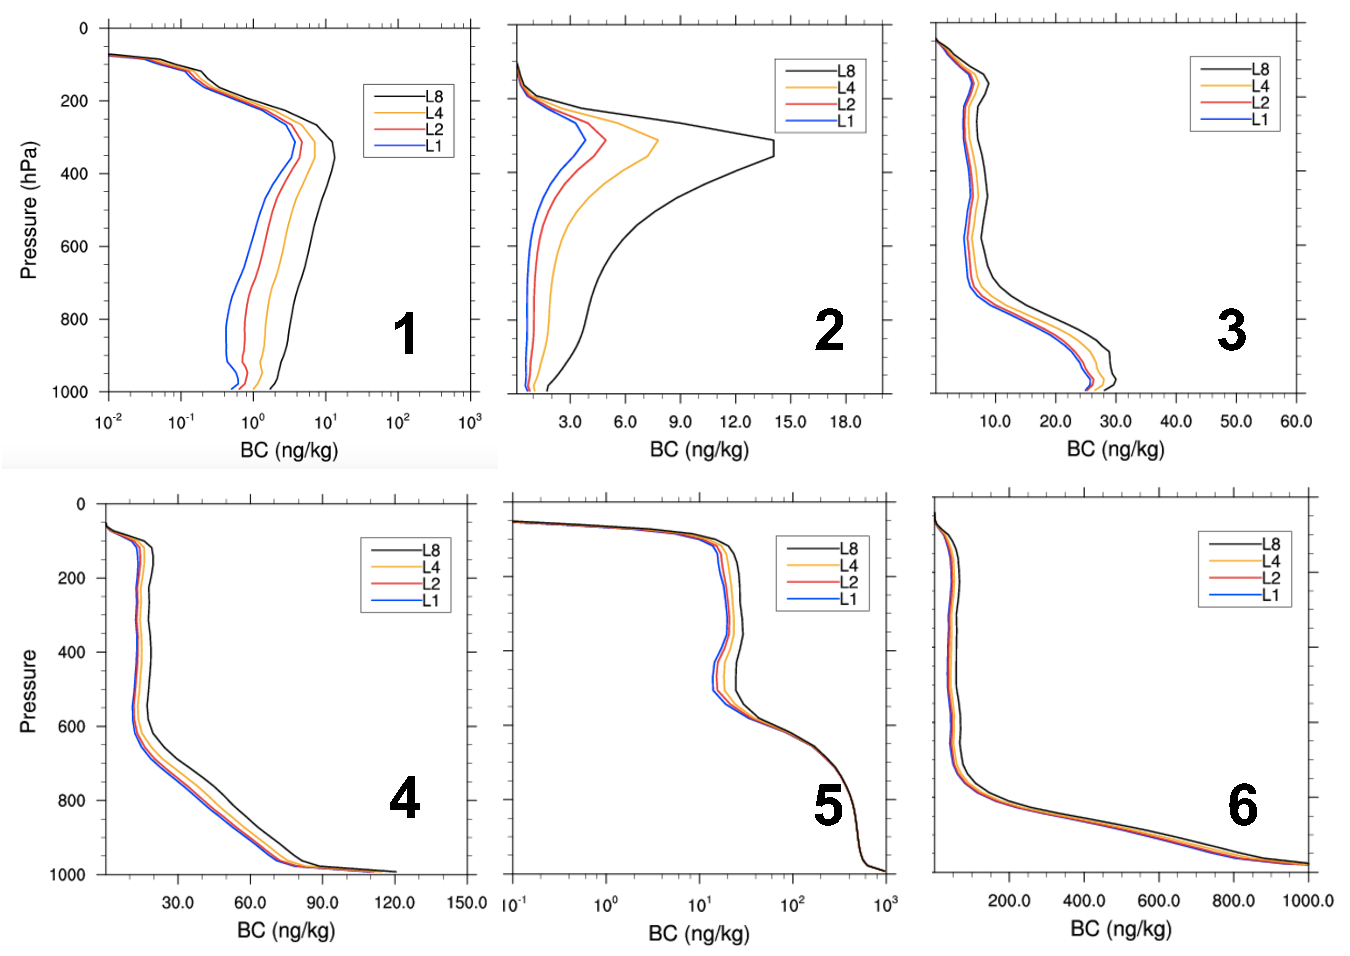
\includegraphics[width = 0.7\textwidth]{Figure14}
			\caption[Vertical profiles of mean  burdens for six regions corresponding to Figure~\ref{fig_P15} in March, 2010]{\label{fig_P14} Vertical profiles of mean  burdens for six regions corresponding to Figure~\ref{fig_P15} in March, 2010.}
		\end{center}
	\end{figure}
	
	
	\begin{figure}[h] 
		\begin{center}
			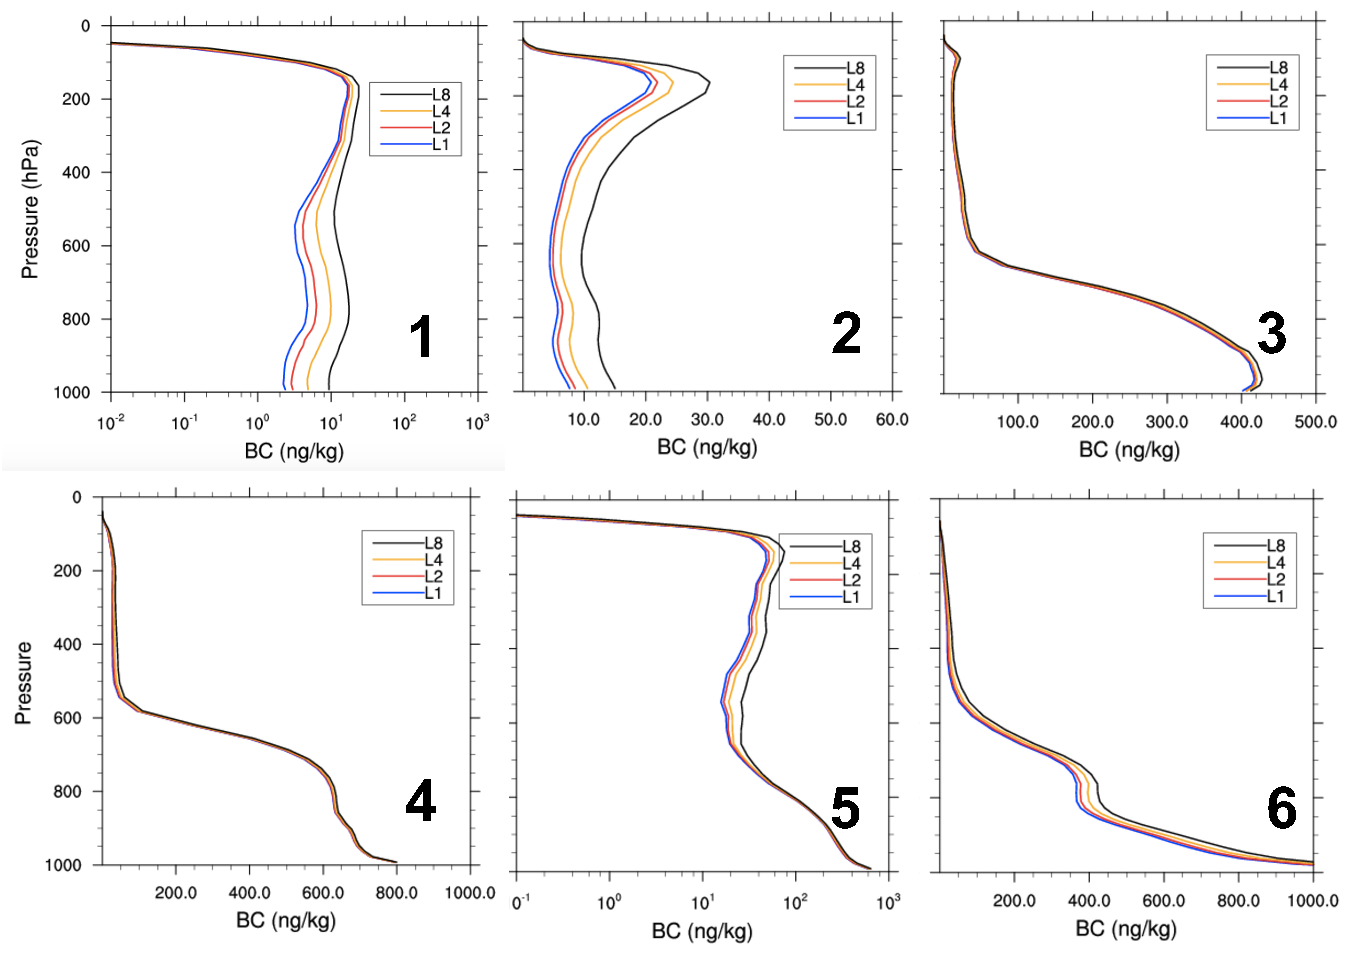
\includegraphics[width = 0.7\textwidth]{Figure16}
			\caption[Vertical profiles of mean BC burdens for six regions corresponding to Figure~\ref{fig_P15} in September, 2010]{\label{fig_P16} Vertical profiles of mean BC burdens for six regions corresponding to Figure~\ref{fig_P15} in September, 2010.}
		\end{center}
	\end{figure}
	
	
	Figure~\ref{fig_P20} shows the horizontal plots of regional BC concentrations at 859~hPa for the arctic region. The BC radiative forcing is very sensitive to BC burden especially in the Arctic region, so it is important to assess the extent to which BC concentrations are sensitive to the aging assumption in the climate model. The patterns of BC distributions in the two MAM4 experiments are quite different, in addition to their regional mean differences among the cases that has been explained in the previous paragraphs. This finding indicates that the sensitivity of not only the magnitude of averaged BC burdens, but also their latitudinal and longitudinal patterns are both very sensitive to the aging criterion, especially in the middle and upper troposphere. Understanding the BC aging process so as to improve the reliability of the number-of-monolayer criterion is quite important for the accuracy of CAM-chem MAM4 BC simulations.
	
	
	\begin{figure}[h] 
		\begin{center}
			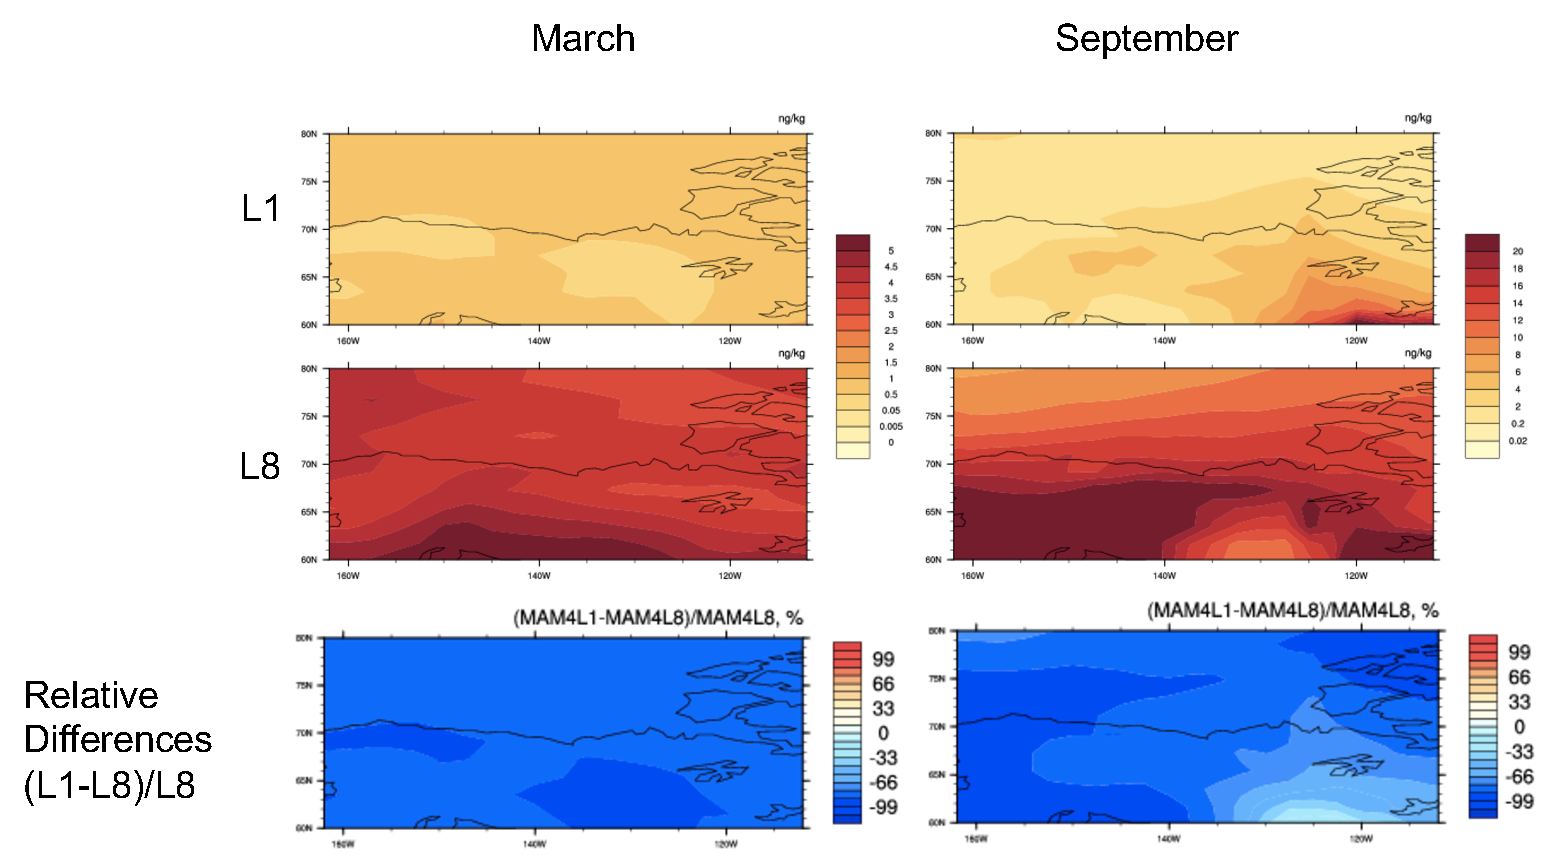
\includegraphics[width = 1\textwidth]{Figure20}
			\caption[Horizontal plots of regional BC concentrations at 859~hPa covering region 1 in case L1 (top) and L8 (middle), and the relative differences (bottom) denoted by (L1 - L8)/L8]{\label{fig_P20} Horizontal plots of regional BC concentrations at 859~hPa covering region 1 in case L1 (top) and L8 (middle), and the relative differences (bottom) denoted by (L1 - L8)/L8.}
		\end{center}
	\end{figure}
	
	\subsection{BC Deposition Flux}
	We also explored the sensitivity of BC deposition flux through both wet and dry processes to the aging criterions, and compared their differences between two cases (L1 v.s. L8). Figure~\ref{fig_P17} and \ref{fig_P18} show the relative differences of the monthly averaged wet deposition rates and dry deposition rates respectively, and compare the seasonal differences. 
	
	\begin{figure}[h] 
		\begin{center}
			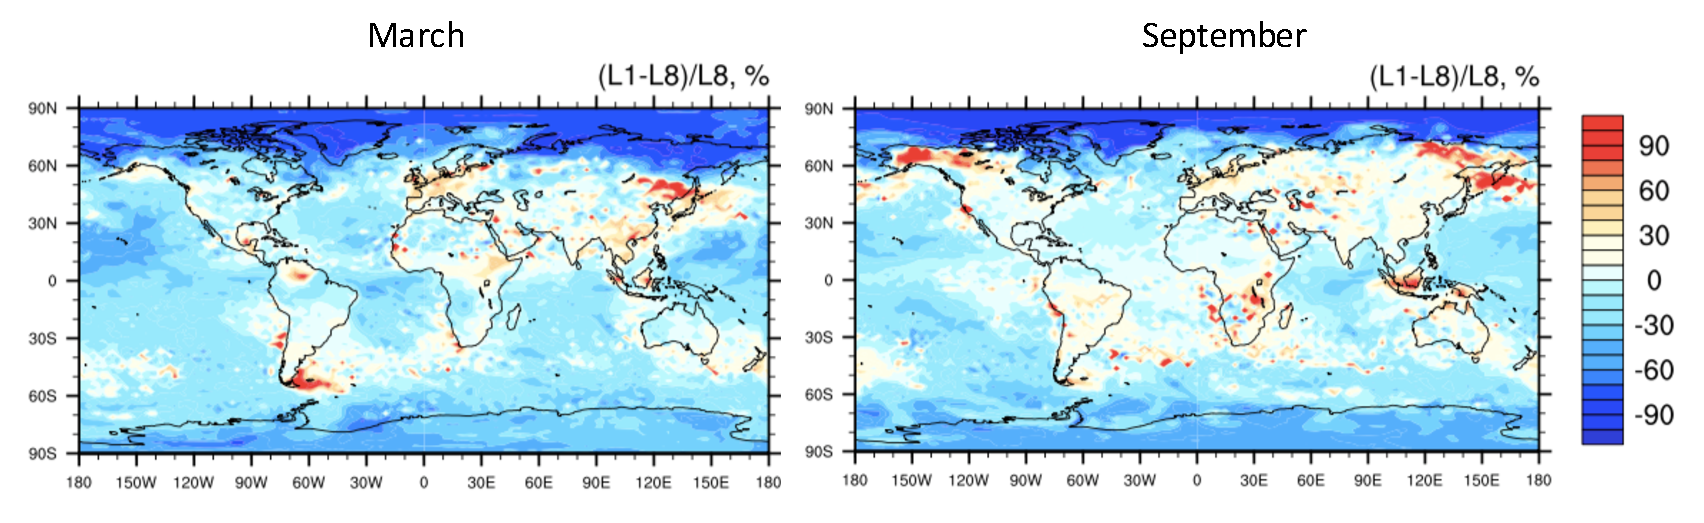
\includegraphics[width = 1\textwidth]{Figure17}
			\caption[Horizontal plots of the relative differences in BC wet deposition flux with different aging criterion (L1 v.s. L8) for March (left) and September (right).]{\label{fig_P17} Horizontal plots of the relative differences in BC wet deposition flux with different aging criterion (L1 v.s. L8) for March (left) and September (right).}
		\end{center}
	\end{figure}
	
	
	\begin{figure}[h] 
		\begin{center}
			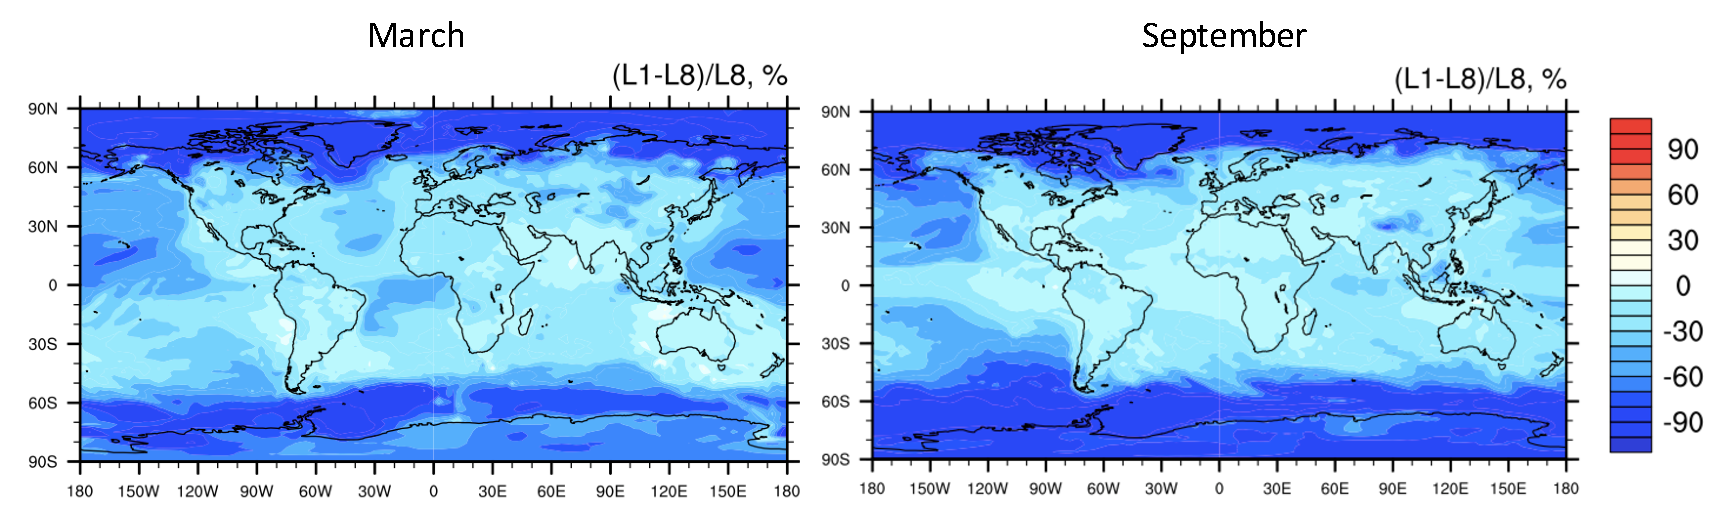
\includegraphics[width = 1\textwidth]{Figure18}
			\caption[Horizontal plots of the relative differences in BC dry deposition flux with different aging criterion (L1 v.s. L8) for March (left) and September (right)]{\label{fig_P18} Horizontal plots of the relative differences in BC dry deposition flux with different aging criterion (L1 v.s. L8) for March (left) and September (right).}
		\end{center}
	\end{figure}
	
	As is expected, the wet deposition rates with a smaller threshold of coating thickness giving to faster aging rates are higher in the main source regions (South East Asia, Europe, South America, Aftica, etc.) by a factor around 4. The wet deposition rates in case L1 become smaller than case L8 in remote regions such as the distant oceans and polar regions, with the highest relative differences attaining 90~$\%$ in the Arctic. This is because BC stays longer in the primary carbon mode with a larger number of monolayer criterion, and hence can be transported to distant regions. We also noticed the high values at the north edge of mainland Russia or at the south edge of South America continent, primarily because of the small values of the background concentrations (the denominator of the relative difference equation).
	
	The dry deposition rates are positively related to the overall number concentration of BC aerosols (Figure~\ref{fig_P21}), where higher concentrations lead to larger dry deposition fluxes. So similarly to our analysis in section~\ref{sec_1}, BC concentrations in L1 case are lower than L8 case throughout the globe, and the relative differences increase along the pathway of BC as it is transported away from the source regions. The dry deposition rates are most sensitive to the choices of aging criterion in the high-latitude regions, with maximum differences of 99$\%$ in the Arctic for September. This is relevant for the deposition of BC on snow and ice.
	
	
	\subsection{Radiative Forcing }
	We analyzed the sensitivity of BC radiative forcing to the aging criterions, and compared their differences between L1 and L8 cases. Figure~\ref{fig_P23} shows the horizontal distribution of the annually averaged direct radiative forcing of black carbon aerosols respectively, and compares the differences between the L1 and L8 cases. It is interesting to note that a consistent band of positive forcing in the L8 case is at very high latitudes, whereas in the L1 case there are mostly negative forcing in the same regions.
	\begin{figure}[h] 
		\begin{center}
			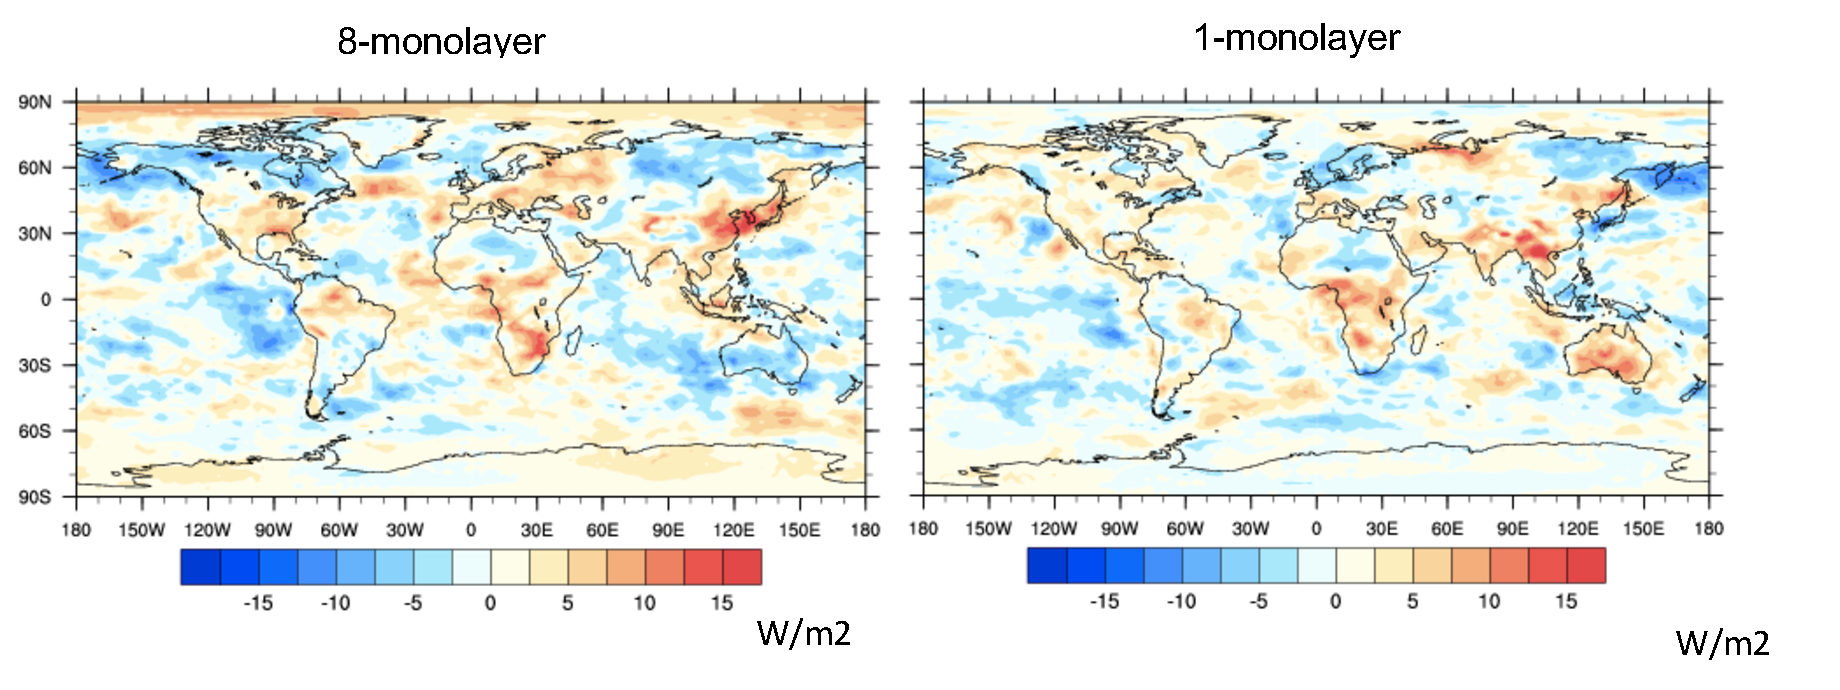
\includegraphics[width = 1\textwidth]{Figure23}
			\caption[Horizontal plots of the direct radiative forcing of BC aerosols with different aging criterion (L1 v.s. L8) near the surface (992hPa)]{\label{fig_P23} Horizontal plots of the direct radiative forcing of BC aerosols with different aging criterion (L1 v.s. L8) near the surface (992hPa).}
		\end{center}
	\end{figure}
	
	
	As shown before, a smaller threshold of coating thickness gives rise to faster aging rates and a larger portion BC in the accumulation mode (internally mixed). The accumulation mode aerosols are subject to wet scavenging and removed as they are transported to distant regions. We have shown in the previous sections that generally BC mixing ratios in the L1 case are lower than L8 case throughout the globe, and the simulated BC burden is most sensitive to the choices of its aging criterion at high latitudes where the background concentrations are low. Consequently, the magnitude of the globally averaged radiative forcing is 0.18~W$\cdot{\text{m}^{-2}}$ in the L1 case, lower than the radiative forcing of 0.48~W$\cdot{\text{m}^{-2}}$ in the L8 case because less BC and consequently faster aging and wet deposition. The magnitudes are higher in the main source regions (South East Asia, Europe, South America, Africa, etc.) with a maximum of around 15~W$\cdot{\text{m}^{-2}}$ in both cases. 
	
	\clearpage
	
	\section{Mixing State of Species in MAM4}
	\subsection{Volume Fraction of Species in the Primary Carbon Mode and Accumulation Mode}
	Figure~\ref{fig_P1} showed a schematic of the species component in MAM4. In this section, we will discuss the volume fraction of each species in the accumulation mode and primary carbon mode respectively, as an indication to the species composition abundance and mixing states in both modes. We focus on the two modes because they both contain carbonaceous aerosols. More specifically, BC-containing aerosols tend to be internally mixed with Sulfate and SOA in the accumulation mode and externally mixed in the primary carbon mode.
	
	Figure~\ref{fig_P29} and \ref{fig_P30} illustrate the volume fraction of the six species in the accumulation mode. SOA takes up more than $70\%$ of the total volume over the tropical and subtropical continents including South America, South Africa, South Asia and Australia. This indicates that SOA plays a dominating role in BC aging through condensation over those regions (we will explain this further in Section~\ref{sec_3}). Sulfate has high volume fractions ($> 60\%$) at polar regions, primarily because its formation by homogeneous nucleation in a system of binary $\rm H_{2}SO_{4}-H_{2}O$ mixture is more likely at a lower ambient temperatures \citep[e.g.][]{hamill1977nchs,yue1982temperature}, and the bulk volume of all other species at high latitudes tend to be low. In section~\ref{sec_3}, we will show that the condensation of SOA and sulfate plays a dominating role in BC aging. We also noticed that BC contributes a small volume fraction ($< 5\%$) in the accumulation mode. Sea salt volume fractions are highest over the ocean ($> 90\%$) whose values decrease with height. The volume fraction of BC and OC are roughly proportional to each other, indicating their co-emission and internally mixing with each other. For the primary carbon mode (Figure~\ref{fig_P31}), OC takes up the major portion.
	
		\begin{figure}[h] 
			\begin{center}
				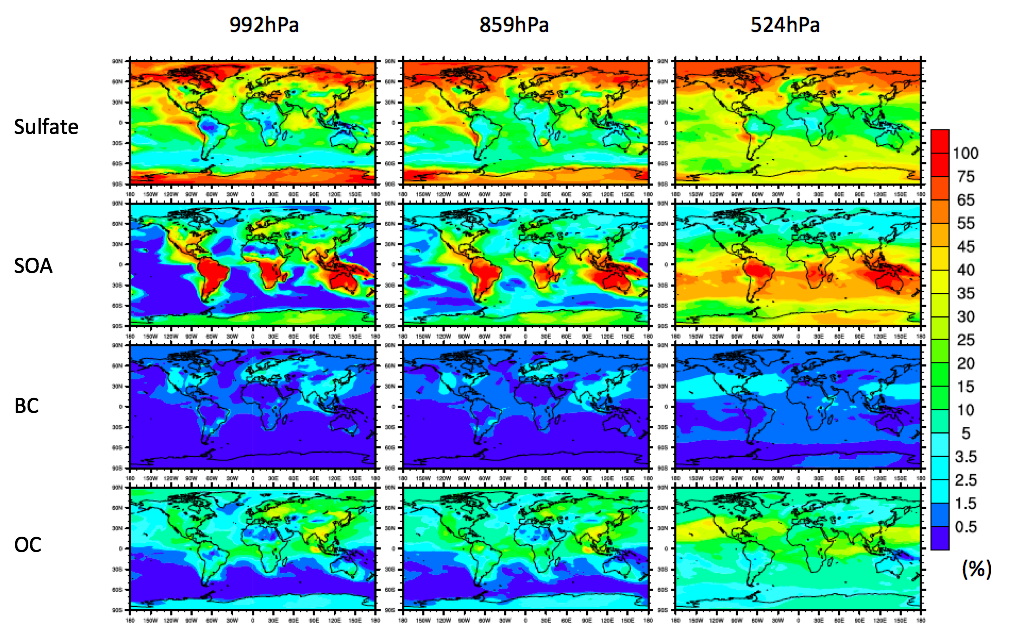
\includegraphics[width = 0.9\textwidth]{Figure29}
				\caption[Annual average of the volume fraction of sulfate, secondary organic aerosol (SOA), black carbon (BC) and organic carbon (OC) in the accumulation mode]{\label{fig_P29} Annual volume fraction of sulfate, secondary organic aerosol (SOA), black carbon (BC) and organic carbon (OC) in the accumulation mode.}
			\end{center}
		\end{figure}
			\begin{figure}[h] 
				\begin{center}
					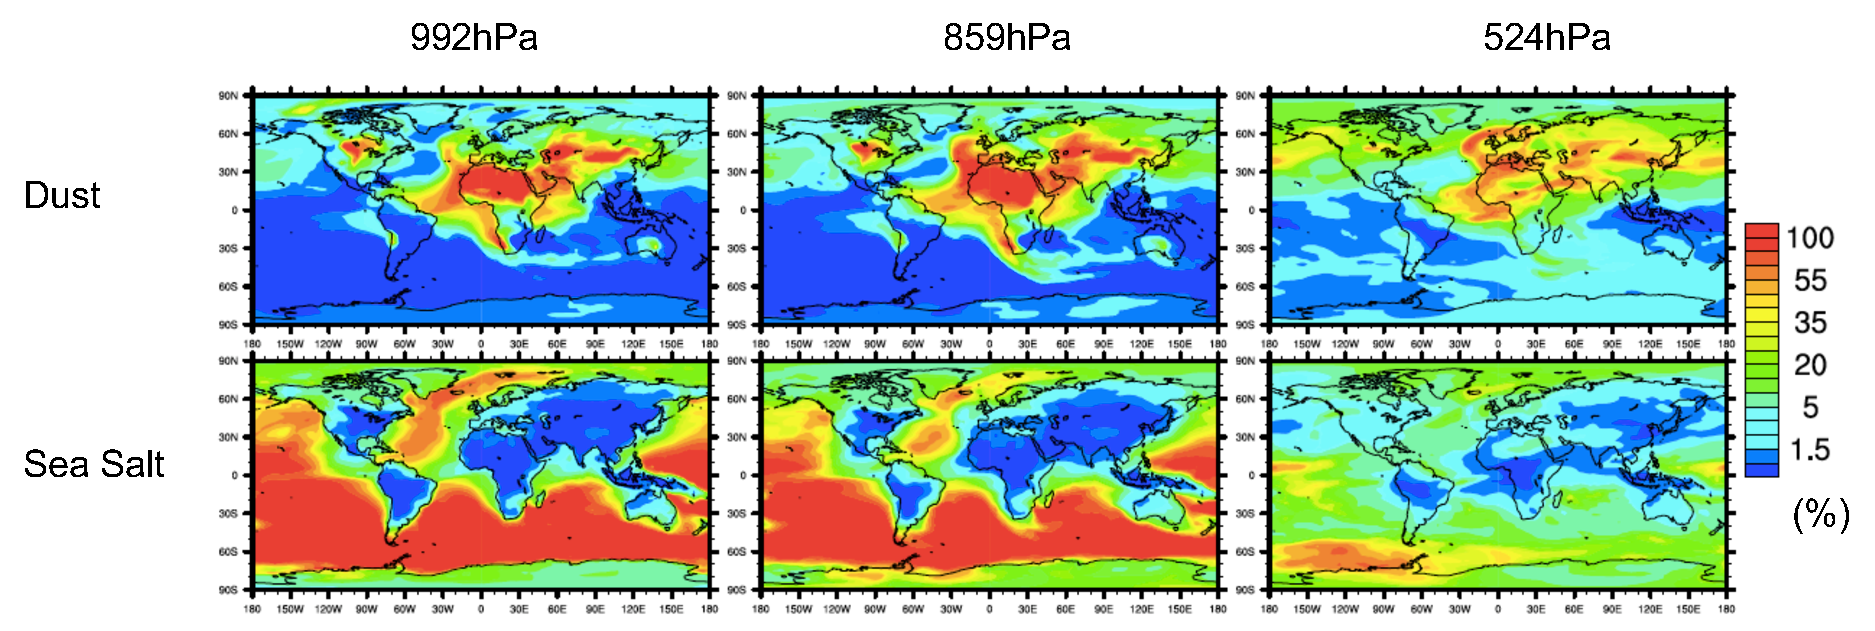
\includegraphics[width = 0.95\textwidth]{Figure30}
					\caption[Annual volume fraction of dust and sea salt (SST) near the surface (992hPa) in the accumulation mode]{\label{fig_P30} Annual volume fraction of dust and sea salt (SST) near the surface (992hPa) in the accumulation mode.}
				\end{center}
			\end{figure}
				\begin{figure}[h] 
					\begin{center}
						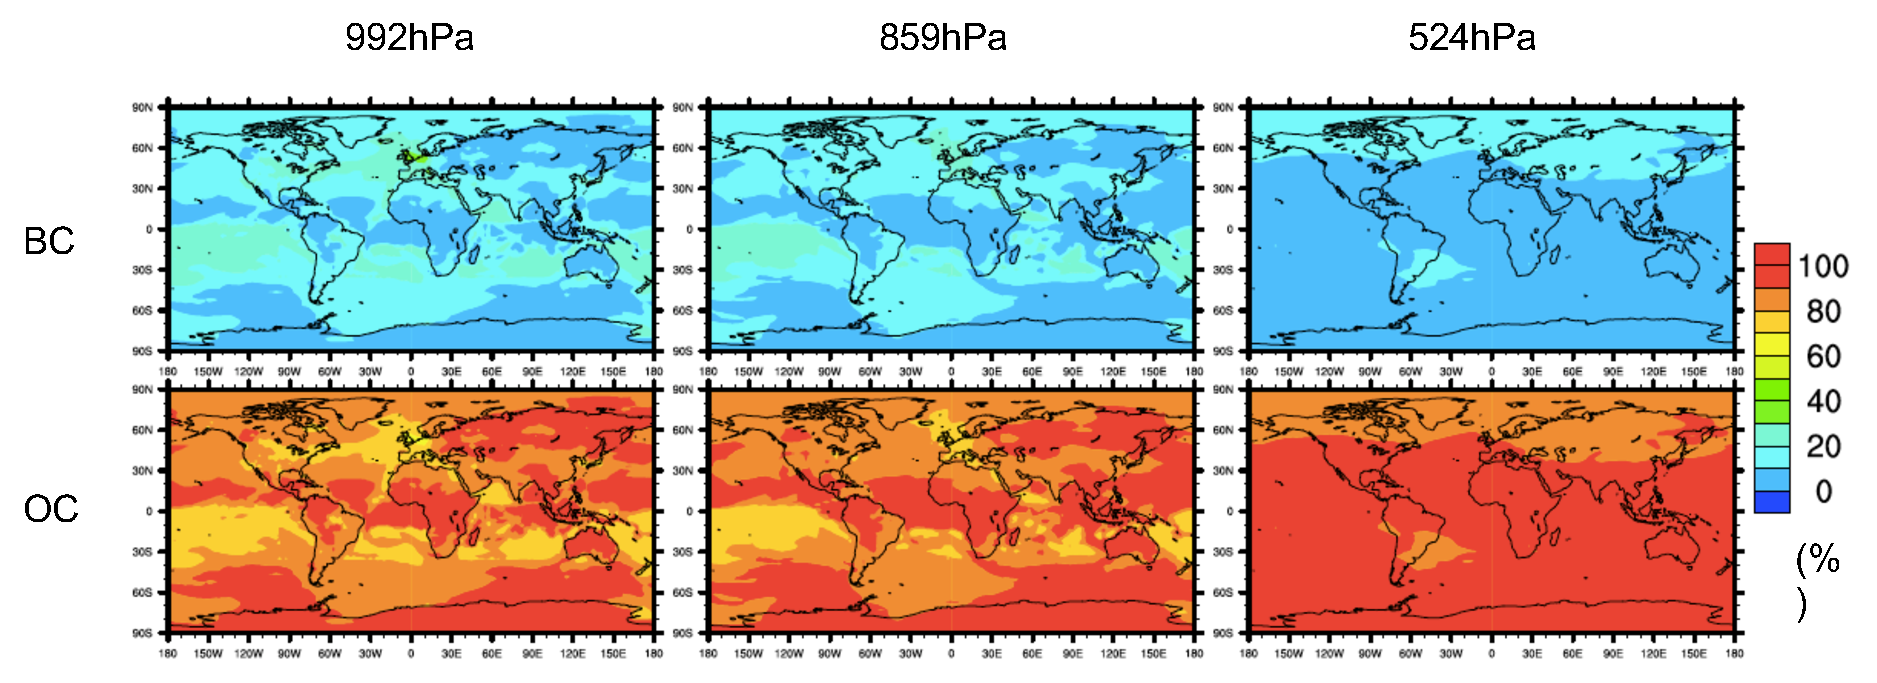
\includegraphics[width = 0.9\textwidth]{Figure31}
						\caption[Annual volume fraction of black carbon (BC) and organic carbon (OC) near the surface (992hPa) in the primary carbon mode]{\label{fig_P31} Annual volume fraction of black carbon (BC) and organic carbon (OC) near the surface (992hPa) in the primary carbon mode.}
					\end{center}
				\end{figure}
	\subsection{BC Mixing States Sensitivity to the Aging Criterion} 
	The mixing state of atmospheric BC particles with those hydrophilic aerosol components can affect both their CCN/IN activities and radiative properties. Figure~\ref{fig_P19} shows the comparison of BC mixing states between two MAM4 experiments, represented by the fraction of BC mixing ratio in the accumulation mode. We noticed that L1 case has more than 90~$\%$ of BC mass in the accumulation mode almost everywhere throughout the globe. In L8 case, however, the fraction is less than 10~$\%$ for some regions in the Arctic (Greenland, Barents sea, etc.). Most of BC is in primary carbon mode are externally mixed in the Arctic that should be of our interest, considering the fact that BC has a strong climate effect in the Arctic, and its mixing states will affect its climate forcing properties such as CCN properties and optical depth properties.  
	
	We have found that the BC mixing ratios in the L1 case are consistently lower than the L8 case throughout the globe, and the simulated BC burden is most sensitive to the choices of its aging criterion at high latitudes. This is consistent with our results that the mixing level is more sensitive to the aging criterion at high latitudes. Comparing the L8 to the L1 case, the high fraction of BC in the primary carbon mode at high latitudes seems a bit confusing because we expect BC to be more internally mixed as it is transported to distant regions. It can be understood that most BC in the Arctic comes from the nearby sources. Considering that the amount of condensible materials are relatively lower in the Arctic than in low latitudes, most of the BC remains in the primary BC mode in the L8 case. However, in the L1 case, the transfer occurs very quickly because only a small amount of condensible substances are necessary, therefore more BC gets put in the accumulation mode. The spatial sensitivity of BC mixing level to latitudes is larger in September, considering there is stronger seasonal precipitation in NH Summer (e.g., monsoon season). 
	
	In the next section, we will also discuss whether the SP2 observed BC can be representative of the total BC especially in the Arctic region. We will show that most of BC detected by SP2 measurements is also externally mixed in the Arctic, and SP2 can capture most of BC in accumulation mode (internally mixed) when it is close to the source regions.
	
	\begin{figure}[h] 
		\begin{center}
			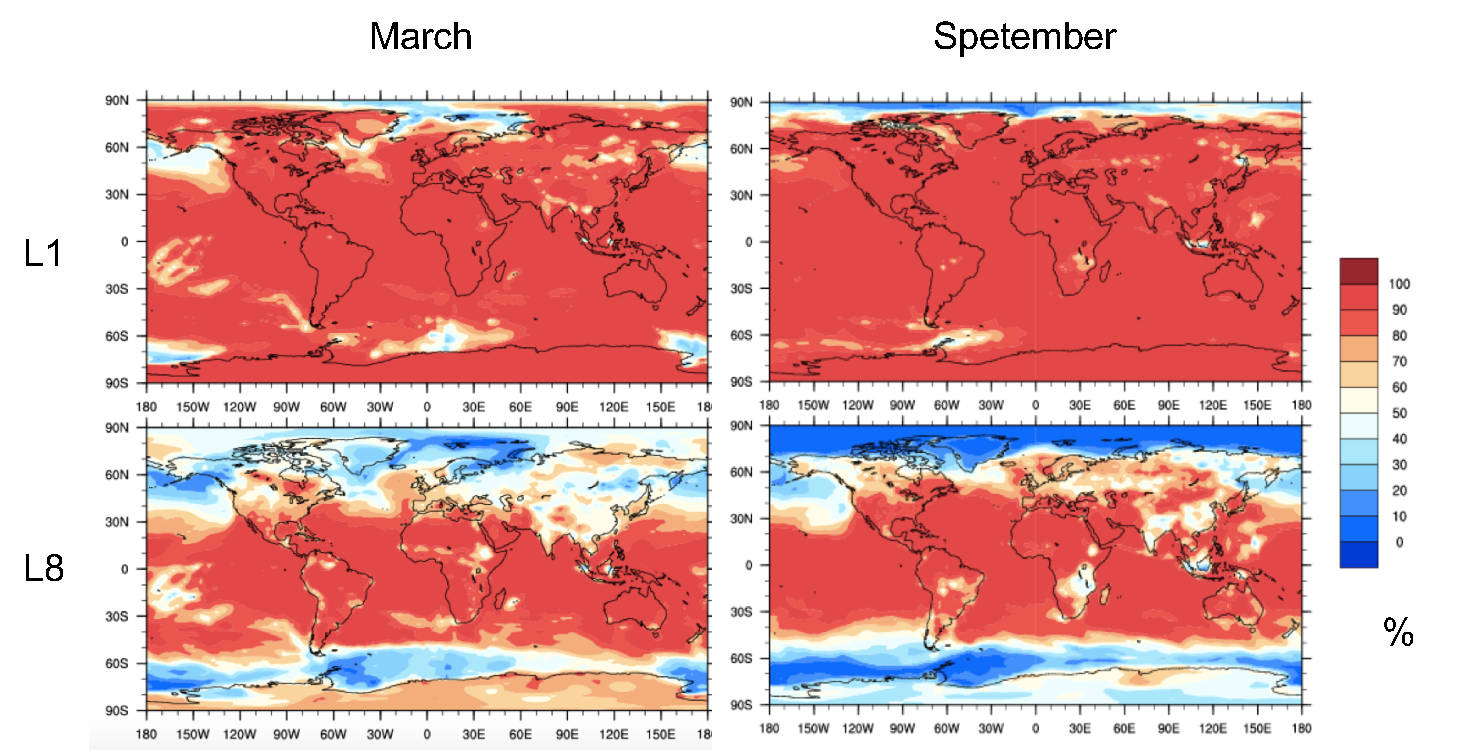
\includegraphics[width = 1\textwidth]{Figure19}
			\caption[The fractions of BC mass in the accumulation mode (in $\%$) for L1 case (top panels) and L8 case (bottom panels) in March (left panels) and September (right panels)]{\label{fig_P19}The fractions of BC mass in the accumulation mode (in $\%$) for L1 case (top panels) and L8 case (bottom panels) in March (left panels) and September (right panels).}
		\end{center}
	\end{figure}
	
	\section{Mass Fraction and Mixing States as would be Observed by SP2 measurements}
	The SP2 instrument measures the BC particle cores over a calibrated volume equivalent diameter (VED) range of 55--400~nm, which is unlikely to represent the total
	ambient number and mass concentrations of BC particles \citep{Reddington2013}. For example, \citet{Reddington2013} has found that the model predicted BC particle number concentrations a factor of 3.5–-5.7 higher than measured and more than 90~$\%$ of the model particles with dry diameters 260 nm contain BC, while the observations suggest only 14~$\%$ on average. Considering that one possible contribution to this substantial mismatch can be due to the failure of SP2 measurements to detect BC in all sizes, in this study, we estimated the mass fraction of modeled BC in the size range corresponding to SP2 measurements. SP2 number-detection efficiency at sea level pressure is reported to be 100$\%$ for BC above 90~nm VED \citep{schwarz2010global}, so following \citet{Reddington2013}, we use 90~nm--400~nm as the efficient diameter range of SP2 measurements in this study.
	
	\subsection{BC Core Diameter} 
	MAM4 assumes a lognormal distribution for each mode. Regarding the composition of each mode, the following assumptions are made: each mode contains several species (see Figure~\ref{fig_P1}), and the model tracks the species volume or mass fractions within the modes. Beyond this information, an assumption needs to be made how the species within each mode are distributed across the particle population. One usually assumes that the particle population is internally mixed within each mode, i.e. the volume fractions of the individual species do not depend on size. In other words, we assume that each particle in a mode has the same composition, and this composition is equal to the average composition of the mode. 
	In this study, before we can estimate the volume fraction of BC within the SP2 measurement size range, we first derive the geometric mean diameter of the BC core distribution. 
	
	The mean diameter of BC core can be calculated as:
	\begin{align*}
	d_{\rm g} = (d_{\text{mixed}}^3 \times f_{\text{BC}})^\frac{1}{3}, 
	\end{align*}
	where $d_{\text{mixed}}$ is the geometric mean diameter of the accumulation mode, and $f_{\text{BC}}$ is the volume
	fraction of BC in accumulation mode. For the following estimation of volume fraction within the SP2 measurement size range, we refer to the geometric mean diameter of BC particles as its core diameter.
	
	\subsection{Volume Fraction Within the Size Range of SP2 Measurement}
	The CDF of the lognormal number distribution of the BC cores in the diameter range between $d_{1}$ and
	$d_{2}$ is:
	\begin{align*}
	N(d_{1}, d_{2}) = \frac{1}{\text{ln}\sigma_{\text{g}}\sqrt{2\pi}}\int_{d_{1}}^{d_{2}}e^-\frac{(\text{ln}d - \text{ln}d_{\rm g})^2}{2\text{ln}^2\sigma_{\text{g}}}\text{d}(\text{ln}d),
	\end{align*}
	where $d_{\rm g}$ is the geometric mean diameter of the BC core distribution (extracted from the model, varying temporally and spatially). 
	
	The third moment of the lognormal distribution of BC core between 90 and 400~nm $M_{3}(d_{1}, d_{2})$ (proportional to the volume of BC cores whose diameter is within that size range) is:
	\begin{align*}
	M_{3}(d_{1}, d_{2}) &= \frac{1}{\text{ln}\sigma_{\text{g}}\sqrt{2\pi}}\int_{d_{1}}^{d_{2}}d^3e^-\frac{(\text{ln}d - \text{ln}d_{\rm g})^2}{2\text{ln}^2\sigma_{\text{g}}}\text{d}(\text{ln}d)  \\
	&=\frac{e^{\frac{k^2}{2}\text{ln}^2\sigma_{\rm g}+k\text{ln}d_{\rm g}}}{\text{ln}\sigma_{\text{g}}\sqrt{2\pi}}\int_{d_{1}}^{d_{2}}d^3e^-\frac{(\text{ln}d - \text{ln}d_{\text{gv}})^2}{2\text{ln}^2\sigma_{\text{g}}}\text{d}(\text{ln}d),
	\end{align*}
	where the geometric mean diameter of BC volume is represented as $\text{ln}d_{\text{gv}}
	= \text{ln}d_{\text{g}} + 3\text{ln}\sigma_{\text{g}}$
	
	So the mass fraction of the BC cores in the size range between $d_{1}$ and $d_{2}$ (in each mode) is derived as:
	
	\begin{align*}
	F(d_{1}, d_{2}) &= \frac{\frac{1}{\text{ln}\sigma_{\text{g}}\sqrt{2\pi}}\int_{d_{1}}^{d_{2}}d^3e^-\frac{(\text{ln}d - \text{ln}d_{\rm g})^2}{2\text{ln}^2\sigma_{\text{g}}}\text{d}(\text{ln}d)}
	{\frac{1}{\text{ln}\sigma_{\text{g}}\sqrt{2\pi}}\int_{-\infty}^{+\infty}d^3e^-\frac{(\text{ln}d - \text{ln}d_{\rm g})^2}{2\text{ln}^2\sigma_{\text{g}}}\text{d}(\text{ln}d)}  \\
	&=\frac{\frac{e^{\frac{k^2}{2}ln^2\sigma_{\rm g}+k\text{ln}d_{\rm g}}}{\text{ln}\sigma_{\text{g}}\sqrt{2\pi}}\int_{d_{1}}^{d_{2}}e^-\frac{(\text{ln}d - \text{ln}d_{\text{gv}})^2}{2\text{ln}^2\sigma_{\text{g}}}\text{d}(\text{ln}d)}{\frac{e^{\frac{k^2}{2}ln^2\sigma_{\rm g}+k\text{ln}d_{\rm g}}}{\text{ln}\sigma_{\text{g}}\sqrt{2\pi}}\int_{-\infty}^{+\infty}e^-\frac{(\text{ln}d - \text{ln}d_{\text{gv}})^2}{2\text{ln}^2\sigma_{\text{g}}}\text{d}(\text{ln}d)}\\
	&=\frac{1}{\text{ln}\sigma_{\text{g}}\sqrt{2\pi}}\int_{d_{1}}^{d_{2}}e^-\frac{(\text{ln}d - \text{ln}d_{\text{gv}})^2}{2\text{ln}^2\sigma_{\text{g}}}\text{d}(\text{ln}d) \\
	&=\frac{1}{2}[\text{erf}(\frac{\text{ln}d_{2} - \text{ln}d_{\text{gv}}}{\sqrt{2}\text{ln}\sigma_{\rm g}})-\text{erf}(\frac{\text{ln}d_{1} - \text{ln}d_{\text{gv}}}{\sqrt{2}\text{ln}\sigma_{\rm g}})],
	\end{align*}
	
	The above mass fraction for primary carbon mode ($F_{\text{pc}}(d_{1}, d_{2})$) and for accumulation mode ($F_{\text{accu}}(d_{1}, d_{2}$) do not add up to 1:
	\[F_{\text{accu}}(d_{1}, d_{2}) + F_{\text{pc}}(d_{1}, d_{2}) \neq 1.\]
	
	\textbf{Within the size range (90--400~nm)}, the ratios of the mass of BC cores in each mode to the total mass of BC cores are computed as:
	\begin{align*}
	f_{\text{accu}} = \frac{F_{\text{accu}}(d_{1}, d_{2})M_{\text{accu}}}{F_{\text{accu}}(\text{d}_{1}, d_{2})M_{\text{accu}}+F_{\text{pc}}(d_{1}, d_{2})M_{\text{pc}}},\\
	f_{\text{pc}} = \frac{F_{\text{pc}}(d_{1}, d_{2})M_{\text{pc}}}{F_{\text{accu}}(d_{1}, d_{2})M_{\text{accu}}+F_{\text{pc}}(d_{1}, d_{2})M_{\text{pc}}},
	\end{align*}
	\[f_{\text{accu}} + f_{\text{pc}} = 1,\]
	
	where $f_{\text{accu}}$ is the mass fraction of BC cores in
	accumulation mode, $f_{\text{pc}}$ is the mass fraction of BC cores in
	primary carbon mode, $M_{\text{accu}}$ and $M_{\text{pc}}$ are the mass mixing ratio of BC cores
	in accumulation mode and primary carbon mode, respectively.
	
	Sketch of $F$ and $f$ are shown in Figure~\ref{fig_R1}, Figure~\ref{fig_R2} and Figure~\ref{fig_R3}.
	
	\begin{figure}[h] 
		\begin{center}
			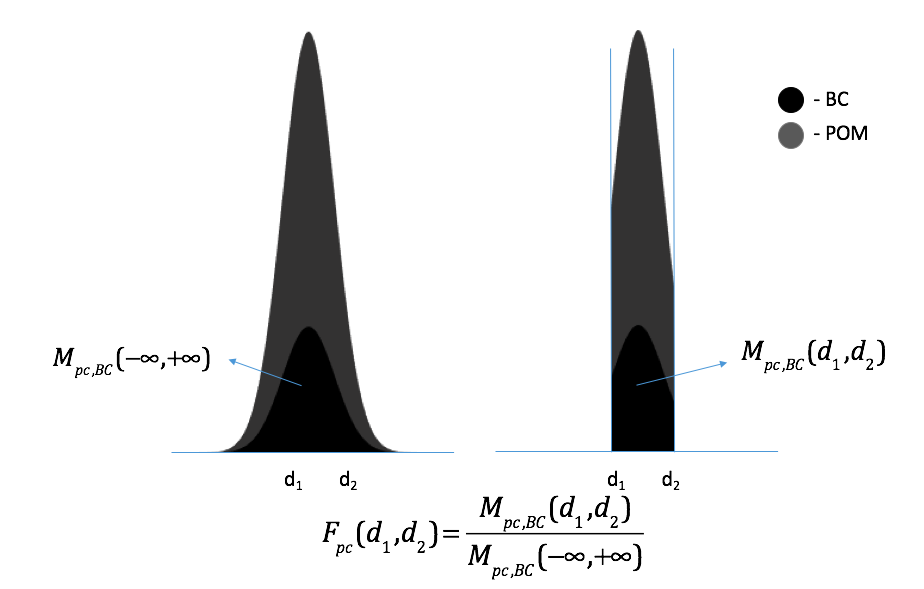
\includegraphics[width = 0.8\textwidth]{Rplot05}
			\caption[BC mass fraction within the SP2 size range for primary carbon mode $F_{\text{pc}}(d_{1}, d_{2})$]{\label{fig_R1} BC mass fraction within the SP2 size range for primary carbon mode $F_{\text{pc}}(d_{1}, d_{2})$.}
		\end{center}
	\end{figure}
	
	\begin{figure}[h] 
		\begin{center}
			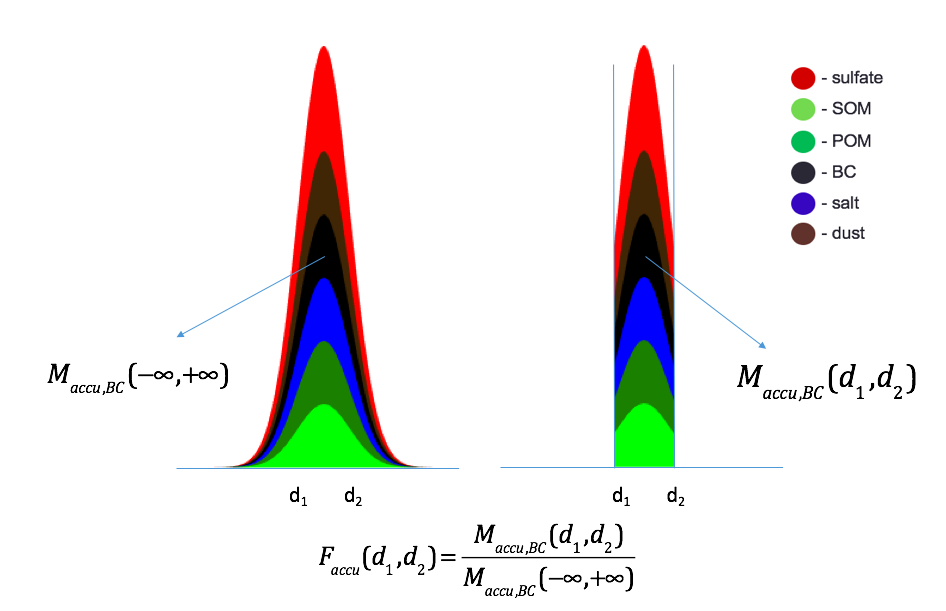
\includegraphics[width = 0.8\textwidth]{Rplot06}
			\caption[BC mass fraction within the SP2 size range for accumulation mode $F_{\text{accu}}(d_{1}, d_{2})$]{\label{fig_R2} BC mass fraction within the SP2 size range for accumulation mode $F_{\text{accu}}(d_{1}, d_{2})$.}
		\end{center}
	\end{figure}
	
	\begin{figure}[h] 
		\begin{center}
			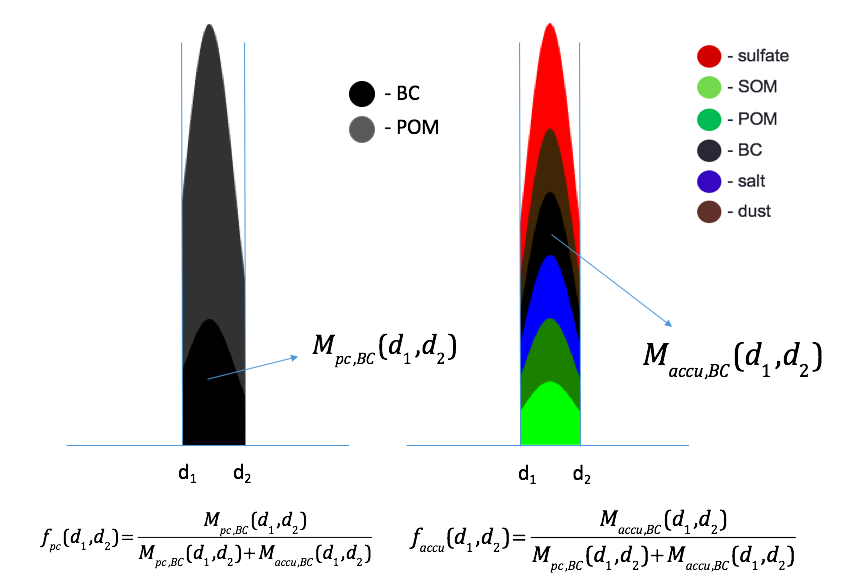
\includegraphics[width = 0.7\textwidth]{Rplot07}
			\caption[The ratios of BC mass in the SP2 size range in each mode to the total BC mass in the SP2 size range, for primary carbon mode $f_{\text{pc}}(d_{1}, d_{2})$ and for accumulation mode $f_{\text{accu}}(d_{1}, d_{2})$]{\label{fig_R3} The ratios of BC mass in the SP2 size range in each mode to the total BC mass in the SP2 size range, for primary carbon mode $f_{\text{pc}}(d_{1}, d_{2})$ and for accumulation mode $f_{\text{accu}}(d_{1}, d_{2})$.}
		\end{center}
	\end{figure}
	
	
	Generally, the mass mixing ratio of BC in the accumulation mode ($M_{\text{accu, BC}}$) is higher than that in the primary carbon mode ($M_{\text{pc, BC}}$) when it is distant from the source regions (e.g., Indian Ocean, Atlantic Ocean) (Figure~\ref{fig_R4}), primarily because black carbon will be transferred from the fresh, hydrophobic mode (primary carbon) into the aged, hydrophilic mode (accumulation) during transportation. We also observe that for some Arctic regions (e.g., Greenland), however, the BC mixing ratio can be higher in the primary carbon mode than in the accumulation mode.
	
	BC mass fractions within the SP2 size range ($F_{\text{pc}}(90~\text{nm}, 400~\text{nm})$ and
	$F_{\text{accu}}(90~\rm nm, 400~\rm nm)$) are shown in Figure~\ref{fig_R5}. For March
	(upper left panel), the SP2 measurements would be able to detect most of BC ($\textgreater$60$\%$) over the ocean and throughout the North Pole in primary carbon mode, and less of BC ($\textless$40$\%$) in regions like central Africa, Northeast Asia and Australia. This portion is higher (lower left panel) when it is close to the sources (e.g., South East Asia, Europe), and lower at high latitudes in accumulation mode. For September
	(upper right panel), however, SP2 can only detect less than $\textgreater$20$\%$ of BC in the Arctic in both modes. We also observe that the distributions of the above mass fractions (Figure~\ref{fig_R5}) have similar pattern with the size distributions of BC cores (Figure~\ref{fig_R6}), which indicates that the low values of the mass fraction ($F_{\text{pc}}(90~\text{nm}, 400~\text{nm})$ and $F_{\text{accu}}(90~\text{nm}, 400~\text{nm}$) are highly due to the small geometric mean diameter of BC cores ($\textless$90~nm)in that region. It should be noted that the unrealistically small cores come from the very small volume fraction of BC. This is an artefact of our internal-mixture assumption as is mentioned above. 
	\begin{figure}[h] 
		\begin{center}
			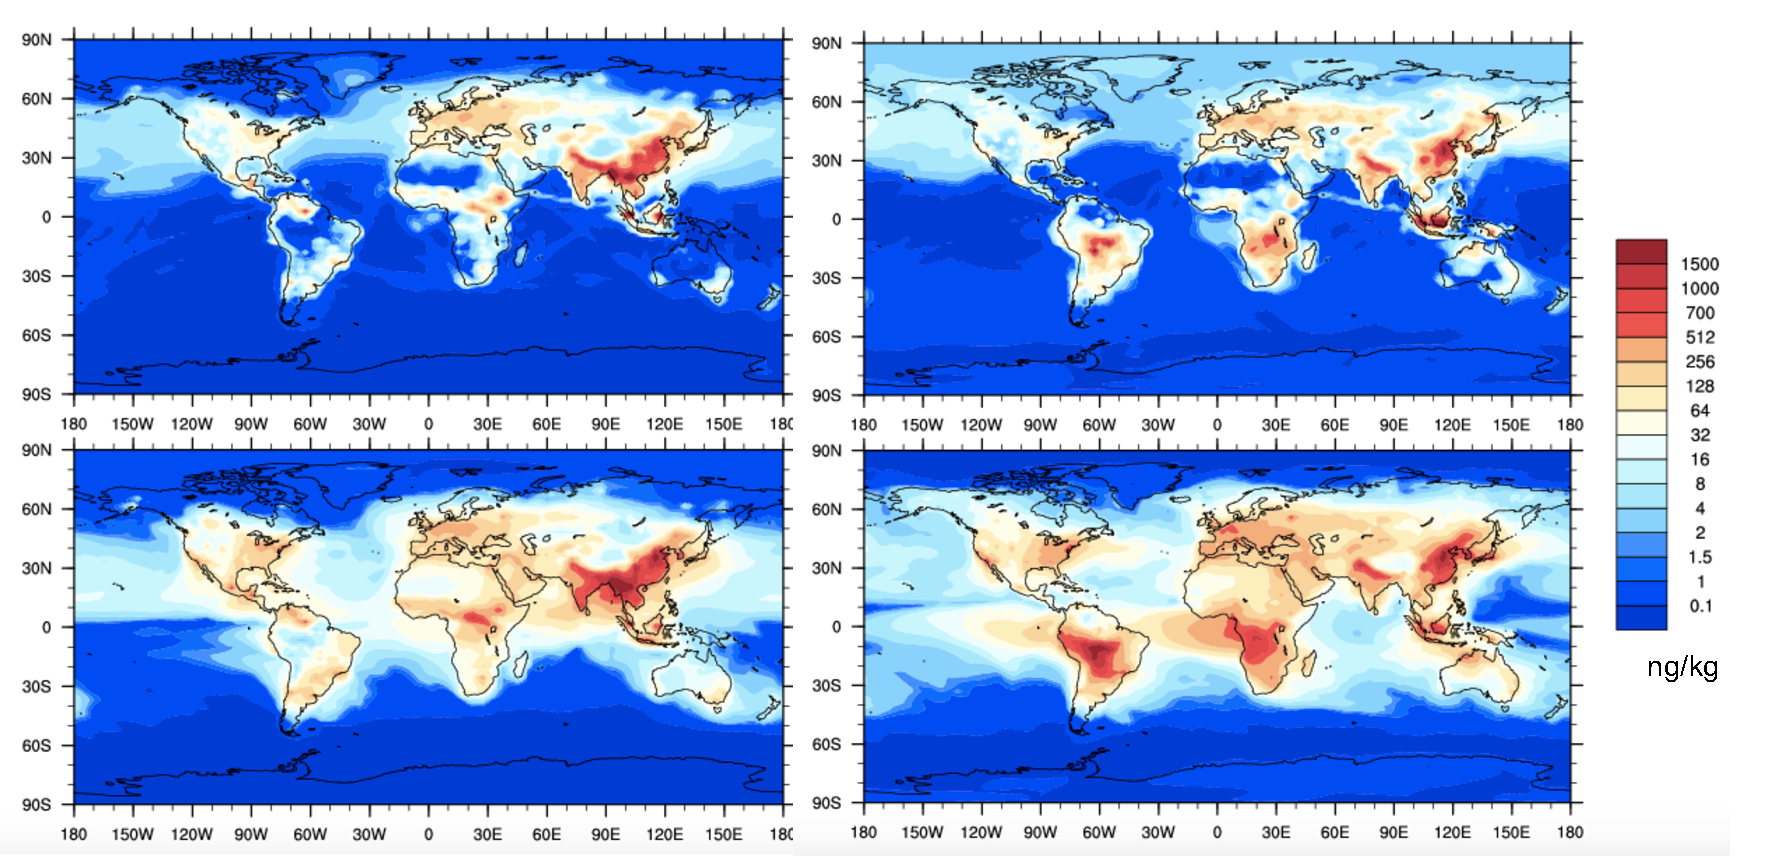
\includegraphics[width = 1\textwidth]{Rplot01}
			\caption[BC mass mixing ratio in the primary carbon mode $M_{\rm pc}$ (top) and in the accumulation mode $M_{\rm accu}$ (bottom), for surface layer, March (left) and September (right).]{\label{fig_R4}BC mass mixing ratio in the primary carbon mode $M_{\rm pc}$ (top) and in the accumulation mode $M_{\rm accu}$ (bottom), for surface layer, March (left) and September (right).}
		\end{center}
	\end{figure}
	
	\begin{figure}[h] 
		\begin{center}
			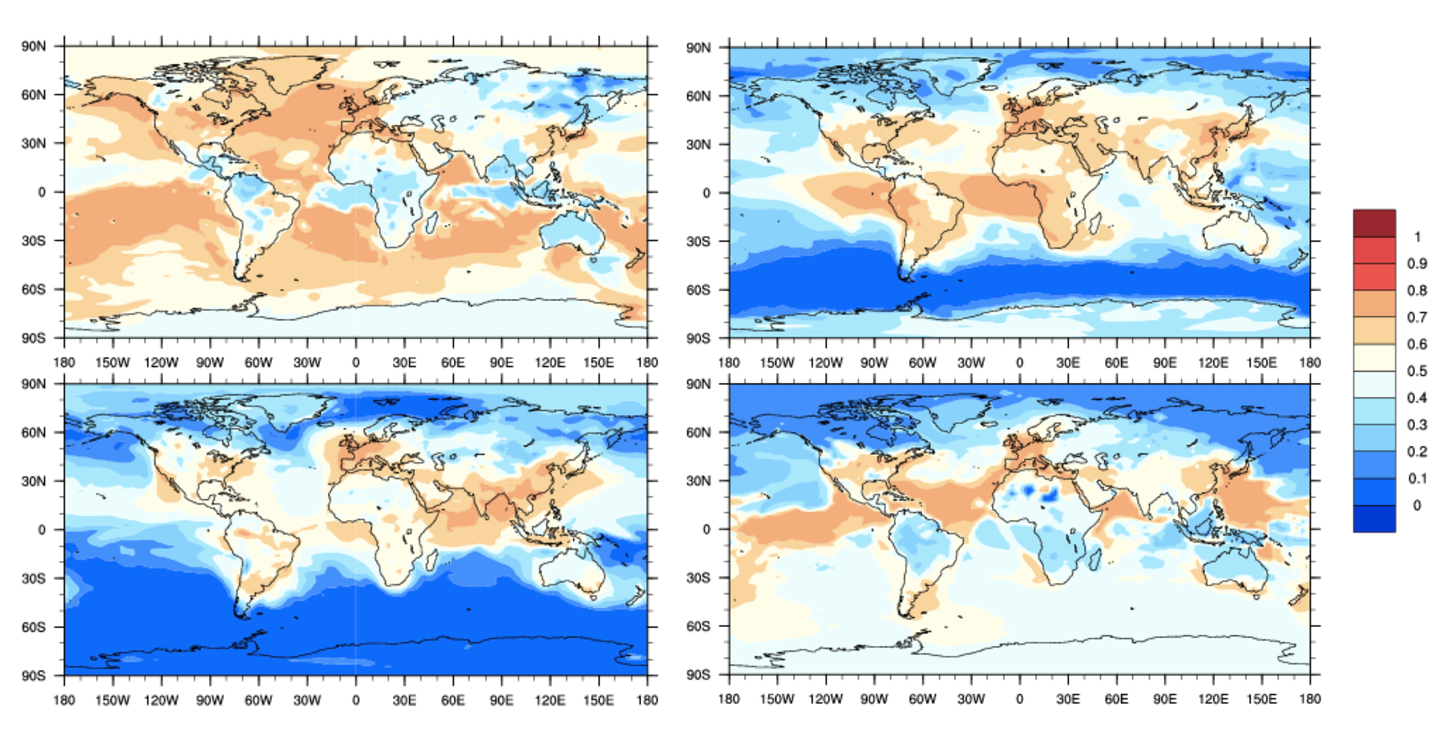
\includegraphics[width = 0.9\textwidth]{Rplot02}
			\caption[BC mass fraction between 90 and 400~nm ($F_{\rm pc}$ and $F_{\rm accu}$) in the primary carbon mode (top) and accumulation mode (bottom), for surface layer, in March and September]{\label{fig_R5} BC mass fraction between 90 and 400~nm ($F_{\rm pc}$ and $F_{\rm accu}$) in the primary carbon mode (top) and accumulation mode (bottom), for surface layer, in March (left) and September (right).}
		\end{center}
	\end{figure}
	
	\begin{figure}[h] 
		\begin{center}
			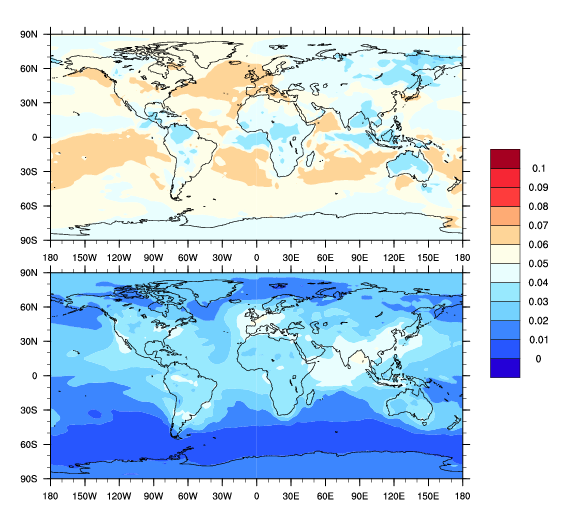
\includegraphics[width = 0.9\textwidth]{Rplot03}
			\caption[Geometric mean diameter of BC core ($\mu$m) in primary carbon mode (top) and accumulation mode (bottom), for surface layer, in March and September]{\label{fig_R6} Geometric mean diameter of BC core ($\mu$m) in primary carbon mode (top) and accumulation mode (bottom), for surface layer, in March (left) and September (right).}
		\end{center}
	\end{figure}
	
	
	
	The ratios of BC mixing ratio in each mode within the SP2 size range to the total BC mixing ratio within the SP2 size range ($f_{\rm pc}$ and $f_{\rm accu}$) are shown in Figure~\ref{fig_R7}, which represents the mixing states of BC particles that are captured by SP2 measurements. In March, most of BC aerosols are internally mixed at low and middle
	latitudes ($f_{\rm accu}\textgreater$60$\%$), whereas more of them are externally mixed at high latitudes ($f_{\rm pc}\textgreater$60$\%$). In September, the mixing state can vary spatially in the Arctic region. The above results should be taken into consideration when comparing modeled BC
	with SP2 measurements. Fractions in top and bottom panels should add up to 1.
	
	
	
	\begin{figure}[h] 
		\begin{center}
			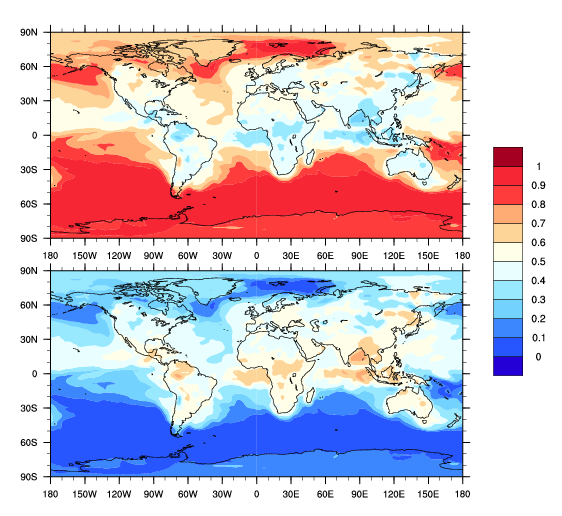
\includegraphics[width = 0.9\textwidth]{Rplot04}
			\caption[Ratio of BC mixing ratio within SP2 size range to total BC mixing ratio within SP2 size range in primary carbon mode $f_{\rm pc}$ (top) and in accumulation mode $f_{\rm accu}$ (bottom), for surface layer, in March and September]{\label{fig_R7} Ratio of BC mixing ratio within SP2 size range to total BC mixing ratio within SP2 size range in primary carbon mode $f_{\rm pc}$ (top) and in accumulation mode $f_{\rm accu}$ (bottom), for surface layer, in March (left) and September (right).}
		\end{center}
	\end{figure}
	
	

	\section{Process Analysis of BC Aging}
	\citet{Fierce2016} has derived a parameterized e-folding time $\tau_{\rm overall}$ (the derivation has been shown in Section~\ref{sec_4}) from the approximate range of condensation growth rate and number concentration for specific locations (Equation~\ref{eq_1}) 
	\begin{align}{\label{eq_1}}
	\tau_{\rm overall} \approx (k_{\rm cond}I_{\rm cond} + k_{\rm coag}N)^{-1},
	\end{align} 
	where $I_{\rm cond}$ is the condensation growth rate (in nm/h) and $N$ is the overall number concentration of aerosol particles (in $ \# \cdot \rm m^{-3}$). The condensation coefficient $k_{\rm cond} = 0.1$ and the coagulation coefficient $k_{\rm coag} = 6\times 10^{-6}$~$\text{cm}^3\text{h}^{-1}$ are determined from the regression in \citet{Fierce2016}, such that the aging timescale decreases as either $I_{\rm cond}$ or $N$ increase. The above parameterization can be used an a reference for global models. Since condensation and coagulation are independent processes, the overall aging timescale can be separated to two parts, the aging timescale due to condensation:
	\begin{align}{\label{eq_2}}
	\tau_{\rm cond} \approx (k_{\rm cond}I_{\rm cond})^{-1},
	\end{align} 
	and the aging timescale due to coagulation:
	\begin{align}{\label{eq_3}}
	\tau_{\rm coag} \approx (k_{\rm coag}N)^{-1}.
	\end{align}  
	
    In our study, we extracted $I_{\rm cond}$ and $N$ from the CAM-chem global model, and computed $\tau_{\rm overall}$, $\tau_{\rm cond}$ and $\tau_{\rm coag}$ following Equation~\ref{eq_1}, \ref{eq_2}, and \ref{eq_3}, in order to compare them to the modeled simulated aging timescales that are derived from the mass transfer rates.
	
	CAM-chem model simulated aging timescales can be derived by the following equation:
	\begin{align}{\label{eq_4}}
	\tau_{\rm CAM} = (\underbrace{\frac{\frac{\partial m_{\rm BC, cond}}{\partial t}}{m_{\rm BC, fresh}}}_{\tau_{\rm cond, CAM}^{-1}} + \underbrace{\frac{\frac{\partial m_{\rm BC, coag}}{\partial t}}{m_{\rm BC, fresh}}}_{\tau_{\rm coag, CAM}^{-1}})^{-1},
	\end{align} 
	where the mass transfer rate of BC from the primary carbon mode to the accumulation mode $\frac{\partial m_{\rm BC, cond}}{\partial t}$ (due to condensation) and $\frac{\partial m_{\rm BC, coag}}{\partial t}$ (due to coagulation) can be extracted from the model, together with the total mass of BC in the primary carbon mode $m_{\rm BC, fresh}$. The overall aging timescale $\tau$, and analogously, the aging timescale due to condensation $\tau_{\rm cond, CAM}$ and coagulation $\tau_{\rm coag, CAM}$ are then estimated according to Equation~\ref{eq_4}.
	
	\subsection{BC Condensation Growth Rate}\label{sec_3}		
	In our study, we derived the condensation growth rate $I_{\rm cond}$ as the volume condensation rate over the total aerosol surface area (in nm/h). As is mentioned in Section~\ref{sec_2}, the condensation of SOA is reversible, so the total condensation rate can be positive or negative. Since all the fresh BC particles are in the primary carbon mode, we computed the condensation growth rate using the volume condensation rate and surface area extracted from the primary carbon mode. The volume condensation rates are shown in Figure~\ref{fig_p24}. A seasonal variation can be observed where the maximum of the condensation rates occurs at 0--30~$^\circ$S during March, and at 0--30~$^\circ$N during September. Figure~\ref{fig_p24} also suggests that the distribution of $I_{\rm cond}$ are quite similar to the distributions of the SOA volume fractions in March, indicating that SOA plays a dominating role in the condensation process in spring. 
	\begin{figure}[h] 
		\begin{center}
			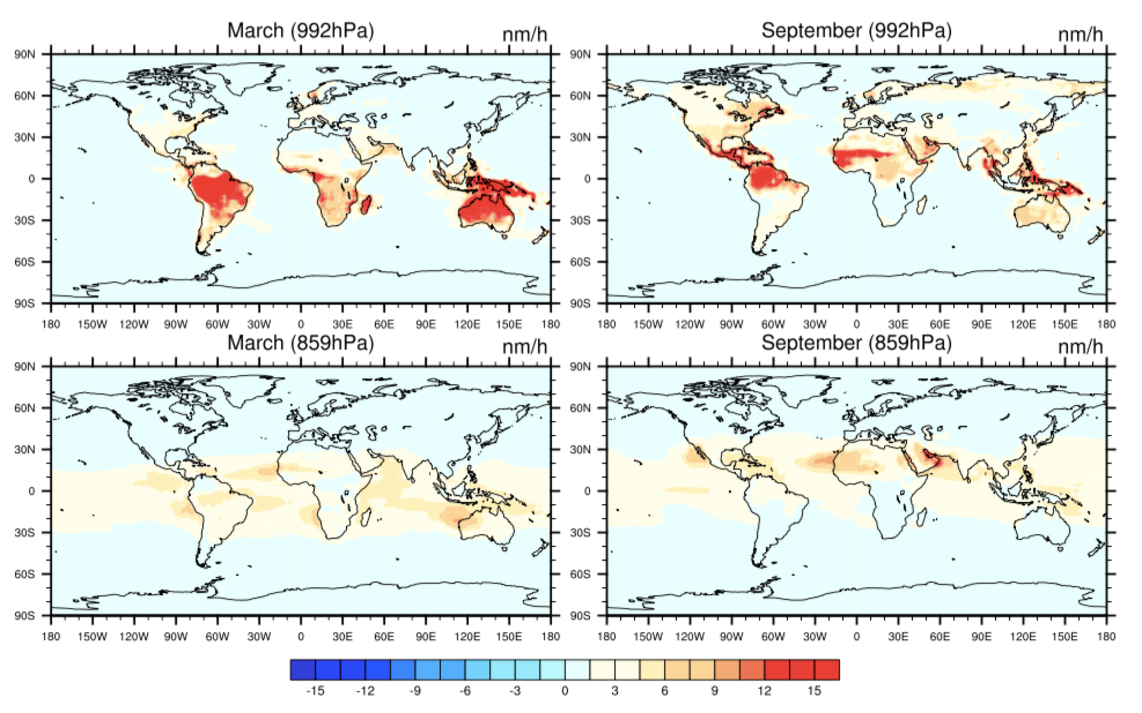
\includegraphics[width = 0.9\textwidth]{Figure24}
			\caption[Volume condensation rate ($I_{\rm cond}$) of sulfate and SOA]{\label{fig_p24} Volume condensation rate ($I_{\rm cond}$) of sulfate and SOA.}
		\end{center}
	\end{figure}
	
		
	\subsection{CAM-chem v.s. PartMC--MOSAIC Aging Timescales}
	Figure~\ref{fig_p32} and \ref{fig_p33} illustrate the CAM-chem modeled v.s. PartMC parameterization derived aging timescales near the surface and in the lower troposphere (857~hPa) respectively. We noted that the aging timescales range from less than one hour (South America) to several days (over the ocean), and these values are broadly consistent with the aging timescales from the PartMC-MOSAIC parameterization near the surface. However, the MAM4 aging timescales are slower than PartMC aging timescales in the lower troposphere as is shown in Figure~\ref{fig_p33}. We have already mentioned in Section~\ref{sec_8} that CAM is overestimating BC in upper layers. So one of the contributing factors might be the too slow aging rates. In addition, the aging rates are dominated by the relative abundance of the condensible materials and BC mass, and the condensation of SOA and sulfate plays a dominating role in BC aging.
	
	We computed the aging timescales in five sensitivity cases using an equivalent of 1, 2, 4, 6 and 8 monolayer-of-sulfate condensation criterion, represented as L1, L2, L4, L6 and L8 respectively (Figure~\ref{fig_p34}, \ref{fig_p35}). Judging from the results, when using an eight-monolayer sulfate criterion, the aging timescales near the surface have the closest linear-regression slope to 1 and the highest R$^2$ value among the five sensitivity cases. At an upper layer (857hPa), however, L6 case have the closest linear-regression slope to 1 and the highest $R^2$ value, indicating that the CAM-chem aging rates is slow biased. 

	
	\begin{figure}[h] 
		\begin{center}
			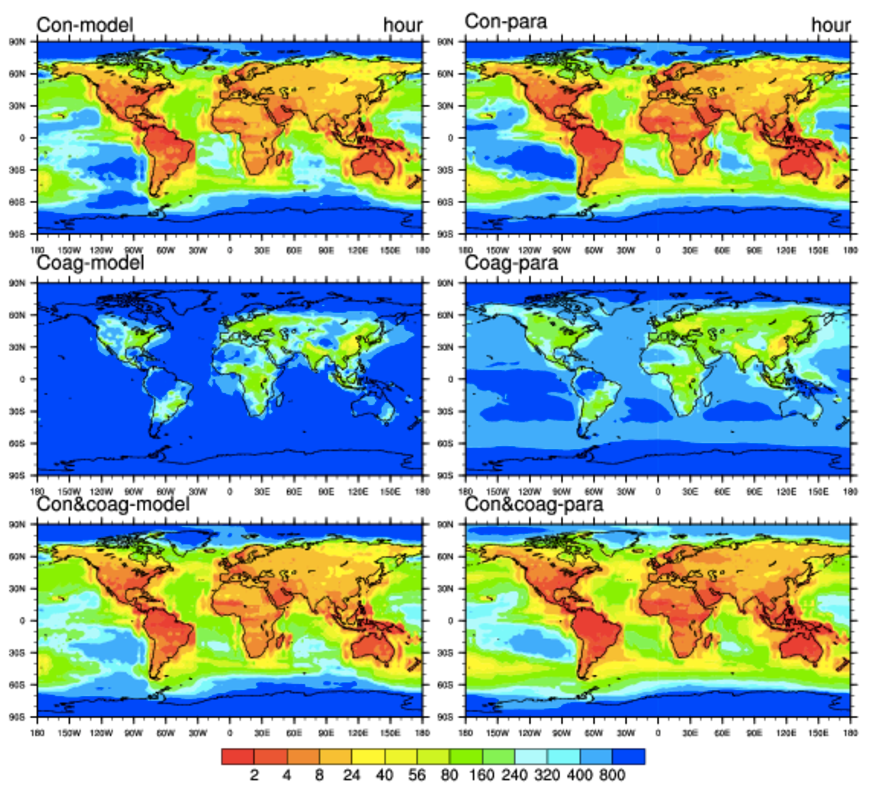
\includegraphics[width = 0.9\textwidth]{Figure32}
			\caption[Annual BC aging timescales (in hours) near the surface, extracted from the CAM-chem model (left) and computed based on PartMC-MOSAIC parameterization (right). The condensation, coagulation and overall timescales are displayed in the upper panels, middle panels and bottom panels respectively]{\label{fig_p32} Annual BC aging timescales (in hours) near the surface, extracted from the CAM-chem model (left) and computed based on PartMC-MOSAIC parameterization (right). The condensation, coagulation and overall timescales are displayed in the upper panels, middle panels and bottom panels respectively.}
		\end{center}
	\end{figure}

	\begin{figure}[h] 
		\begin{center}
			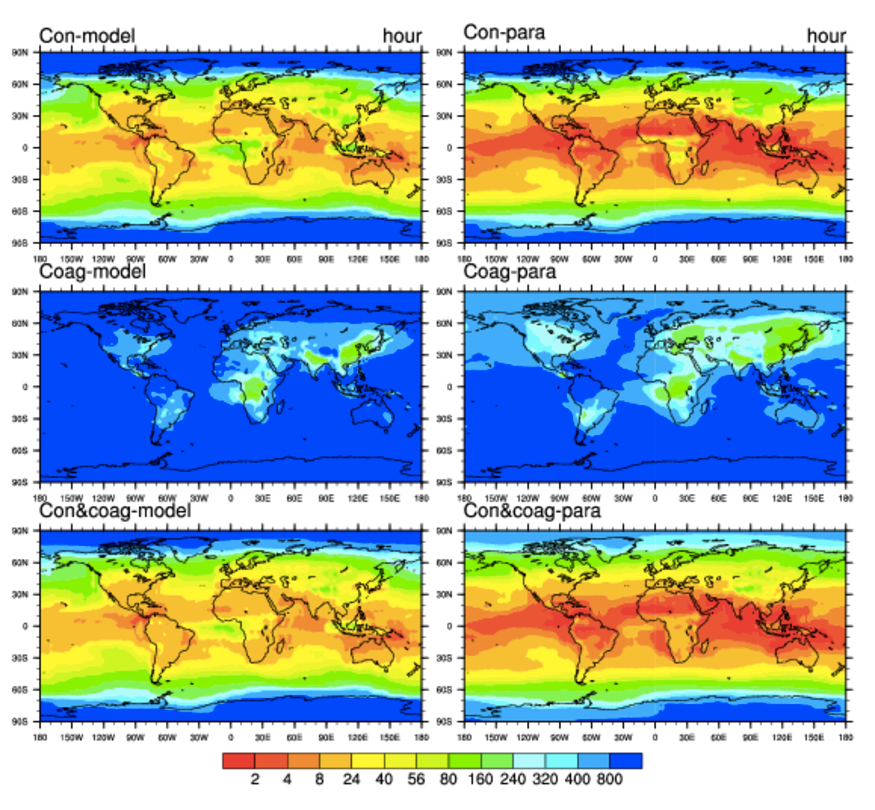
\includegraphics[width = 0.9\textwidth]{Figure33}
			\caption[Annual BC aging timescales (in hours) at 857~hPa, extracted from the CAM-chem model (left) and computed based on PartMC-MOSAIC parameterization (right). The condensation, coagulation and overall timescales are displayed in the upper panels, middle panels and bottom panels respectively]{\label{fig_p33} Annual BC aging timescales (in hours) at 857~hPa, extracted from the CAM-chem model (left) and computed based on PartMC-MOSAIC parameterization (right). The condensation, coagulation and overall timescales are displayed in the upper panels, middle panels and bottom panels respectively. }
		\end{center}
	\end{figure}
	
	\begin{figure}[h] 
		\begin{center}
			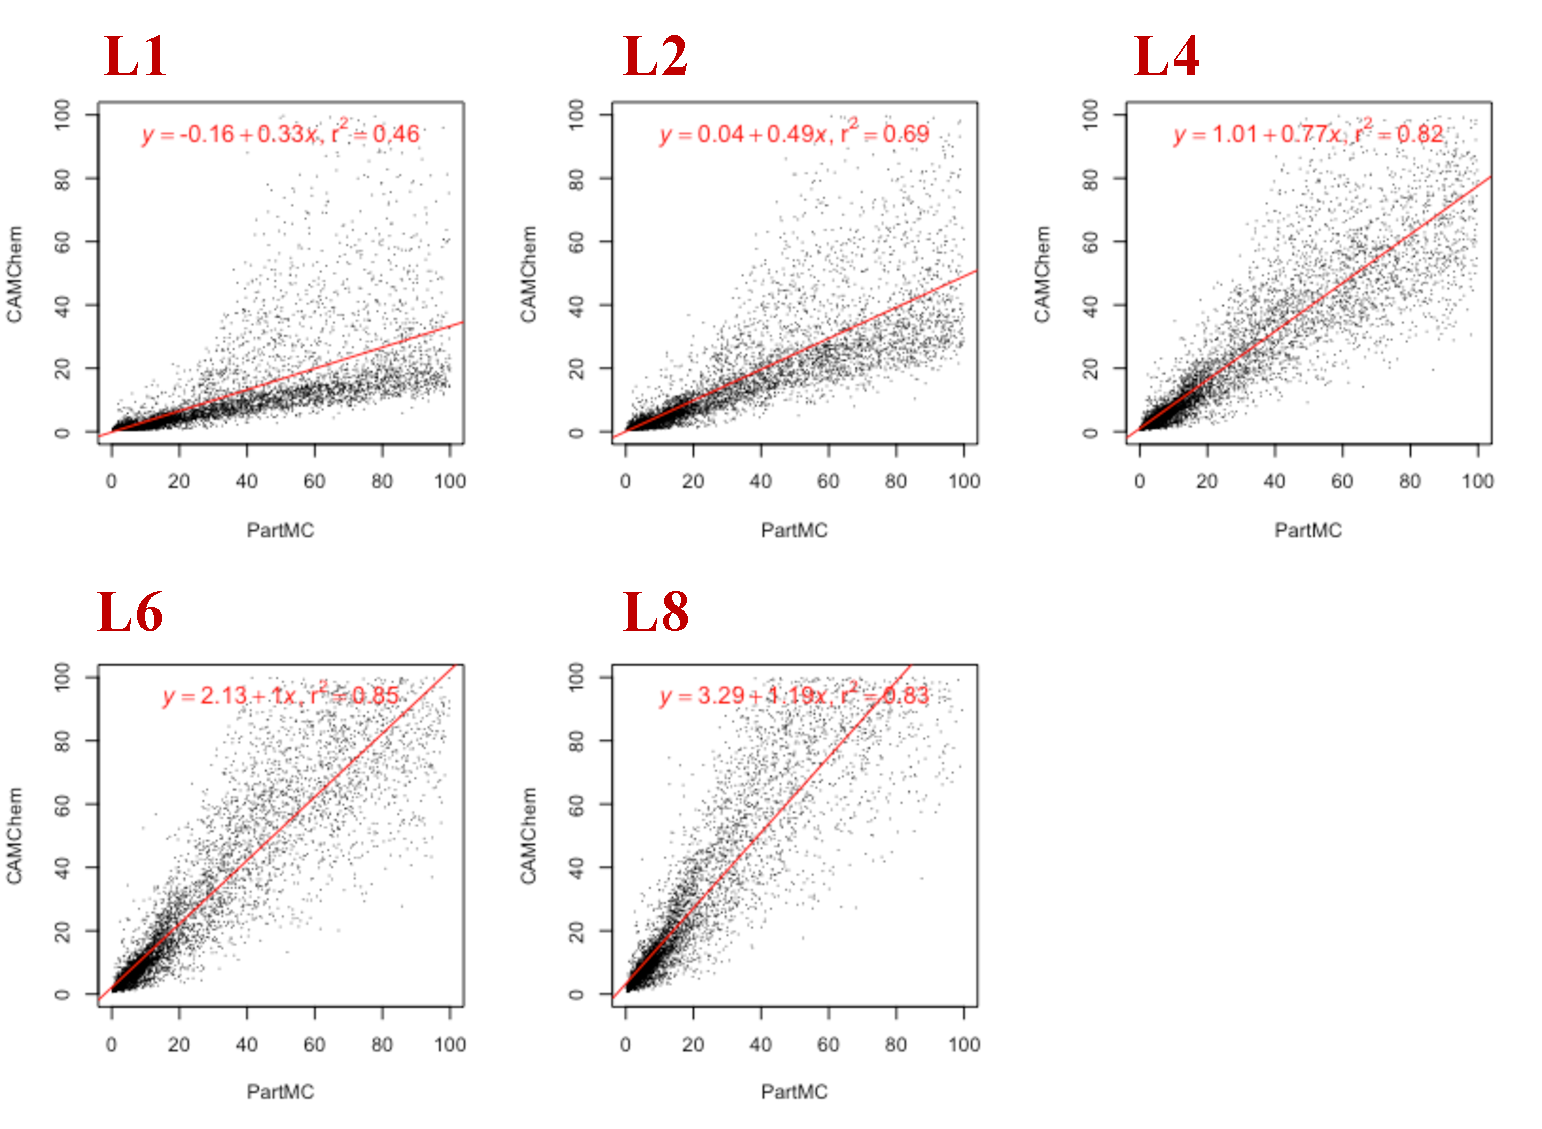
\includegraphics[width = 0.9\textwidth]{Figure34}
			\caption[Scatter plots of CAM-chem v.s. PartMC--MOSAIC aging timescales (in hour) near the surface in 5 sensitivity cases. L1--L8 represents the number of monolayers (1 to 8) for the condensation criterion]{\label{fig_p34} Scatter plots of CAM-chem v.s. PartMC--MOSAIC aging timescales (in hour) near the surface in 5 sensitivity cases. L1--L8 represents the number of monolayers (1 to 8) for the condensation criterion.}
		\end{center}
	\end{figure}
	
	
	\begin{figure}[h] 
		\begin{center}
			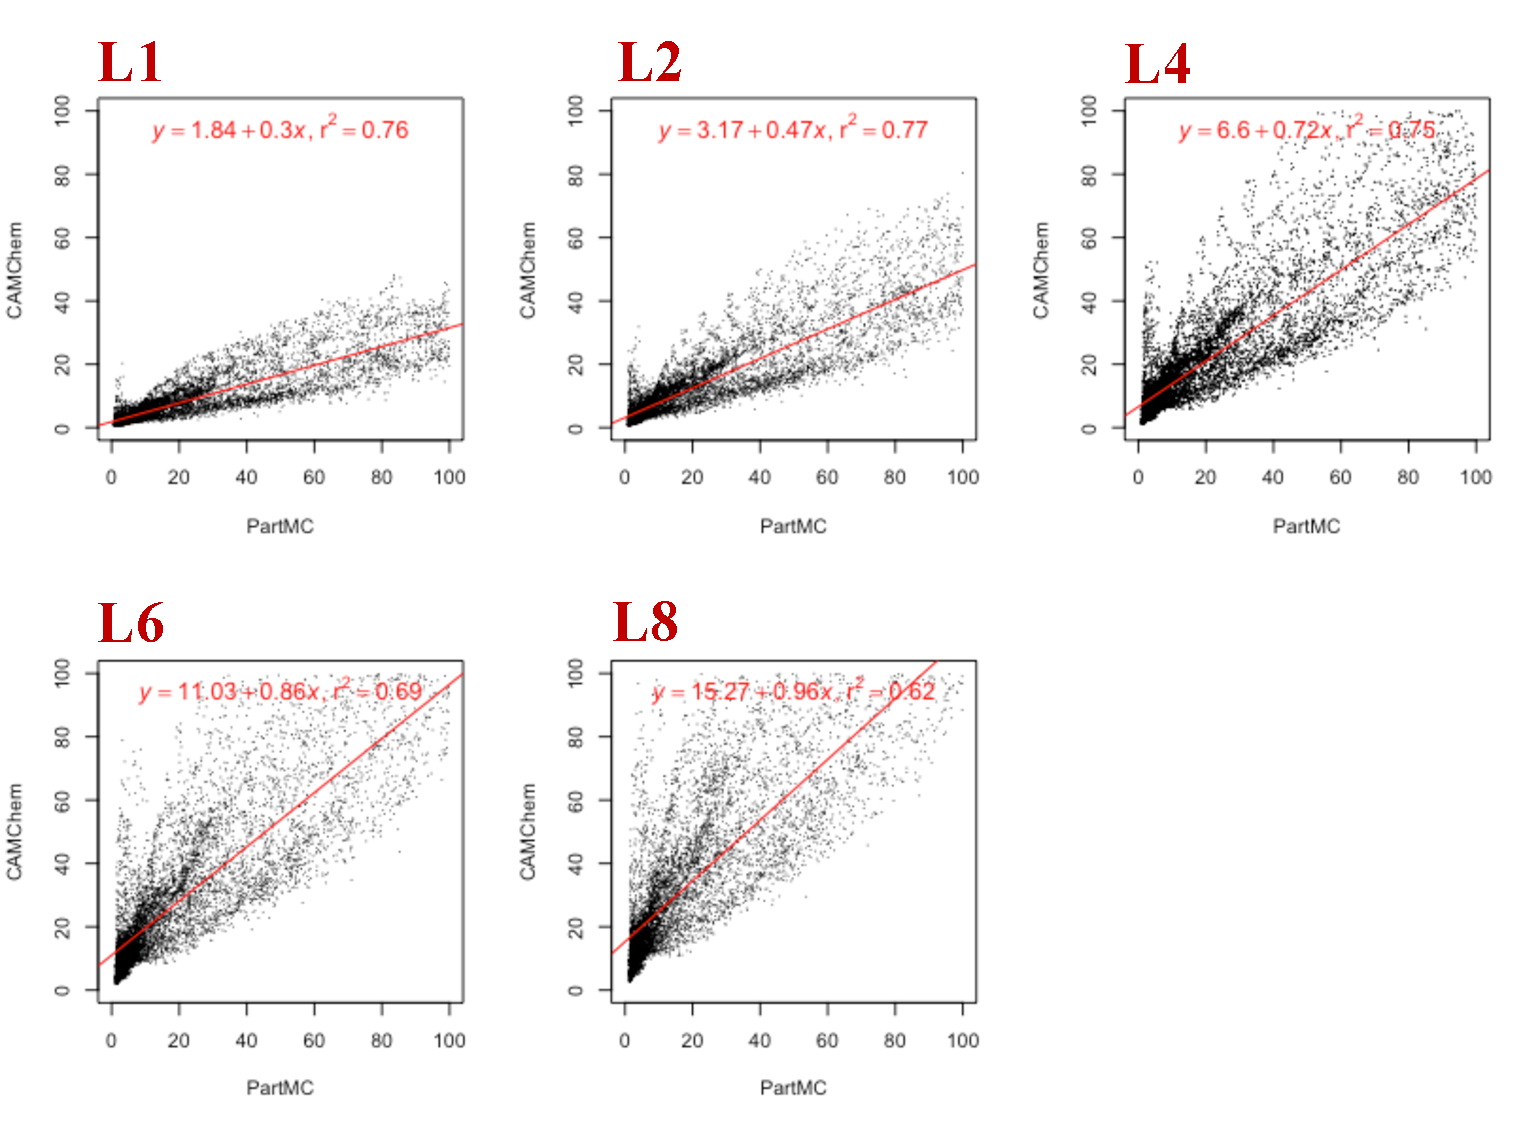
\includegraphics[width = 0.9\textwidth]{Figure35}
			\caption[Scatter plots of CAM-chem v.s. PartMC--MOSAIC aging timescales (in hour) at 857~hPa in 5 sensitivity cases. L1--L8 represents the number of monolayers (1 to 8) for the condensation criterion]{\label{fig_p35} Scatter plots of CAM-chem v.s. PartMC--MOSAIC aging timescales (in hour) at 857~hPa in 5 sensitivity cases. L1--L8 represents the number of monolayers (1 to 8) for the condensation criterion.}
		\end{center}
	\end{figure}
	
	
	\chapter{Summary and Conclusion}
		In this study, the representation of BC aerosols in CAM--chem MAM4 model has been assessed. Several sensitivity runs were conducted to investigate the extent to which BC burden, mixing states and radiative forcing is sensitive to the choices of aging parameters. Furthermore, a new method was applied to evaluate the accuracy of BC aging represented in CAM--chem model, by comparing BC aging rates extracted from CAM-chem to aging parameterization based on more detailed particle-resolved simulations with PartMC-MOSAIC. The parameterization was obtained from \citet{Fierce2016}. 
		
		We used four-mode version of the modal aerosol model (MAM4) in CAM--chem, where the aging process was represented by the conversion of BC aerosol particles from the hydrophobic, primary carbon mode to the hydrophilic, accumulation mode after coating with certain amount of species by condensation, and by coagulation. In order to explore the model sensitivity to the aging criterion, we conducted four simulations from January 1, 2010, to December 31, 2010, by setting the threshold of monolayers to 1, 2, 4 and 8 to determine the mass transfer rate between the two modes. Generally, increasing the number of mono-layers implies that larger amount of sulfate or SOA will be needed to age the primary carbonaceous particles into the accumulation mode. Consequently, particles will stay for longer in the primary carbon (no wet deposition) mode before moving into the accumulation mode (subject to wet deposition), hence BC can transport longer distances, and its residence time in the atmosphere is longer. 
		
		We also explored the sensitivity of BC deposition flux and burden to the aging criterion, and computed the relative differences between two cases (L1 v.s. L8). Both wet and dry scavenging rates are most sensitive to the choices of aging criterion at high latitudes, with the maximum relative differences around 90~$\%$ in the Arctic. A seasonal cycle can be observed. Similarly, we found that BC burden is also most sensitive to the aging criterion at high latitudes where the background concentrations are low, with maximum differences in the annually averaged BC mixing ratio of 16$\%$ near the surface. For the Arctic region, the maximum relative differences of 71~$\%$ can be at high altitudes around 400 hPa. We also analyzed the sensitivity of BC radiative forcing to the aging criterion. The magnitude of annually and spatially averaged radiative forcing is 0.18~W$\cdot{\text{m}^{-2}}$ in the L1 case, lower than that of 0.48~W$\cdot{\text{m}^{-2}}$ in the L8 case because the BC burden is smaller for the L1 case with faster aging and wet deposition. Regionally, the magnitudes of BC radiative forcing are higher with a maximum of around 15~W$\cdot{\text{m}^{-2}}$ in Northeastern China. 

		The mixing state of BC particles with those hydrophilic aerosol components can affect both their CCN/IN activities and radiative properties and should be of our interest. So we computed BC mass fraction and their mixing states, and focused our study in the Arctic region where the climate is more sensitive to BC concentrations. We found that more than 90~$\%$ of BC mass is simulated to be in primary carbon mode (externally mixed) and only less than 10~$\%$ of them are in the accumulation mode (internally mixed). We also noticed that the simulated BC distribution is often outside the range of what an SP2 instrument can detect. Our results indicated that in the Arctic, more than 60~$\%$ of BC mass can be detected in March, whereas only less than 20~$\%$ of BC mass can be detected in September. This result, albeit preliminary, should be taken into consideration when comparing model simulated BC with SP2 observed data in the Arctic. 
 
		Our above results have shown that BC related properties are very sensitive to the choices of aging parameters in the climate model. So it is important to evaluate whether a model representation of BC aging is 'correct'. Currently, no observed data of aging rates is available, and more generally, it is hard to compare a ‘process’ to observed data. In CAM-chem, the treatment of BC aging is based on simplified assumptions, computing mechanic transfer rates by assuming aerosol size distributions, mixing levels and number-of-monolayer criterion. However, PartMC-MOSAIC model tracks the evolution of individual particles (mass constituent aerosol species), where the processes of advection, diffusion and coagulation are modeled stochastically. It has the advantage that no specific aging criterion assumption is required. So in our study, we implemented a new method by exploiting PartMC-MOSAIC parameterizations based on more detailed particle resolved simulations as reference to evaluate the performance of MAM4 aging scheme. We found that CAM-chem annual aging timescales range from less than one hour to several days, where condensation plays a dominating role. The comparison indicates that PartMC--MOSAIC timescales are broadly consistant with CAM-chem timescales near the surface, whereas they are lower than CAM-chem aging timescales in an upper layer (857~hPa), indicating faster aging rates. These results can be used as reference for further CAM-chem model development.
		
		We have already analyzed the model sensitivity to the number of monolayers. The aging criterion assumed that the particle sizes in each mode follow a lognormal distribution where the mean diameter can evolve with time whereas the standard deviation remains the same. Considering that the evolution of their size distribution can be affected by the model assumed BC emission diameter (134~nm by default), future work can include model sensitivity analysis to the BC emission mean diameters. Furthermore, this thesis work only focused on model simulations. So the findings can be applied to further comparison between simulated BC burden and mixing states with SP2 data (e.g., HIPPO, FAAM BAe-146, Pallas Global Atmosphere Watch (GAW) ). However, we also noted that in our estimation of modeled BC mass fraction corresponding to the size ranges of SP2 measurements, unrealistically small cores diameters can be derived in some regions. This is because that the model assumes all particles in the accumulation mode to be internally mixed with the same compositions, where small BC mass fraction can lead to the above problem. So for better comparison with SP2 measurements, a method to estimate the mass fraction of model simulated BC in that size range should be further developed in the future.
		
		 
		


	
	
	\chapter{Appendix}
	
	\section{Configuration of CAM-chem Model}
	Create a directory for the code, download the code, go into the scripts directory in the source code:
	\begin{lstlisting}[xleftmargin=0.01\textwidth, xrightmargin=0.01\textwidth]
	mkdir ~/cesm1_2_2_CAMChem
	cd /glade/u/home/yinruili/cesm1_2_2_CAMChem/script
	\end{lstlisting}
	
	Create a new case:
	\begin{lstlisting}[xleftmargin=0.01\textwidth, xrightmargin=0.01\textwidth]
	setenv CCSMTAG	cesm1_2_2_CAMChem
	setenv CASE	FSTRATMAM4_extract_offmeteo_5
	setenv MACH      yellowstone
	setenv CCSMROOT  /glade/u/home/yinruili/${CCSMTAG}
	setenv CASEROOT  /glade/scratch/yinruili/cases/$CASE
	# create a new case using MAM4 and free-running
	./create_newcase -case $CASEROOT -mach $MACH -res  f19_f19 -compset FSTRATMAM4
	# create a new case using MAM4 with offline-meteorology
	./create_newcase -case $CASEROOT -mach $MACH -res  f19_f19 -user_compset GEOS_CAM5%SMA4_CLM40%SP_CICE%PRES_DOCN%DOM_RTM_SGLC_SWAV 
	\end{lstlisting}
	
	Edit runtime options using xmlchange: env$\_$run.xml
	\begin{lstlisting}[xleftmargin=0.01\textwidth, xrightmargin=0.01\textwidth]
	#e.g., start at 2010-01-01, run for 12 months.
	./xmlchange  -file env_run.xml -id  STOP_N        -val '12'
	./xmlchange  -file env_run.xml -id  STOP_OPTION   -val 'nmonth'
	./xmlchange  -file env_run.xml -id  RUN_STARTDATE -val '2010-01-01'
	\end{lstlisting}
	Edit namelist: user\_nl\_cam (This file will be created after you set up the case (./cesm\_setup), but it can also be created manually (using cat) before that. I would prefer the latter option).
	\begin{lstlisting}[xleftmargin=0.01\textwidth, xrightmargin=0.01\textwidth]
	#add variables that you would like to see in the output
	cat <<EOF >! user_nl_cam
	history_aerosol     = .true.
	history_amwg        = .true.
	history_aero_optics = .true.
	mfilt           = 1,  1,
	# nhtfrq = 0, the file will be monthly average
	# nhtfrq = -24, the frequency is input as 24 hours (daily)
	nhtfrq          = 0,  -24,
	# avgflag_pertape = 'A', averaged data
	# avgflag_pertape = 'I', instantaneous data
	avgflag_pertape ='A','A',
	# variables you would like to add into monthly file (fincl1) and hourly file (fincl2)
	fincl1          ="bcgascon","bcagingcon","bcmasscon","surface","volumn","bcagingcoag","bcmasscoag","numa1","numa2","numa3","numa4", "dgnd_a01", "dgnd_a02", "dgnd_a03", "dgnd_a04", "dgnw_a01", "dgnw_a02","dgnw_a03","dgnw_a04","dgnumwet1","dgnumwet2","dgnumwet3","dgnumwet4"
	fincl2          ="bcgascon","bcagingcon","bcmasscon","surface","volumn","bcagingcoag","bcmasscoag","numa1","numa2","numa3","numa4", "dgnd_a01", "dgnd_a02", "dgnd_a03", "dgnd_a04", "dgnw_a01", "dgnw_a02","dgnw_a03","dgnw_a04","dgnumwet1","dgnumwet2","dgnumwet3","dgnumwet4"
	\end{lstlisting}
	
	Set offline meteorology:
	\begin{lstlisting}[xleftmargin=0.01\textwidth, xrightmargin=0.01\textwidth]
	inithist = 'MONTHLY'
	ncdata        = '/glade/p/cesm/cseg//inputdata/atm/cam/inic/fv/camchem_ic_2008-01-01_1.9x2.5_L56_c110118.nc'
	bnd_topo  = '/glade/p/cesm/cseg/inputdata/atm/cam/met/USGS-gtopo30_1.9x2.5_phys_geos5_c100929.nc'
	met_data_file   = '2010/GEOS5.2_19x2_20100101.nc'
	met_data_path   = '/glade/p/cesmdata/cseg/inputdata/atm/cam/met/GEOS5'
	met_filenames_list      = '/glade/p/cesmdata/cseg/inputdata/atm/cam/met/GEOS5/GEOS5_filenames_list_c120516.txt'
	met_max_rlx     = 0.10
	met_qflx_factor = 0.84
	\end{lstlisting}
	
	Configure the model:
	\begin{lstlisting}[xleftmargin=0.01\textwidth, xrightmargin=0.01\textwidth]
	./cesm_setup
	\end{lstlisting}
	
	Modify the source code and add them into ./SourceMode
	\begin{lstlisting}[xleftmargin=0.01\textwidth, xrightmargin=0.01\textwidth]
	# For example, I modified two files (al_aero_gasaerexch_sens_icon.F90 and modal_aero_coag.F90), and copied them into the SourceMode directory so that the model can be build with the modified code. 
	cp /glade/u/home/yinruili/cesm1_2_2_CAMChem/scripts/sourcemode/modal_aero_gasaerexch.F90 ./SourceMods/src.cam/modal_aero_gasaerexch.F90
	cp /glade/u/home/yinruili/cesm1_2_2_CAMChem/scripts/sourcemode/modal_aero_coag.F90 ./SourceMods/src.cam/
	
	\end{lstlisting}
	
	Build the model, and then go into the case root and run the model:
	\begin{lstlisting}[xleftmargin=0.01\textwidth, xrightmargin=0.01\textwidth]
	./$CASE.build
	cd $CASEROOT
	./$CASE.run
	\end{lstlisting}


\appendix*

\include{Appendix.tex}

\backmatter

\bibliographystyle{apalike}
\bibliography{thesis}

\end{document}
\endinput
%%
%% End of file `thesis-ex.tex'.
